\documentclass{thesis}

\usepackage{doublespace}
\usepackage{url}
\usepackage{epsfig}
\usepackage{subfigure}
\usepackage{hhline}
\usepackage{fancyhdr}
\usepackage{lettrine}
\usepackage{listings}
\usepackage{titlesec}
\usepackage{multirow}
\usepackage{longtable}
\usepackage{algorithm}
\usepackage{algpseudocode}
\usepackage[shortlabels]{enumitem}
\usepackage{nccmath}
%\usepackage[LGRx,T1]{fontenc}
\usepackage[utf8]{inputenx}
\usepackage[toc,page]{appendix}
\usepackage[greek,english]{babel}
%\usepackage[iso-8859-7]{inputenc}

%\usepackage{color}
\usepackage{makeidx}

%write proverbs quotes
\usepackage{epigraph}
\setlength\epigraphwidth{.5\textwidth}
\setlength\epigraphrule{0pt}
\makeindex

%\usepackage[pdftex]{hyperref}

% Macros for LateX

% Command \SetFigFont does NOTHING !!!!!!
\newcommand{\SetFigFont}[3]{}



% Math
\newtheorem{definition}{Definition}
\newtheorem{proposition}{Proposition}[section]
\newtheorem{theorem}{Theorem}[section]
\newtheorem{corollary}{Corollary}[section]
\newtheorem{lemma}{Lemma}[section]
\newtheorem{example}{Example}
\newtheorem{remark}{Remark}[section]
\newtheorem{notation}{Notation}[section]

\newcommand{\proof}{\noindent {\bf Proof:\ }}
\newcommand{\defEnd}{\ \rule[-0.25mm]{0.25cm}{0.25cm}}
\renewenvironment{proof}{\noindent\textbf{Proof:}}{\rule[-0.25mm]{0.25cm}{0.25cm}\vspace{1.8ex}}

%\newenvironment{proof}{{\bf Proof:}}{\rule[-0.25mm]{0.25cm}{0.25cm}}
%\newcommand{\proofEnd}{\ \rule[-0.25mm]{0.25cm}{0.25cm}}
%\newenvironment{remark}{{\bf Remark:}}{\rule[-0.25mm]{0.25cm}{0.25cm}}

%\newcommand{\proof}{\noindent {\bf Proof:\ }}

%\newcommand{\defEnd}{\ \rule[-0.25mm]{0.25cm}{0.25cm}}
%\newcommand{\smalltb}{\hspace*{.5cm}}

% logical connectives
%\newcommand{\And}{\land}
\newcommand{\Or}{\lor}
\newcommand{\Then}{\Longrightarrow}
%\newcommand{\If}{\longleftarrow}
\newcommand{\then}{\Longrightarrow}
%\newcommand{\implies}{\supset}
\newcommand{\Equiv}{\equiv}
\newcommand{\Iff}{\Longleftrightarrow}
% do not add \; to \bigAnd and \bigOr
\newcommand{\bigAnd}{\bigwedge}
\newcommand{\bigOr}{\bigvee}
\newcommand{\poss}{\raisebox{-.2ex}{$\Diamond$}}
\newcommand{\nec}{\raisebox{-.2ex}{$\Box$}}
\newcommand{\cert}{\raisebox{-.2ex}{$\Box$}}
\newcommand{\blackcirc}{\mbox{$\bigcirc \hspace*{-.75em} \bullet \ $}}
\newcommand{\contains}{\sqsupset}

% set operations
%\newcommand{\complement}[1]{\overline{#1}}
\newcommand{\union}{\cup}
\newcommand{\bigunion}{\bigcup}
\newcommand{\bigUnion}{\bigcup}
\newcommand{\intersection}{\cap}
\newcommand{\bigintersection}{\bigcap}
\newcommand{\bigIntersection}{\bigcap}
\newcommand{\maps}{\;\longrightarrow\;}

% qq for "quine's quotes
\newcommand{\lqq}{\mathopen{\raisebox{-.5ex}{${}^{{}^\lceil}$}\mskip-2.5mu}}
\newcommand{\rqq}{\mathclose{\raisebox{-.5ex}{${}^{{}^\rceil}$}}}
\newcommand{\qq}[1]{\lqq{#1}\rqq}

% others
\renewcommand{\bar}[1]{\overline{#1}}
\newcommand{\tld}[1]{\widetilde{#1}}   % wide tilde
\newcommand{\wht}[1]{\widehat{#1}}      % wide hat
\newcommand{\tb}{\hspace*{0.25in}}
%\newcommand{\tb}{\hspace*{3ex}}
\newcommand{\htb}{\hspace*{0.12in}}
\newcommand{\xor}{\,\otimes\,}
%\newcommand{\comment}[1]{}
\newcommand{\pair}[2]{\langle#1,#2\rangle}
\newcommand{\throu}[2]{#1\ (D\; E\; S\; F)\ #2}
\newcommand{\comb}[2]{\left( \begin{array}{c} #1 \\ #2 \end{array} \right)}
\newcommand{\abs}[1]{\left|#1\right|}
\newcommand{\size}[1]{\left\|#1\right\|}
%\newcommand{\Intg}{{\Bbb Z}}
\newcommand{\Rat}{{\Bbb Q}}
\newcommand{\Real}{{\Bbb R}}

\newcommand{\N}{{\Bbb N}}
%\newcommand{\Intg}{{\cal Z}}
%\newcommand{\Rat}{{\cal Q}}
%\newcommand{\Real}{{\cal R}}

\newcommand{\Int}{{\sf I}}   % intervals
\newcommand{\tmodels}{\models_{\cal T}}
\newcommand{\proves}{\vdash}
\newcommand{\kf}[1]{\underline{\sf {#1}}}
\newcommand{\mytheta}{\;\theta\;}
\newcommand{\myxi}{\;\xi\;}
\newcommand{\m}[1]{$\sf {#1}$}
\newcommand{\clog}[1]{\[\sf {#1} \]}
\newcommand{\arr}{$\rightarrow$}
%\newcommand{\inft}{$\infty$}
\newcommand{\la}{$\langle$}
\newcommand{\ra}{$\rangle$}
\newcommand{\ch}{$\ $}
\newcommand{\join}{\Join}

\newcommand{\In}{\;in\;}
\newcommand{\Isa}{\;isA\;}
\newcommand{\isA}{\;isA\;}

% thesis macros
% languages
\newcommand{\con}{{\cal C}}
\newcommand{\lang}{{\cal L}}
\newcommand{\langp}{{\cal L}^+}

% the structures of the above languages
\newcommand{\Mlang}{{\bf M}_{\cal L}}
\newcommand{\Mlangp}{{\bf M}_{{\cal L}^+}}

% languages
%\newcommand{\diPCL}{{\rm diPCL}}
%\newcommand{\diTCL}{{\em diTCL}}
%\newcommand{\dePCL}{{\em dePCL}}
%\newcommand{\deTCL}{{\em deTCL}}

% structures for the above languages
\newcommand{\Sd}{{\bf D}}
\newcommand{\Sz}{{\bf Z}}
\newcommand{\Sq}{{\bf Q}}

\newcommand{\Szi}{{\bf ZI_Z}}
\newcommand{\Sqi}{{\bf QI_Q}}

\newcommand{\Sdz}{{\bf DZ}}
\newcommand{\Sdq}{{\bf DQ}}

\newcommand{\Sdzi}{{\bf DZI_Z}}
\newcommand{\Sdqi}{{\bf DQI_Q}}


% Chronos reports
\newcommand{\val}{\rightarrow}

\def\ibi{\textbf{\textit{i}}}
\def\ibj{\textbf{\textit{j}}}

% Anomalies
%\def\rem#1{\marginpar{\scriptsize #1}}
\def\rem#1{}
\def\nnn{~\\-------\\}

\def\np{\ensuremath{\cal NP}}
\def\oo{{\cal O}}
\def\ibi{\textbf{\textit{i}}}
\def\ibj{\textbf{\textit{j}}}
\def\fand{\mbox{  and  }}
\def\sup{\mathit{sup}}
\def\inf{\mathit{inf}}
\def\lv{\mbox{``}}
\def\rv{\mbox{"}}
\def\size#1{|\:#1\:|}
%\def\restr#1#2{\mathit{Restrict}(#1,#2)}
%\def\st#1{\mathit{Subtext}(#1)}
\def\ep#1{\mathit{Epoints}(#1)}
\def\wo#1{\mathit{Words}(#1)}

% Cheats
\def\figspa{\vspace{-1ex}}
\def\figspb{\vspace{-3ex}}
\def\figspc{\vspace{-4ex}}

\addnotation{AI} {Artificial Intelligence}
\addnotation{AL} {Active Learning}
\addnotation{ALL} {Active Learning Loop}
\addnotation{CEAL} {Cost Effective Active Learning}
\addnotation{CNN} {Convolutional Neural Network}
\addnotation{DBAL} {Deep Bayesian Active Learning}
\addnotation{DCNN} {Deep Convolutional Neural Network}
\addnotation{DL} {Deep Learning}
\addnotation{DAL} {Deep Active Learning}
\addnotation{DoF} {Depth of Field}
\addnotation{EDA} {Exploratory Data Analysis}
\addnotation{EXIF} {Exchangeable Image Format}
\addnotation{IAQA} {Image Aesthetics Quality Assessment}
\addnotation{IID} {Independent and Identical Distributed}
\addnotation{ML} {Machine Learning}
\addnotation{MLE} {Maximum Likelihood Estimation}
\addnotation{MLP} {Multi Layer Perceptron}
\addnotation{MSE} {Minimum Squared Error}
\addnotation{NN} {Neural Network(s)}
\addnotation{OCR} {Optical Character Recognition}
\addnotation{ReLU} {Rectified Linear Unit}
\addnotation{SoTA} {State Of The Art}



\renewcommand{\algorithmicrequire}{\textbf{Input:}}

\renewcommand{\topfraction}{0.8}
\renewcommand{\bottomfraction}{0.8}
\renewcommand{\textfraction}{0.1}

\renewcommand{\figwidth}{0.75\textwidth}

\newcommand{\attn}[1]{ {\bf {[*** #1 ***]}}}

\newcommand{\iCluster}{i\textsl{Cluster} }
\newcommand{\iClustercomma}{i\textsl{Cluster}, }
\newcommand{\iClusterDL}{i\textsl{ClusterDL} }
\newcommand{\iClusterDLcomma}{i\textsl{ClusterDL}, }
\newcommand{\iClusterDLdot}{i\textsl{ClusterDL}. }

\setcounter{topnumber}{2}       % Maximum # of floats at top of page
\setcounter{bottomnumber}{2}    % Maximum # of floats at bottom of page
\setcounter{totalnumber}{3}     % Maximum total # of floats on one page
\setcounter{secnumdepth}{4}

\vfuzz1pc   % Don't bother to report overfull boxes if over-edge is < 1pc
\hfuzz1pc   % Don't bother to report overfull boxes if over-edge is < 1pc

%\renewcommand{\baselinestretch}{2}
\onehalfspace  % use: \singlespace, \onehalfspace, \doublespace

\hyphenation{da-ta-ba-ses}

\selectlanguage{greek}
%http://tex.stackexchange.com/questions/118000/hyphenation-command-does-not-work-with-greek-words
%\hyphenation{δι-α-χεί-ρι-ση}

\selectlanguage{english}
\begin{document}

\title{}
\author{}
% \frontmatter

\pagestyle{empty}

\titlepage

\makemycopyrightpage

\makemysignaturespage

\makemydeclarationpage

\normalsize


\chapter*{Acknowledgments}

This thesis was prepared in the context of postgraduate Data Science programme in MagCIL Multimedia Analysis lab, NCSR Demokritos.
I would like to express my gratitude to my supervisor, Principal Research Theodoros Giannakopoulos for his patient, trust and his brilliant ideas that guided me to unexplored perspectives of knowledge and thinking. Also, Dr. Evaggelos Spyrou who as a mentor afforded to always show me the right path. Furthermore, I would like to express my gratitude to professors and researchers of the programme, who offered us valuable knowledge and stimuli for a broad range of scientific topics.
Finally, I would like to express sincere appreciation to Nikos Nakopoulos, Thanos Tagaris and Antonis Panagopoulos for their support, my friends and family for their continuous help among these year.


\selectlanguage{greek}

Η παρούσα πτυχιακή εκπονήθηκε στα πλαίσια του μεταπτυχιακού προγράμματος σπουδών \selectlanguage{english} ``Data Science'' \selectlanguage{greek} στο εργαστήριο Ανάλυσης Πολυμέσων του ΕΚΕΦΕ Δημόκριτος.
Κατ' αρχάς οφείλω να ευχαριστήσω τον επιβλέπων μου Ερευνητή κ. Θεόδωρο Γιαννακόπουλο για την υπομονή του, την εμπιστοσύνη του και τις εξαιρετικές του ιδέες που μου άνοιξαν καινούργιους ορίζοντες γνώσης και δυνατοτήτων. Τον Ευάγγελο Σπύρου που υπήρξε μέντορας μου και είχε τη δυνατότητα να μου υποδεικνύει πάντα το σωστό μονοπάτι. Τους καθηγητές, τους ερευνητές και τα στελέχη αυτού του μεταπτυχιακού, που μέσα από τα μαθήματα και τις εργασίες μας μετέδωσαν πολύτιμες γνώσεις και ερεθίσματα από μια ευρεία θεματολογική παλέτα.
Τέλος οφείλω τις βαθιές μου ευχαριστίες στους Νίκο Νακόπουλο, Θάνο Τάγαρη και Αντώνη Παναγόπουλο για την υποστήριξή τους, τους φίλους μου και την οικογένειά μου για την αμέριστη βοήθειά τους όλα αυτά τα χρόνια.

\newpage

\[\ \]
\[\ \]
\[\ \]
\selectlanguage{english}

\begin{large}
    \begin{flushright}
    \selectlanguage{greek}Χάνε πεπερασμένα,\\ κέρδιζε απεριόριστα
    \end{flushright}
\end{large}
\selectlanguage{english}

\newpage

\selectlanguage{greek}
\chapter*{Περίληψη}
\lettrine[lines=2]{\textbf{Σ}}{} κοπός αυτής της εργασίας είναι η αναγνώριση και ποσοτικοποίηση της αισθητικής σε εικόνες για μια συγκεκριμένη φωτογραφική τεχνοτροπία (Μποκέ), η οποία χαρακτηρίζεται από το επίπεδο στο βάθος πεδίου. Το πρόβλημα αντιμετωπίστηκε από τη σκοπιά της εκτίμησης ποιότητας της αισθητικής στην εικόνα, χρησιμοποιώντας βαθιά ενεργή μάθηση.

Αρχικά παρουσιάζονται στον αναγνώστη οι βασικές έννοιες της φωτογραφίας. Στη συνέχεια θέτουμε την αισθητική ως φιλοσοφικό ερώτημα και ορίζουμε το πρόβλημα της ποσοτικοποίησης με υπολογιστικές μεθόδους, βασιζόμενοι σε θεμελιώδεις θεωρίες της ανθρώπινης αντίληψης και ψυχολογίας.

Γενικά, μελετάμε τον τομέα της τεχνητής νοημοσύνης και της υπολογιστικής όρασης. Πιο συγκεκριμένα, εφαρμόζουμε μεθόδους μηχανικής και βαθιάς μηχανικής μάθησης και τις συνδυάζουμε με τεχνικές ενεργής μάθησης. 
Επιπρόσθετα, χρησιμοποιήσαμε ένα σύνολο δεδομένων υπερυψηλής ανάλυσης και παρουσιάζουμε ένα νέο καινοτόμο σύνολο, που δημιουργήσαμε με επισημάνσεις υψηλής ποιότητας βασιζόμενοι σε γνώσεις φωτογραφίας και μεθόδους ενεργής μάθησης.

Αρχικά, παρουσιάζουμε μια πειραματική διαδικασία που αποσκοπεί στη δημιουργία ενός ταξινομητή ικανού να αναγνωρίσει το βάθος πεδίου και στη συνέχεια εφαρμόζουμε τεχνικές ενεργής μάθησης, οι οποίες συγκριτικά με τις τυπικές μεθόδους, στοχεύουν στην ελαχιστοποίηση του χρόνου επισήμανσης καινούριων δειγμάτων, ενώ παράλληλα συμβάλλουν στην ταχύτερη αύξηση της απόδοσης του ταξινομητή.

Τέλος, σημειώνεται πως στην παρούσα διατριβή έχει δοθεί ιδιαίτερη έμφαση στη μεθοδολογία και τη δημιουργία του συνόλου δεδομένων, το οποίο χρησιμοποιήθηκε για την εκπαίδευση, την εκτίμηση των αλγορίθμων και τη γενική προσέγγιση του προβλήματος. 
Για το σκοπό αυτό δημιουργήθηκαν δύο διαφορετικά επισημασμένα σύνολα, το ένα με αποκλειστική παρέμβαση του ανθρώπινου παράγοντα και το δεύτερο με συνδυασμό μεθόδων ενεργής μάθησης.\\
\textbf{Θεματική περιοχή}: Αξιολόγηση αισθητικής εικόνας\\
\textbf{Λέξεις κλειδιά}: Ταξινόμηση εικόνων, αισθητική εικόνων, ενεργή μάθηση


\thispagestyle{empty}

\begin{center}
\Large
{\bf \textgreek{ΕΥΧΑΡΙΣΤΙΕΣ}}\\[15mm]
\end{center}

\textgreek{ Θα ήθελα να εκφράσω τις ευχαριστίες μου καταρχήν προς τον επιβλέποντα της διπλωματικής μου εργασίας κ. Κεσίδη Αναστάσιο για τα εποικοδομητικά του σχόλια και τον ορθό τρόπο συγγραφής που μου επέδειξε καθώς και για την ειλικρινέστατη συνεργασία που είχαμε.
Επίσης, οφείλω πολλά στο φίλο και μέντορά μου Δρ. Ευάγγελο Σπύρου, που βρισκόταν πάντα κοντά μου τα τελευταία αυτά χρόνια, που με την καθοδήγηση και την αμέριστη βοήθειά του, έφτασα στο σημείο που βρίσκομαι σήμερα.
Ευχαριστώ την οικογένειά μου που με τη στήριξη και την υπομονή τους με βοηθήσαν να γίνω ένας ολοκληρωμένος άνθρωπος. Τέλος τους φίλους μου, που καταφέραμε να κρατηθούμε όλα αυτά τα χρόνια και στέκονται δίπλα μου στις δύσκολες στιγμές όταν τους έχω ανάγκη.\\ \\Σταύρος Νιάφας\\
Σεπτέμβριος 2016
}

\newpage

\begin{center}
\Large
{\bf Abstract}\\[15mm]
\end{center}

During the last few years, the production of digital content has been continuously increasing. Digital cameras have been integrated to computers, mobile phones and tablets and have become interdependent to many daily activities. As a result, the research fields of  digital image processing and computer vision have benefited from content availability and many new research topics have arisen. The goal of this Thesis is to tackle the problem of building recognition, i.e., given a query image of a specific building, to retrieve images of the same building within a database. To this goal, we choose to follow a traditional approach of content-based image retrieval. We first extract visual features and then, by imposing geometrical constraints on them we estimate a measure of similarity between two given images. We face both aspects of the aforementioned problem, i.e., detection and retrieval. Moreover, we construct a novel building database, consisting of a set of views from a large number of heterogeneous buildings, under several lighting conditions. We use this dataset to evaluate several setups of the proposed approach. Finally, we create a fully functional web-based image retrieval platform, using state-of-the-art technologies, whose purpose to facilitate experiments while also to serve for demonstration and educational purposes.  


\vspace{50mm}


\pagestyle{fancy}

% inserts table of contents, list of tables, list of figures, list of symbols and list of abbreviations
\afterpreface

\mainmatter

\pagestyle{fancy}


% ------------------------------------------------------------------------ Chapter:Intro

\chapter{Introduction} \label{c1:intro}

The exponential growth of digital photography has turned to a new medium of artistic expression with the contribution of technology through more accessible smart capture devices and social media. Meanwhile the need for decision systems that can recognize, suggest and quantify photography styles is increasing.

Such systems can contribute to rapid broadcast and understanding of high quality content with artistic features, to recommend and assist photography style techniques during photo capturing. Other applications that may benefit include content indexing and personalization, content-based image retrieval, etc.

\section{Problem description}

To begin with, aesthetics quantification is a non-trivial or even ill-posed open problem for the research community that has gained popularity in the latest decade with the substantial developments in neural networks and deep learning techniques.

In general a way of quantifying such a problem is to make sure that a certain concept is reflected in the data and as well, the design of objectives should be able to address it.

The practical usefulness of tackling this problem is by applying data-centric AI techniques that are more closely reflected with a ML application in practice.

To approach the problem, we have used a recently published super high resolution data set with substantial aesthetic level content. 
In photography, the term ``Bokeh'' has become kind of an aesthetic due to out of focus areas and the shallow depth of field that acts as a pleasing artificial effect of the 3d world in a two-dimensional surface, putting the subject at the spotlight.

We followed different approaches, including an active learning method, to construct and annotate a new image data set based in depth of field.
This thesis focuses on solving a binary classification task of deep/shallow depth of field discrimination. Moreover, in order to improve the estimator’s performance we have applied active learning techniques having in mind the less possible annotated data and evaluated them over regular data annotation and training process.

The results of the conducted experiments were encouraging and foster the continuity of this work which contributed to the following:
\begin{itemize}
 \item a novel dataset based on depth of field
 \item methodologies to improve active learning strategies for any image classification task
 \item a pre-trained model, that will become available to the research community
\end{itemize}

%data volume is not the case to solve a problem , as we have experience it through this work. We have used an exif based automatically annotated dataset and a DoF based on human labels.

\section{Thesis outline}

The remainder of this thesis is organized as follows.
In Chapter~\ref{c2:photography_aesthetics} we introduce the art of photography referring to image aesthetics and fundamental perception concepts.
Chapter~\ref{c3:intro} presents the recent developments in artificial intelligence and machine learning focusing on computer vision. Additionally we present active learning strategies and how can contribute to assist to annotate a data set more efficiently and at the same time improve the estimator's performance.
Chapter~\ref{c4:intro} describes the data set of our case study. It includes a data exploratory analysis, image preprocessing techniques and the methods we followed to annotate our own data set based on depth of field.
Chapter~\ref{c5:intro} presents the experimental methodology we followed to design a binary classification method for depth of field recognition. As described before, much attention has been paid to utilise active learning methods to produce annotations that increase the classification performance. We evaluate and compare these methods to regular training techniques providing an extensive set of results.
Chapter~\ref{c6:extenstionsandfuturework} presents the overall conclusions of the thesis, along with possible future works that stem from this work.



% about perception and depth of field, stereo vision, 
% about photography, dof factor, aperture, focal length
% image aesthetics, relevant wrk, handcrafted features, ml, dl, semi/super/un/vised learning, cnn, architectures, transfer learning, sota, datasets
% unsplash dataset
% exif and problems, supervised performance
% manual annotation 
% embeddings performance between pretrained and ours
% active learning on set of photos
% hold out a set of photos for autmatic annotation in active learning and use that set (which is annotated) for ground truth, and check the performance of active learning vs supervised learning
% use a stepping performance plot for active learning vs supervised learning process
% trained on the set of human annotated labels vs active learning labels
% produce new embeddings for the query system
% evaluate system's retrieval performance from embeddings, within precision-recall-f1
% bonus: train a generative unsupervised to for embedding representation and evaluate it as a retrieval system vs the above
% future work

\newpage

% -------------------- Chapter 2 --------------------------------------- #

%Plato, Kant: aesthetics is a matter of taste
% beauty is in the eye of the beholder
\chapter{Photography \& Image Aesthetics}
\label{c2:photography_aesthetics}
\thispagestyle{empty}
\epigraph{\itshape ``Beauty is in the eye of the beholder''}
{---William Shakespeare}

%Photography offers a twofold thrill to picture-takers, There's the delight in the event that you are to capture, and there's the pleasure in reviewing the pictures days, weeks, or even years later, With a little confidence in your knowledge, skill, and experience, you'll find that arranging or discovering a photographic scene provides great satisfaction. Pictures are reminders, keys to the past—even bits of history,personal or documentary. They also express your moods, impressions, and feelings of the moment— visible statements of a very personal art. 

\section{Photography}

Photography is the practice or \textit{art} of creating images by recording the light in a light sensitive material. The official birth of photography goes back in 19th century with the invention of camera obscura(dark room), yet there is evidence within paleolithic cave artworks that this phenomenon was known  since the prehistoric age. That particular phenomena might occur from inversed projections and occurrences of camera obscura effects where light entered in a completely dark environment through tiny holes.

In ancient Greece, Aristotle first mentioned a phenomenon that he discovered during a sun eclipse. By passing sunlight through a pinhole, he could create a reversed image of the sun on the ground, as mean of observing the phenomenon without staring directly to the sun.

Much later, by the mid-17th century, with the invention of optics, camera obscura was used as tool by some artists that allowed them to paint realistic landscapes. It its very simple form, through a pinhole, a scene is projected in a dark room that the artist can draw over (Figure~\ref{c2:dark_room_photo}-a).

In 19th century, Nicephore Niepce, using a chemical compound of light-sensitive materials, created the first permanent photograph, (Figure~\ref{c2:dark_room_photo}-b) and by the start of the next century the term photography was also referred to describe a whole new industry.

\begin{figure}[h!]
    \centering  
    \subfigure[]{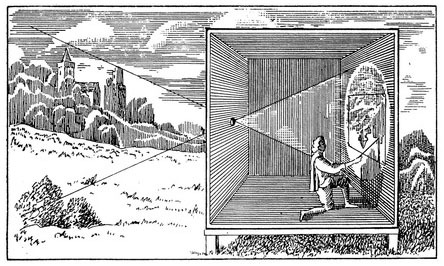
\includegraphics[width=.5\textwidth]{figures/chap2/photography/camera_obscura2}}
    \subfigure[]{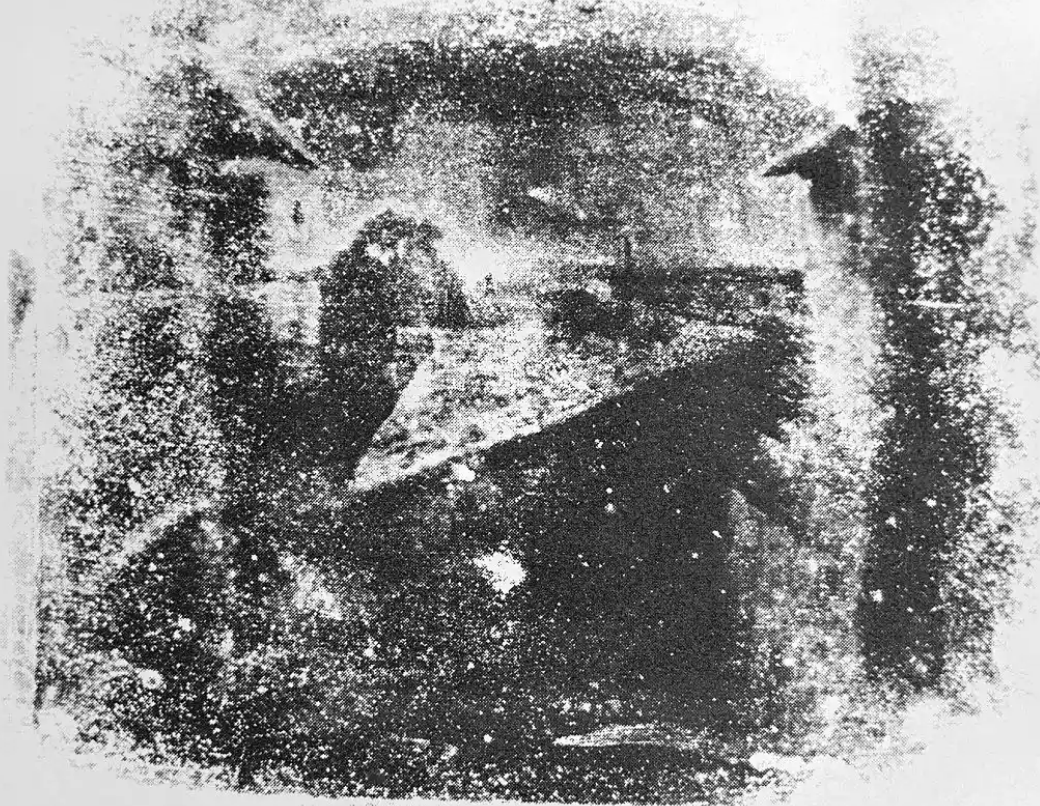
\includegraphics[width=.4\textwidth]{figures/chap2/photography/niepce}}
    \caption{(a) Camera obscura, (b) The first photograph}
    \label{c2:dark_room_photo}
\end{figure}

In the previous century, photography aside from invention became a new medium of communication, an art form and more affordable with Kodak's coloured film in 1936.

Photography as a form of art, arose from advancements in technology which enabled photographers to manipulate their image in order to form an artistic expression. Various equipment from different cameras, lenses, film and post processing techniques contributed to develop the photographer's individual genre and style of taking pictures. Since camera equipment became more modular and configurable, enabled the photographers to interact with them in order to create the picture as they wished, using techniques such as long exposures using low shutter speeds, create portraits using the different lenses or use the appropriate aperture value to put their subject in focus and make it stand-out while the background is blurred.

\subsection{Camera EXIF}

In the early film days, photographers were forced to write down the important information such aperture, shutter speed, date etc. in order to use this information in the lab during the film processsing and photo printing, a very painful process especially for new photographers.

In the era of digital photography, every modern digital camera is capable to store this information, along with all the relevant camera settings, built-in the photograph file. These settings can be utilised later in order to organise photographs, perform search and provide information about the particular camera gear and settings used.
Such metadata called EXIF(EXchangeable Image File Format) and can store a range of settings and parameters such as aperture, shutter speed, iso speed, focal length, camera model, lens type and much more.

It is much of important for a photographer who wish to find out of what ingredients a photo is made it is more than important to read this information; the latter may even be used by anyone who would like to share the information even in an image data set.

\subsection{Photography styles and camera settings}

A more experience photographer has a more firm grasp of which camera settings should be used when synthesizing a photo in order to produce the desired style. In general, there are numerous combinations to acquire the same level of illumination in a photo, but only a set of combinations to achieve a certain photography style characteristic. 
For example, in some cases an image with blurred subjects might be desired, when the synthesized frame and the camera settings are appropriately defined.
Such photography styles can be identified as long exposure shots, panning and bokeh as shown in Figure~\ref{c2:blurriness}. All of them share a similar characteristic, blurriness, but each one can only be achieved in different circumstances.

\begin{figure}[ht!]
    \centering  
    \subfigure[]{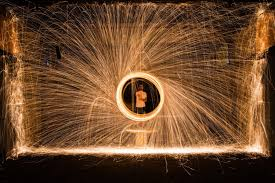
\includegraphics[width=.3\textwidth]{figures/chap2/photography/longexp}}
    \subfigure[]{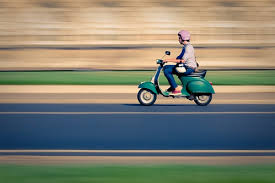
\includegraphics[width=.3\textwidth]{figures/chap2/photography/panning}}
    \subfigure[]{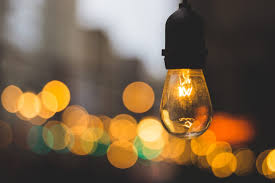
\includegraphics[width=.3\textwidth]{figures/chap2/photography/bokeh}}
    \caption{Photography styles with blurry characteristics: (a) Long Exposure, (b) Panning, (c)Bokeh}
    \label{c2:blurriness}
\end{figure}

For example, producing a long exposured image, cannot be easily done handheld and under the daylight. Since a photographer wishes to smooth out a particular object in the frame, camera should be placed steady and most import use a slow shutter speed setting. A slow shutter speed will let more amount of light to enter the medium and ``burn'' the sensor or the film in the correspondent surface that the image object is reflected.

On the other hand bokeh effect, relies mostly on the aperture and lens characteristics. It requires the viewer's attention to focus on a different area, that demonstrates an artificial perspective of three dimensional world in a two dimensional image. The technical part about how camera creates shallow or large depth of field, is basically a function of lens aperture, i.e. the variable opening that allows light to enter in the medium. When reduced to its smallest size, the aperture will create an image with a large depth of field, and when widened to its largest opening it will create a shallow depth of field.
Other factor that contribute to bokeh effect are proximity to the subject and focal length.
The term \textit{bokeh} can be defined as the effect of a smooth, out-of-focus background while the main image subject stays in focus.


As the camera became a more portable medium, several movements and famous photographers emerged, such as landscape photography, documentary, photojournalism, portrait, candid and more (Figure~\ref{c2:famous}).

Photography from artistic perspective, can be seen as a superficial dimension of reality. For the majority of the people, it is a subjective interpretation of an artificially constructed and arbitrary vision.
In the next section we attempt to approach the subjectivity term from the perspective of the domain of image aesthetics.

\begin{figure}[ht!]
    \centering  
    \subfigure[]{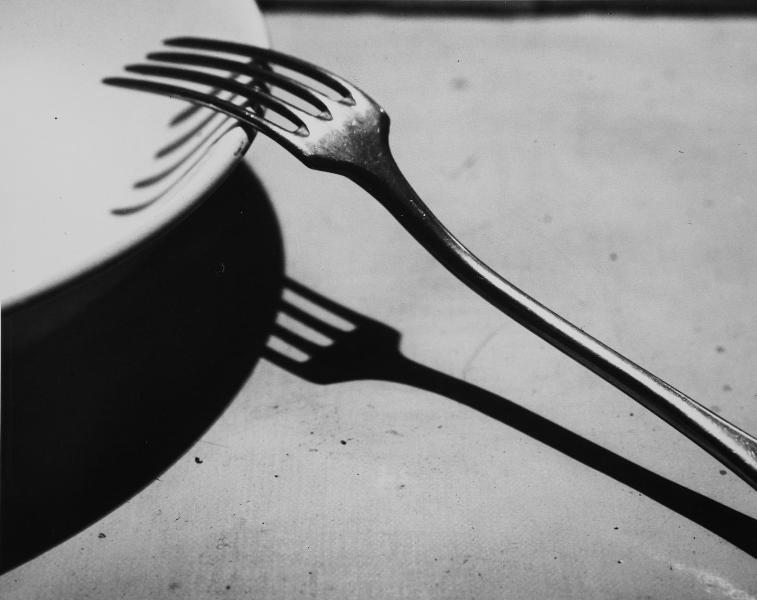
\includegraphics[width=.3\textwidth]{figures/chap2/photography/kertesz}}
    \subfigure[]{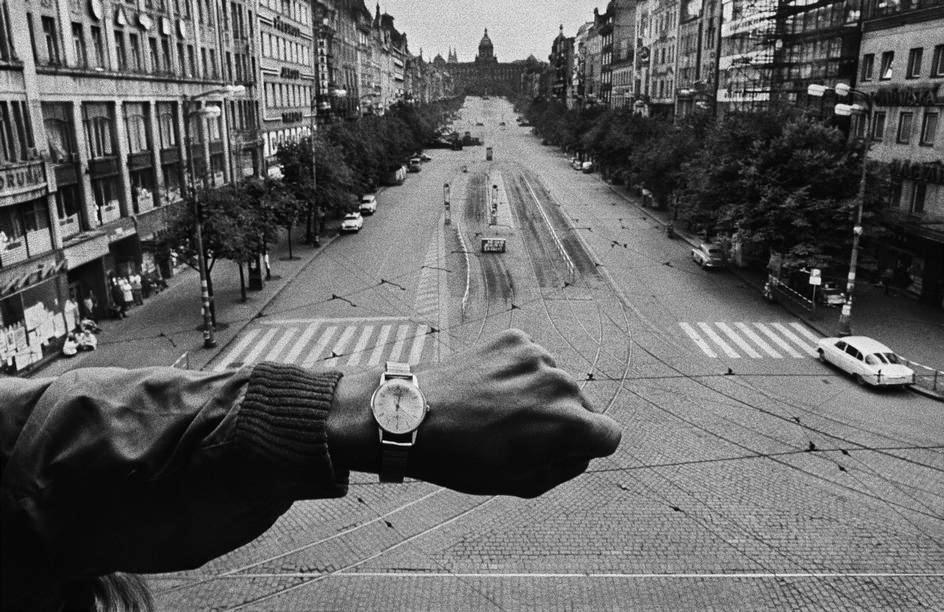
\includegraphics[width=.3\textwidth]{figures/chap2/photography/koudelka}}
    \subfigure[]{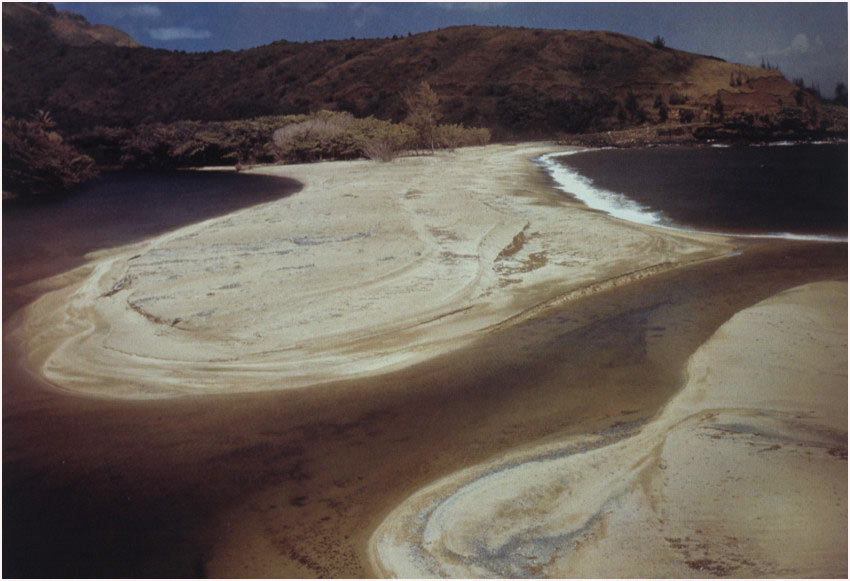
\includegraphics[width=.3\textwidth]{figures/chap2/photography/ansel_adams}}
    \caption{Famous photos with depth of field variations: (a) Andre Kertesz, (b) Josef Koudelka, (c)Ansel Adams}
    \label{c2:famous}
\end{figure}


%\chapter{Photography Style Analysis} \label{c4:intro}

\section{Aesthetics}
\label{c2:aesthetics}

The question in legitimacy of quantifying aesthetics was a subject of dispute between philosopher and art theorists and works as Jahanian's~\cite{jahanian2016quantifying} in 2016, attempted to provide a taxonomy map in order to quantify aesthetics shown in Figure~\ref{c2:aesthetics_taxonomy}.

\begin{figure}[ht!]
    \centering  
    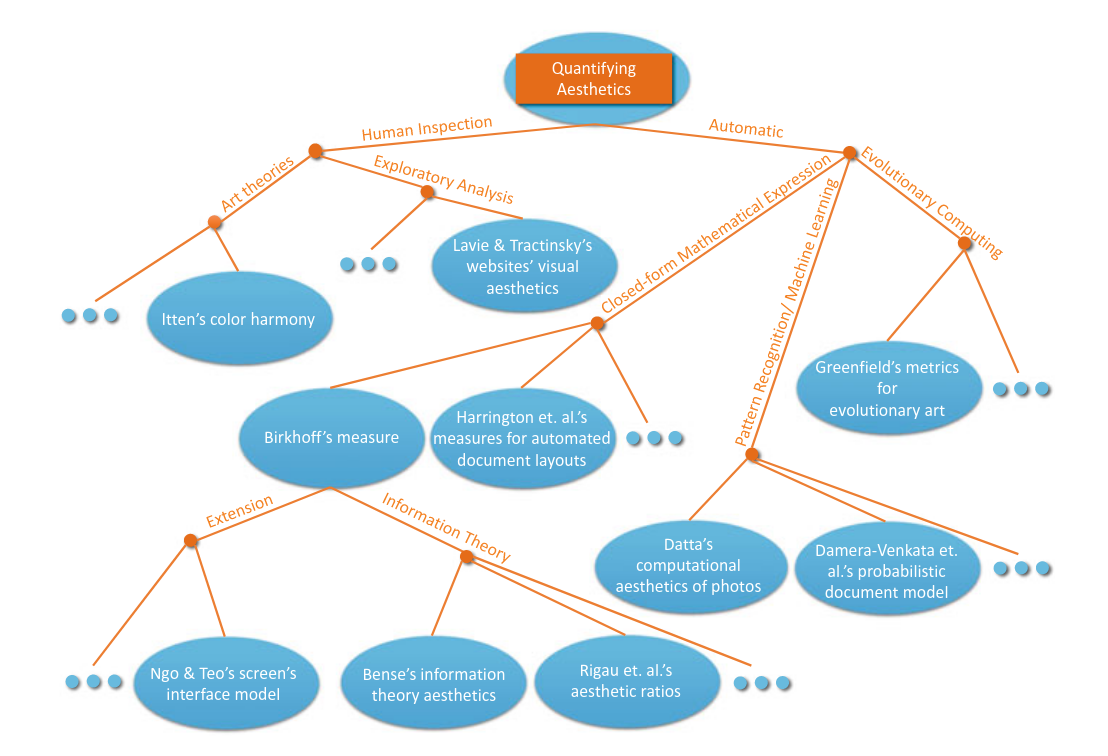
\includegraphics[width=.75\textwidth]{figures/chap2/aesthetics/taxonomy}
    \caption{Taxonomy of quantifying aesthetics}
    \label{c2:aesthetics_taxonomy}
\end{figure}

Of course, we are not the first who asked this question. In ancient years, Plato established a theory about natural and artistic beauty and the common reference that connects them, i.e., the imitation. Korsmeyer~\cite{korsmeyer1998aesthetics} summarized two opposite tenets about aesthetics. One by referring on Plato and Immanuel Kant that aesthetics is a matter of taste and the other by referring to Aristotle and Hans-Georg Gadamer, that aesthetics is a matter of cognition and learning. Yet, aesthetics is not only the study of beauty, but of taste, experience and judgement.

Based on the above taxonomy, we may find two main directions to approach it, either via human inspection or by automatic and evolutionary computations, able to measure aesthetics.


Regarding the human inspection approaches a well-known theory in visual design principles related to visual balance has been stated by a Gestalt psychologist and art theorist, Rudolf Arnheim~\cite{arnheim1960art},~\cite{marr1982vision}.
Specifically, he speculated that there exists a structural net, (Figure~\ref{c2:arnheim_net}) that contributes to a balanced spatial composition; this resembles much to the famous rule-of-thirds in photography, whereas Jahanian speculates that a good visual balance has Gaussian on the hot spots~\cite{jahanian2016deepcreativity}.

\begin{figure}[ht!]
    \centering  
    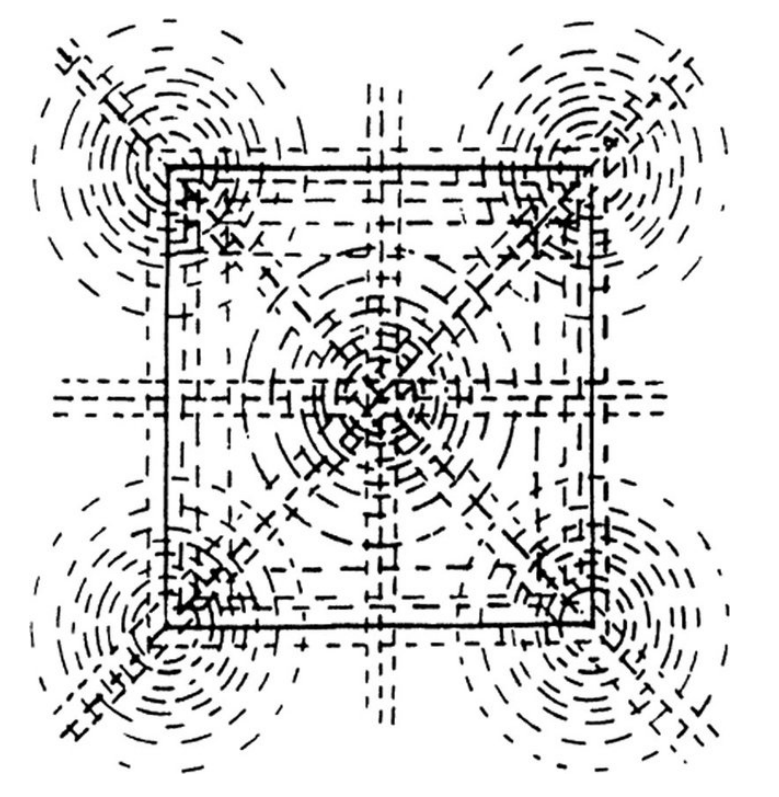
\includegraphics[width=.35\textwidth]{figures/chap2/aesthetics/arnheim_net}
    \caption{Arnheim's structural net}
    \label{c2:arnheim_net}
\end{figure}

\section{Image Aesthetics Quality Assessment(IAQA)}
\label{c2:sec_iaqa}

Image aesthetics can be defined as a subjective problem but over the latest decade image aesthetic quality assessment has demonstrated a tremendous success in variety of applications such advanced image search, retrieval and photo aesthetic enchancement.

IAQA aims to use computational techniques in order to simulate and understand human perception and cognition of the ``beauty'' and evaluate the ``beauty'' of the image.
Beauty can be described with several image aesthetic factors such content, object emphasis, light, colouring (black and white), depth of field (shallow/deep), composition (rule of thirds), motion, blur, etc.

Teaching a machine to assessing ``beauty'' is obviously a not-trivial task but recently artificial intelligence has made progress in these areas and the performance achieved in certain tasks can directly compared to humans'.
However, perceiving or creating ``beauty'' is still far away though IAQA is a crossroad for a diverse set of domains, such as computational cognition, computer vision, psychology, biology, fine arts and others~\cite{yang2019comprehensive}.

An interesting concept is the notion of \textit{aesthetic gap}~\cite{goree2021}, roughly analogous to the semantic gap in information retrieval, which separates low-level features of images like pixels and lines from high-level features like objects and symbols that humans observe in images.
Researchers have found that the feeling caused by a visual stimuli, is evoked by activations in distinct and specialized areas of the visual cortex.
Given that human perception follows a hierarchical path from the receptive field of our retina to the primal visual cortex~\cite{marr1982vision}, these activations can be categorized into the primal processing of visual stimuli inputs including colour, shapes, lines, orientation Figure~\ref{c2:vision}.

\begin{figure}[ht!]
    \centering  
    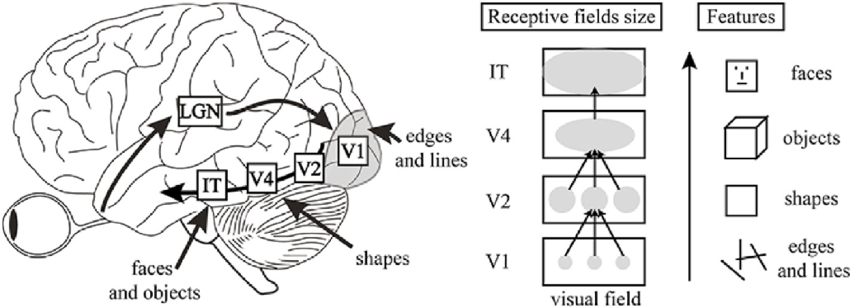
\includegraphics[width=.53\textwidth]{figures/chap2/aesthetics/human_vision}
    \caption{Perception of visual world as a hierarchical path.}
    \label{c2:vision}
\end{figure}

From the early research, IAQA does not follow the rule-based way but is treated as a data-driven learning problem. Therefore the construction of the data set is a key prerequisite to approach a certain problem.

Feature extraction techniques aim to extract high and low level features to describe and aesthetic image domain.
Traditional approaches use hand-crafted features to design specific photographic rules, image layout and objects and adopt classical machine learning algorithms to learn from those descriptions. Datta et al were determined to automatically learn from data which factors influence aesthetic value. Despite the problem ambiguity, there exist certain visual properties that make photographs more appealing than others~\cite{datta2006studying} as their concept derives from their data. They constructed a data set of 3000 images collected from \textit{photo.net} and used it to train decision trees and svms to classify images into high and low aesthetics categories based on feature variety(measures of colours, rule-of-thirds, image dimensions). However, due to the vagueness of certain photographic or art rules, hand-crafted features are often difficult to approximate them computationally.

An opposite approach for IAQA, this time from photo curation perspective proposed by Ke et al~\cite{ke2006design}, was based in computer vision rather than psychological aesthetics, by measuring image noise and degradation. Their method utilizes images and ratings from the photo challenge of \textit{DPChallenge.com}, which are used to extract features such edge and colour histograms and Fourier transformation based blur metrics in order to train a Naive Bayes classifier.

Later, a variety of other techniques emerged, proposing different image features like GIST or SIFT descriptors from Marchesotti et al.~\cite{marchesotti2011assessing} which argued on the non-exhaustive nature of hand-crafted features. The latter are heuristically generated and have shown generalization limitations in several problems and domains of application.


Based on a recent survey on computational aesthetic evaluation in visual art images~\cite{zhang2021comprehensive}, two research methods have been set, so far.
The first is based on conventional approaches such as the aforementioned ones, i.e., by using handcrafted features, while within the second 
aesthetic judgement is carried through deep learning techniques (Figure~\ref{c2:aesthetics_methods}). We shall provide further details regarding the latter in Section~\ref{c3:section_aesthetics_deep}.


\begin{figure}[h!]
    \centering  
    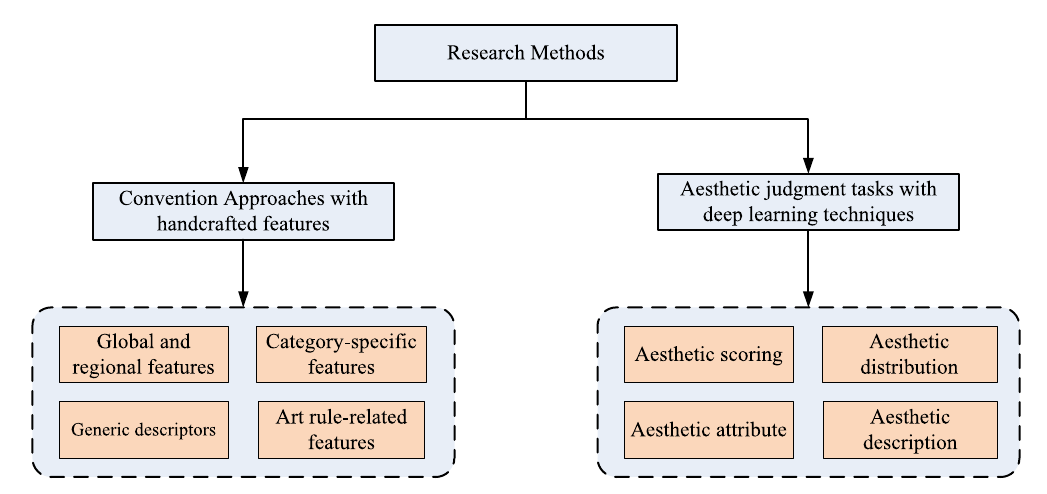
\includegraphics[width=.6\textwidth]{figures/chap2/aesthetics/methods}
    \caption{Research methods in aesthetic evaluation classification.}
    \label{c2:aesthetics_methods}
\end{figure}

So far we have covered the origins and latest developments in photography, analyzing popular photography styles and how they are related to general camera technical aspects. In addition, we have presented the philosophical and psychological background in aesthetics and traced the evolution of IAQA.

\newpage

% -------------------- Chapter 3 --------------------------------------- #
\chapter{Machine Learning}
\label{c3:intro}

\thispagestyle{empty}
\epigraph{\itshape ``Learn everything about something, and something about everything''}
{---Donald Knuth}

\section{Artificial Intelligence}

Undeniably the term of intelligence has gathered the attention of the most philosophical studies and discussions whether is something that exclusively exist in humans and animal or that it can be reproducible. If the latter is valid, how can we encode the human cognition in order to be understandable from a machine? Does it happen by simulating a small children's brain or let it learn by itself~\cite{turing1950computing}?
With the exponential growth of computational power the interest for automating certain procedures has increased. An effort to develop intelligent systems has assisted to create such applications that can aid to decision making in certain tasks. The term of \textit{Artificial Intelligence} has been established by $1956$ and some of the most remarkable real world applications are image recognition, natural language processing, driving assistance, art generation etc., have developed from self-trained systems without human interference. That particular domain of AI is called Machine Learning.


\section{Machine Learning}
\label{c3:ml}
In the era of big data we are surrounded of unlimited amounts of new data, generated each second. Billions of images from popular platforms like Instagram, Flickr and Unsplash to hundred of thousand hours of uploaded video, millions of eretail transactions per hour and so on.
This burst of data are subject to ubiquitous methods of data analysis which derive from machine learning techniques.
Machine learning, at its definition is a set of applied statistical methodologies that can learn from data upon a specific task and automatically discover patterns or learn to map data on some class.

Intuitively we take advantage of this knowledge to predict a pattern of unknown data or conduct inference by generating new information~\cite{murphy2012machine}.
Pattern recognition is linked with the automatic discovery of recurrences in data through the use of computer algorithms. The produced knowledge can assist to take actions, such decision making or classify data to different categories~\cite{bishop2006pattern}.

A more formal definition of Machine Learning is the following:
\begin{itemize}
 \item A \textit{computer program}, is a suitable to the task algorithm that has the capability of training.
 \item Experience \textit{E}, is the data set, that the algorithm is trained.
 \item The task \textit{T}, that the algorithm will learn to solve.
 \item The performance \textit{P}, the measurement that will be used in order to monitor the algorithm on how well performs on the task.
\end{itemize}


\subsection{Learning Tasks}

Machine learning diverges from the classical rule-based approach of an algorithm which is a standard procedure that one can explicitly define. On the other hand, an ML algorithm is not an algorithmic process but a set of methods that are not programmed but trained on sets of data.

Most of ML methods, fall into 3 broad categories:
\begin{itemize}
 \item \textbf{Supervised Learning}, the algorithm is trained on associations of the input data to  corresponded labels.
 \item \textbf{Unsupervised Learning}, the algorithm is trained without human supervision.
 \item \textbf{Reinforcement Learning}, a less commonly used type of learning which works as a rewarding/punishing system upon an actor~\cite{sutton2018reinforcement}, but is beyond the scope of this work.
\end{itemize}

In this thesis, we focus on supervised learning to solve a non-trivial task, in the context of image aesthetics.

To begin with, consider the example of handwritten digit recognition illustrated in Figure~\ref{c3:mnist}. Each digit is represented by a 28 $\times$ 28 pixel gray-scale image and so it can represented by a 1-d vector $x$ of 784 size. The task is to build a model that will take as input such a vector $x$ and will produce a label identified by the digit number 0,\dots,9 to the output.

\begin{figure}[h!]
    \centering  
    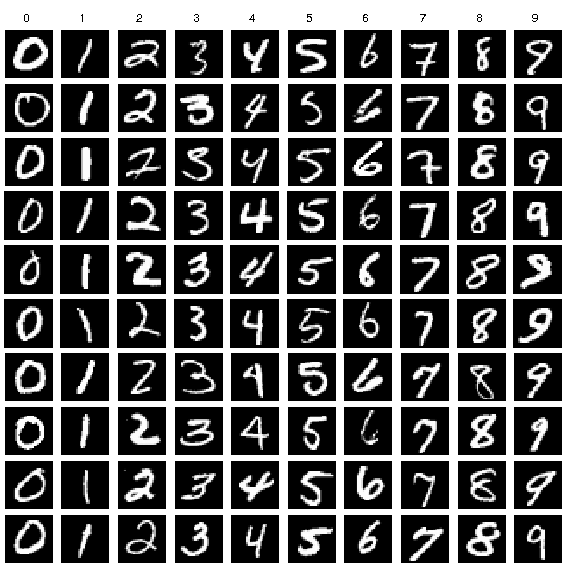
\includegraphics[width=.4\textwidth]{figures/chap3/ml/mnist}
    \caption{Hand-written digits data set}
    \label{c3:mnist}
\end{figure}

The task is non trivial at hand due to the variety of handwritten digits and employing a rule-based solution using handcrafted rules and classical image processing techniques will lead to an explosive amount of rules and so forth will give poor results.
By adopting a machine learning approach, we can create a large set of $N$ digits namely a \textit{training set}, of samples $X = \{x_1,\dots,x_N \}$ and target vectors $y = \{y_1,\dots,y_N \}$ and use it to train an adaptive model by optimizing each parameters in order to maximize classification performance.
Typically we are feeding the machine learning model with pairs of:
\begin{enumerate}
 \item \textbf{samples} $x$ expressed by the digit vector and 
 \item \textbf{target} vectors $t$, which represent the identity of the corresponded digit
\end{enumerate}

A target vector, denoted as \textbf{label}, is produced from a human input, known as annotation process.
During the \textit{training phase} model is determined to learn the \textit{training data}.

More specifically, it learns to map the samples on the associated targets and by the end of training it is expected to identify unknown samples which hasn't seen before, namely, the \textit{test} set. The ability to recognize an unknown digit falls to the problem of \textit{generalization}~\cite{mitchell1986explanation} which is a practical problem in all applications.
For the most applications, input samples are subject to typical \textit{preprocessing} steps in order to transform them into a new parameter space to ease and accelerate training and learning. For example in the case of hand written images, a gray-scale image is represented in 8-bit ranges from 0-255 integer values. Rescaling the values into 0-1 scale, will help to reduce the variability of the data it make it much easier for the classifier to distinguish between the classes. The preprocessing stage can be sometimes called \textit{feature extraction}.
In most of the tasks, where the raw data are multi and high dimensional, preprocessing step is essential, otherwise it will be computationally infeasible for the machine learning model to converge.
Such tasks as the one described above fall into the domain of \textbf{supervised learning} problems and belong to a broader family of problems those, of \textit{Image Classification}. In such a task a model \textit{g} also called \textit{estimator}, will be trained and learn to map an input vector sample, to a certain class, from a finite number of available classes $x_i \rightarrow y_i$.

Practically, a perfect association can never be made, because of the model's incapability to describe complicated mappings or due to the descriptive information of the features. Thus, we state that a model \textit{g} \textbf{predicts} or \textbf{infers} hypothesis $\hat{y}_i$ for the sample $x_i$, as $\hat{y}_i = g(x_i)$.

On the other hand assuming that the desired output could be a continuous variable, the task is called \textit{regression}. An example of regression problem could be the prediction of a house price given an input feature vector that represents e.g. a residential area, size of house etc.

In many cases where the human input and target labels are unavailable, the training data consist only of a set of input samples \textbf{x}. Such problems belong to the category of instance-based learning or \textit{unsupervised learning}. Such tasks can be \textit{clustering} where the algorithm discovers groups of similar instances within the training samples or to determine the distribution of data and discover latent representations from high dimensional input projected to a smaller number of dimensions for the purpose of \textit{visualisation}. An example of a visualised clustering application on the same data set is illustrated in Figure~\ref{c3:clustering}.

\begin{figure}[h!]
    \centering  
    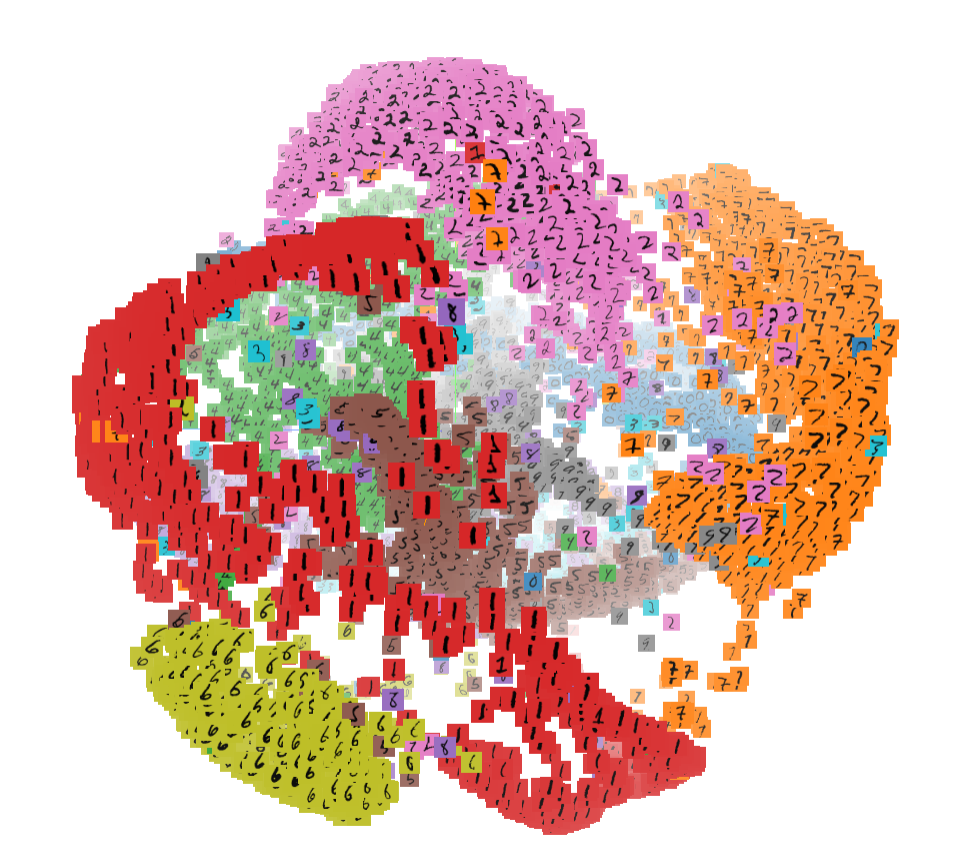
\includegraphics[width=.5\textwidth]{figures/chap3/ml/clusters}
    \caption{Hand-written digits data set visualised in clusters}
    \label{c3:clustering}
\end{figure}

\section{Deep Learning}

A sub-domain of machine learning, known as Deep Learning (DL), has substantial growth in many types of machine learning systems over the latest years. Conventional machine learning techniques are limited to their ability to process the data at its natural form~\cite{lecun2015deep}. Machine learning systems are relying to careful feature engineering and sophisticated feature extraction techniques with considerable domain expertise, in order to feed a classifier with data and produce a result.
Deep learning methods are representation learning methods able to fed with unstructured data (images, text, voice, etc.) without any prior handcrafted feature extraction technique. It utilises of non-linear activated modules able to transform the data directly from the input, into high-level feature representations. Compositing multiple modules we are able to learn very complex functions due to the hierarchical structure of the network. A deep neural network is illustrated in Figure~\ref{c3:dl}.

\begin{figure}[h!]
    \centering  
    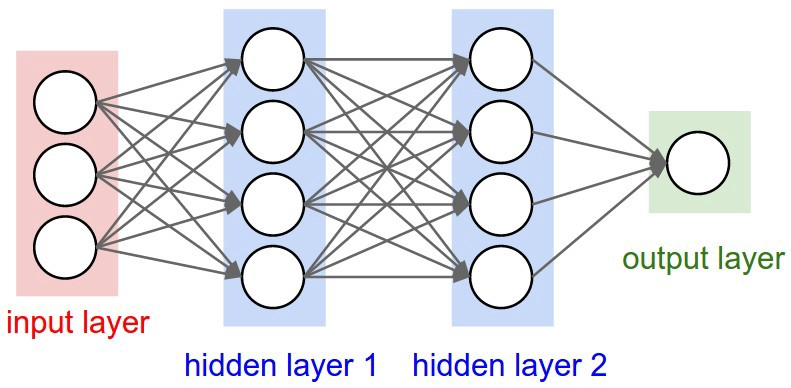
\includegraphics[width=.6\textwidth]{figures/chap3/ml/dl}
    \caption{Deep neural network}
    \label{c3:dl}
\end{figure}

This has led to groundbreaking advances in the domain of \textit{Computer Vision} and \textit{Natural Language Processing} as one is able to process huge amounts of data and solve complicated problems that were unable to get solved by the AI community for many years.

Deep learning turned out to be very good at discovering complex structure in high-dimensional data and consequently deep learning models are successfully deployed and support real life applications in domains of science and business products.

\section{Computer Vision}

From the early 70s the field of computer vision started as an attempt to shed some light in the open problem of visual perception. Pioneers of their time such Winston~\cite{winston1975psychology} attempted to set a frame on the global scene understanding, Barrow~\cite{barrow1981interpreting}, proposed an approach to understand the fundamental importance of surface perception interpreting line drawing and Marr~\cite{marr1982vision} as discussed in Section~\ref{c2:aesthetics}, introduced the notion of a visual processing system summarised in the three levels of computational theory, representation and algorithms and hardware implementation.
In 80s, more sophisticated techniques have emerged to perform quantitative image and scene analysis for better edge and contour detection Canny~\cite{canny1986computational}.
In 1990s, a burst in more integrated applications was recorded such in image segmentation by Haralinck~\cite{haralick1985image} and in image restoration by Banham~\cite{banham1997digital}.
In the decade of 2000, the exponential growth in computational photography increased the demand for computational techniques for the every day photography. For example image stitching~\cite{brown2007automatic} to create photographic panoramas, automatic exposure bracketing into a composition of high dynamic range scene~\cite{reinhard2010high}, tone mapping to effectively correct the image gamut and prevent from burned or darken images~\cite{durand2002fast}, super resolution and blur removal~\cite{baker2002limits}, vignette and exposure calibration~\cite{goldman2010vignette}.

The problem we are going to tackle in this work, lies in the domain of computer vision (CV). Computer vision tries to describe the natural world in images and reconstruct its properties, such shape, illumination and colour distributions~\cite{szeliski2010computer}.

Nowadays, we are interacting with computer vision applications to a wide variety of solved problems such medical imaging, optical character recognition (OCR), pose estimation, photogrammetry, motion capture, face and object detection, image stitching, image filtering and many more.

\begin{figure}[h!]
    \centering  
    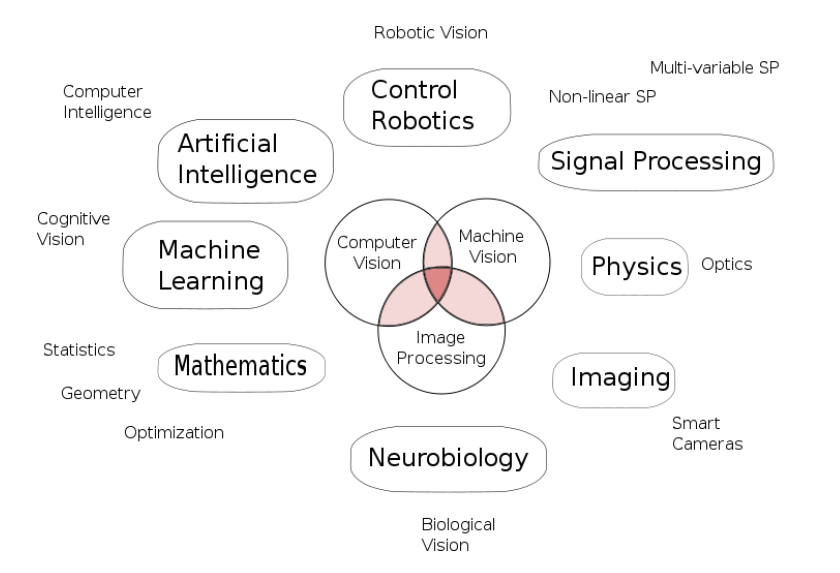
\includegraphics[width=.6\textwidth]{figures/chap3/cv/cv}
    \caption{Computer vision map}
    \label{c3:cv}
\end{figure}

\begin{figure}[ht!]
    \centering  
    \subfigure[]{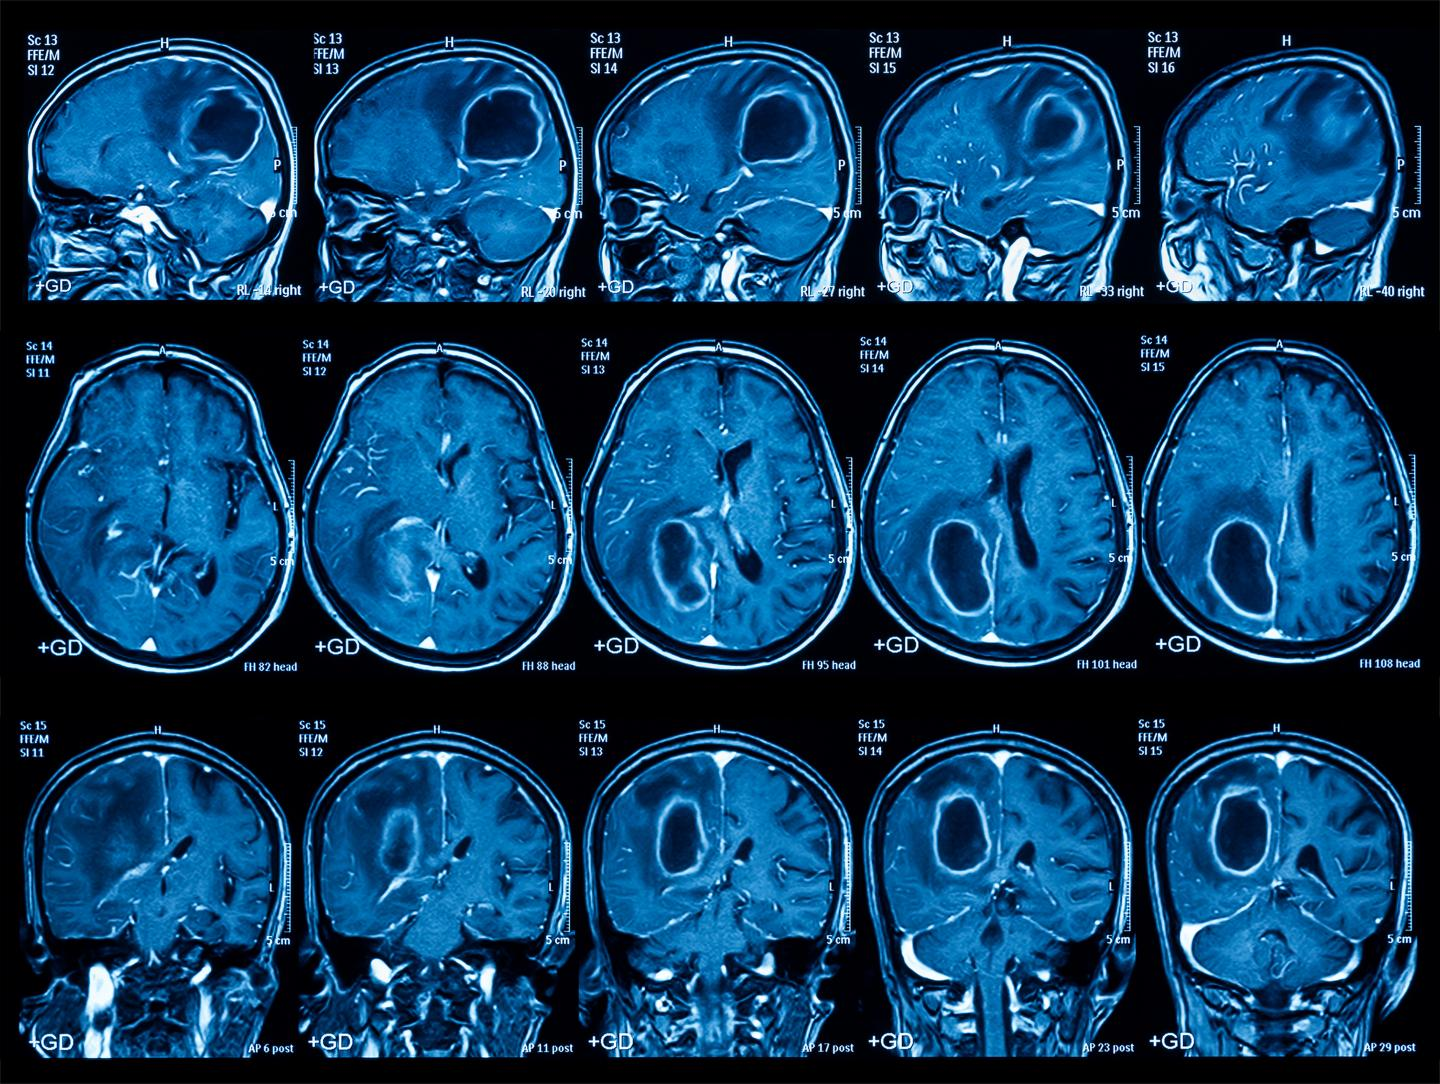
\includegraphics[width=.3\textwidth]{figures/chap3/cv/medical}}
    \subfigure[]{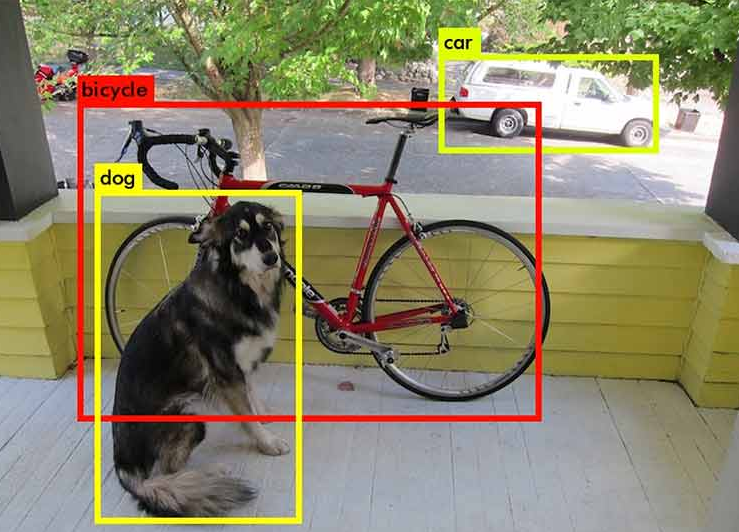
\includegraphics[width=.3\textwidth]{figures/chap3/cv/od}}
    \subfigure[]{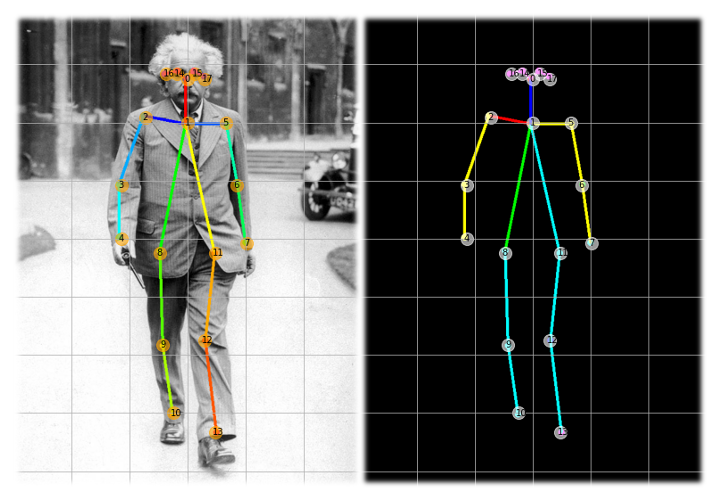
\includegraphics[width=.3\textwidth]{figures/chap3/cv/pose}}
    \subfigure[]{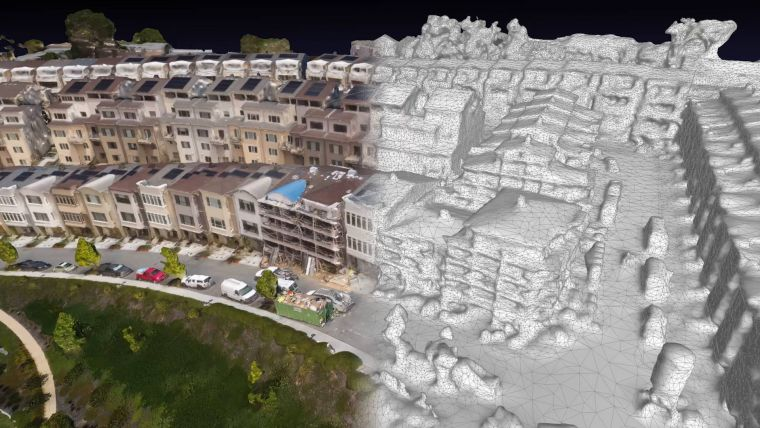
\includegraphics[width=.4\textwidth]{figures/chap3/cv/photogrametry}}
    \subfigure[]{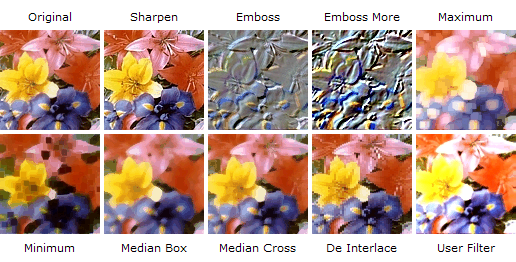
\includegraphics[width=.5\textwidth]{figures/chap3/cv/filters}}
    \caption{Computer vision applications: (a) Medical imaging, (b) object detection, (c) Pose estimation, (d) Photogrametry, (e) Image filtering}
    \label{c3:cv_apps}
\end{figure}

\section{Neural Networks}

Neural networks (NN) is a type of model that can be utilised to solve efficiently classification problems. The basic building unit that constructs a neural network is called \textit{Neuron} or \textit{Perceptron}~\cite{rosenblatt1958perceptron}.

A neuron is able to perform two operations: a linear (or affine) transformation to its input and a non-linear function application to the output. A neuron is described from the next equation:
\begin{ceqn}
\label{c3:perceptron_eq}
\begin{align}
    z = f(w \cdot x + b)
\end{align}
\end{ceqn}
In the above equation~\ref{c3:perceptron_eq}, the input is represented as a vector $x \in \mathbb{R}$ such as an image or audio. This input is multiplied by the weight matrix $w \in \mathbb{R}$ which coefficient is a tunable parameter bias $b \in \mathbb{R}$.
These operations consist the linear transformation of the Perceptron. 
Then, every component of the result vector is passed through a non-linear function \textit{f} which is called \textit{activation function}.
The most popular activation functions that are used thoroughly are the sigmoid, tanh, ReLU and softmax. More for the activation functions is discussed in Section~\ref{c3:activation_functions_sec}.

When we say that a network learns, it means that in the training phase the neuron parameters \textit{w} and \textit{b} are being adapted in respect of the network output. A neuron is presented in Figure~\ref{c3:perceptron}.

\begin{figure}[h!]
    \centering  
    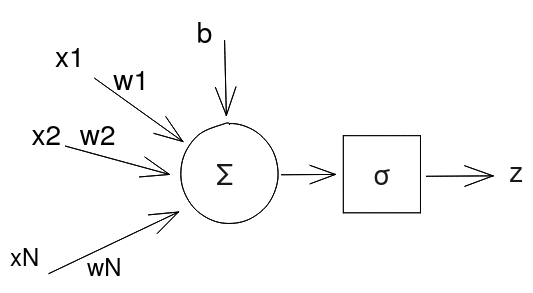
\includegraphics[width=.5\textwidth]{figures/chap3/ml/neuron}
    \caption{A representation of a neuron. N number of \textit{x} input vectors are multiplied with the corresponded weights \textit{w} with added bias constant \textit{b}. The outcome activates a non-linear function.}
    \label{c3:perceptron}
\end{figure}

\subsection{Multi-layer Perceptron}

A typical neural network consists of multiple layers; the output of one is the input of the other in the next layer. In such hierarchical fashion, the network is able to estimate non-linear functions. 
Repeating this process, it becomes a multi-layer percepton (MLP) network as it is shown in Figure~\ref{c3:mlp}.

\begin{figure}[h!]
    \centering  
    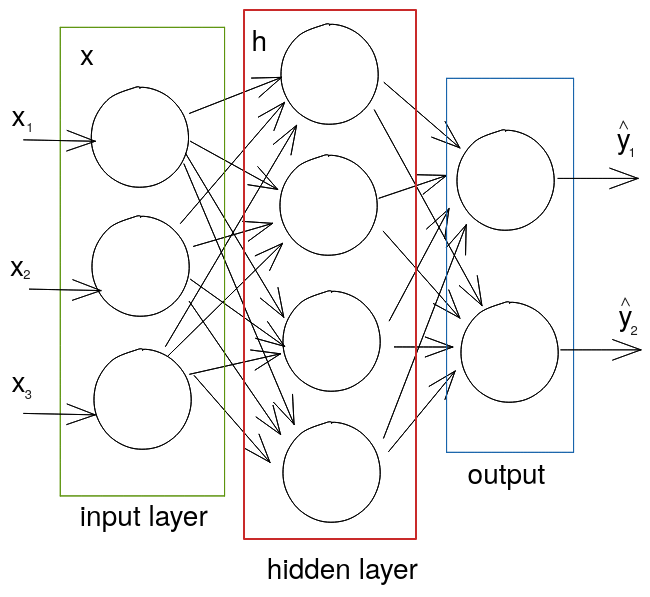
\includegraphics[width=.5\textwidth]{figures/chap3/ml/mlp}
    \caption{A Multi-layer perceptron network having a general feed-forward topology.}
    \label{c3:mlp}
\end{figure}


\section{Training a model}

The standard training procedure applies to any kind of neural network architecture. A simplified case, is a simple shallow network as the above and can be described from the following equation:

\begin{ceqn}
\label{c3:perceptron_mlp_equation}
\begin{align}
    \hat{y} = f(W \cdot x + b),~ W \in \mathbb{R}^{M\times C}, x \in \mathbb{R}^{M}, b \in \mathbb{R}^{C}
\end{align}
\end{ceqn}


Where \textit{M} in the cardinality of input and \textit{C} the number of classes. The input samples constitute a vector of \textit{M} number of values, $x = \{x_{i}^{1}, \dots, x_{i}^{M} \}$
The label value takes the corresponded value of class, as $y_i \in \{ 1, \dots,\text{C} \}$. The output of the network $\hat{y}$ is the one that we are looking for to approach in correspondence to the real label value as it is estimated from the type of activation function in the last output layer.


\subsection{Activation functions}
\label{c3:activation_functions_sec}

Fitting a multilayer neural network requires the choice of an activation function and a network architecture. During the forward pass in training process, the output of a neuron is passed to the next layer only if activated a certain function is applied to the output. While the type of the function is determined from the task to be solved where are going to discuss the activation functions that we have used in our work.
Traditionally in neural networks, sigmoidal activations functions were employed but for a deep neural network (dnn) there is a computational advantage when using a non-sigmoidal rectified linear unit (ReLU)~\cite{schmidt2020nonparametric}.

For classification problems, the ReLU is suggested over a sigmoidal~\cite{glorot2011deep} for image and also text based problems. The ReLU handles better the problematic output of sigmoid function and vanishing gradient phenomenon may occur during the backpropagation. Figure~\ref{c3:activation_functions} illustrates the aforementioned activation functions and the corresponded equation are provided in~\ref{c3:sigmoid_eq},~\ref{c3:relu_eq}.
\begin{ceqn}
\label{c3:sigmoid_eq}
\begin{align}
    \sigma(x) = \frac{1}{1+e^{-x}}
\end{align}
\end{ceqn}

\begin{ceqn}
\label{c3:relu_eq}
\begin{align}
  \text{ReLU}(x) = \text{max}(0,x)
\end{align}
\end{ceqn}

\begin{figure}[ht!]
    \centering  
    \subfigure[]{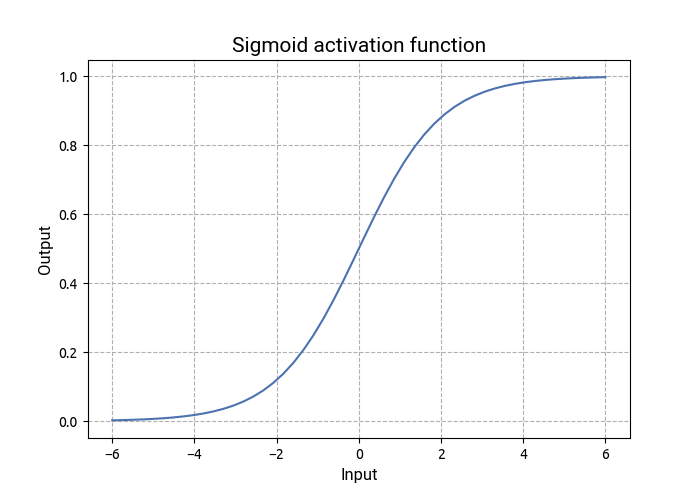
\includegraphics[width=.45\textwidth]{figures/chap3/ml/sigmoid}}
    \subfigure[]{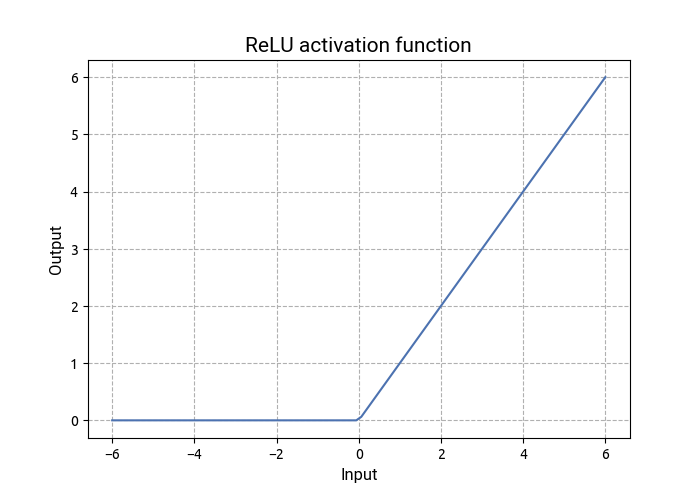
\includegraphics[width=.45\textwidth]{figures/chap3/ml/relu}}
    \caption{Activation functions: (a) Sigmoid, (b) ReLU }
    \label{c3:activation_functions}
\end{figure}

Additionally, concerning the network output the activation function is determined based on the problem at hand. The main problems are the following:

\begin{itemize}
 \item \textbf{Linear Regression}, where the predicted variable has continuous values, so $\hat{y} \in \mathbb{R}$. This task does not require an activation function.
 \item \textbf{Logistic Regression or Classification}, the predicted variable takes a nominal value of the given classes \textit{C}, so $\hat{y} \in \mathbb{N}$. In this case, the \textit{softmax} function is used.
\end{itemize}

Softmax is declared by the equation:

\begin{ceqn}
\label{c3:softmasx_eq}
\begin{align}
  \text{softmax}(z)_i = \frac{e^{z_i}}{\sum_{j=1}^{C} e^{z_j}}
\end{align}
\end{ceqn}

Intuitively, softmax normalize the \textit{z} input into a probability distribution that each output is a posterior probability given a value in the interval $[0,1]$.

\begin{figure}[h!]
    \centering  
    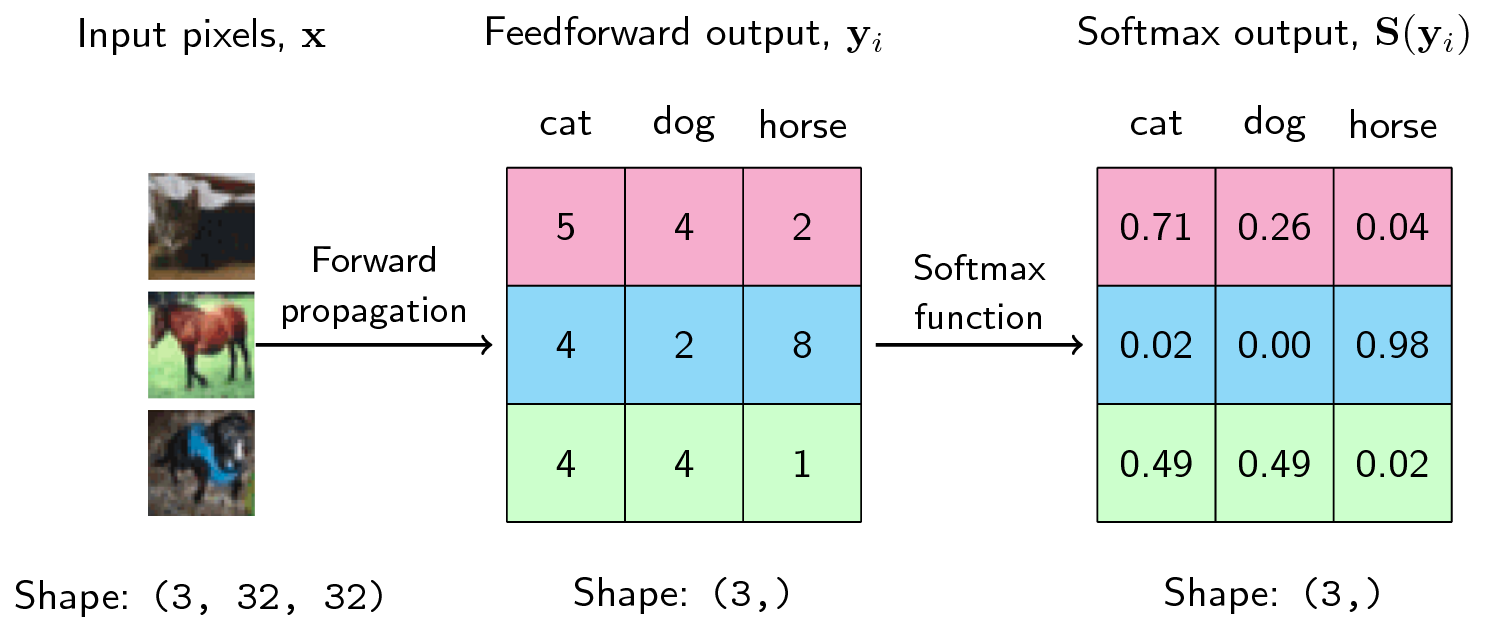
\includegraphics[width=.7\textwidth]{figures/chap3/ml/softmax}
    \caption{Intuitive example of the softmax function. In left the input data for each class. In right the softmax output aggregating to 1.}
    \label{c3:softmax}
\end{figure}

\subsection{Loss/Cost function}

When the forward pass is completed the network output $\hat{y}$ should be compared with the real values (groundtruth) in order to measure the discrepancy. Based on the definition from Section~\ref{c3:ml}, measuring the error between the prediction and the groundtruth, informs us of how good or bad the network performs during the training process. To measure the error, a \textit{loss} function will be utilised.

For \textit{linear regression} type problems, where the predicted $\hat{y}$ and groundtruth $y$ are continuous variables, we use the Mean Squared Error (MSE).

\begin{ceqn}
\label{c3:mse_eq}
\begin{align}
  \text{MSE}(y, \hat{y}) = \sum_{i=1}^{N} (y_i, \hat{y_i})^2
\end{align}
\end{ceqn}

MSE loss function is minimized when the predicted value $\hat{y}$ is as close enough to the groundtruth $y$.

For \textit{classification} problems the groundtruth values $y$ are encoded to vectors in length of the number of classes. This encoding is known as \textit{one-hot} encoding. More specifically each label $y_i$ is a binary vector, where its digit represent a class \textit{C}. A position with 1 in the vector, denotes the relative class. An example of an one-hot encoded vector is shown bellow.

The available class labels representing three digits are \textit{one, two} and \textit{three}.
\begin{ceqn}
\label{c3:one_hot_example}
\begin{align*}
  \text{digit} \rightarrow \text{(one two three)}
\end{align*}
\end{ceqn}

Each digit's label is one-hoe encoded in a binary vector.

\begin{ceqn}
\begin{align*}
        \begin{pmatrix} one \\ two \\ three \end{pmatrix} & \rightarrow \begin{pmatrix} 0 & 0 & 1 \\ 0 & 1 & 0 \\ 1 & 0 & 0 \end{pmatrix}
\end{align*}  
\end{ceqn}
\\

The loss function that is used in classification problems is called \textit{categorical cross-entropy}.

\begin{ceqn}
\begin{align}
  \text{J}(y, \hat{y}) = -\sum_{i=1}^{N} y_i \cdot \log \hat{y_i}
\end{align}  
\end{ceqn}
\\

The minimization of the loss function equals to the maximization of the posterior prediction that a network gives for a certain input $x_i$ to correspond to a class label $y_i$. In other words, we are looking for the \textit{Maximum Likelihood Estimation} (MLE).

\subsection{Learning process}

Now that we have defined most of the essential components of a neural network, we are going to discuss about the learning process.
Learning process is as iterative method that is carried over in \textit{epochs} and stops when a criteria is met. Our true objective is to find those network's parameters weights $W$ and biases $b$ that minimize the error of the cost function as intuitively presented in Figure~\ref{c3:wnb}.

\begin{figure}[h!]
    \centering  
    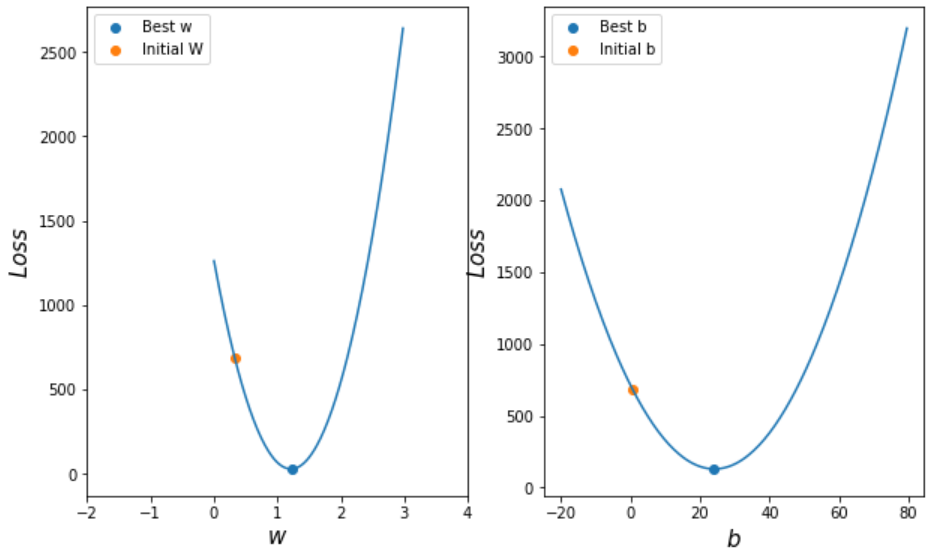
\includegraphics[width=.8\textwidth]{figures/chap3/ml/wnb}
    \caption{Initial and best weights and biases values hitting a local minima}
    \label{c3:wnb}
\end{figure}


During the forward pass, a sample is passed through the network of neurons until the final layer which outputs a posterior probability and the loss function calculates the error between the prediction and the groundtruth. Given the discrepancy, we need to inform the network about the error and adapt its parameters and start over. The problem is considered an optimization process and can be solved utilising a method called \textit{gradient descent}. By computing the gradients of the loss function with respect to each of the parameters $W$ and $b$ we are calculating the slope of the function to be approximated, at the current positition. The slope shows the direction that will follow in order to reduce to cost function's value.
For example, we calculate the weight's matrix $W_i$ as follows:

\begin{ceqn}
\begin{align}
    \nabla_{W_i}\text{J}(y, \hat{y}) = \frac{\partial\text{J}(y, \hat{y})}{\partial W_i}
\end{align}  
\end{ceqn}

and the updated value for the next epoch is given by:

\begin{ceqn}
\begin{align}
  W_{i}^{e+1} \leftarrow W_{i}^{e} - \lambda \cdot \frac{\partial\text{J}(y, \hat{y})}{\partial W_{i}^{e}}
\end{align}  
\end{ceqn}

where $\lambda$ is the \textit{learning rate} hyperparameter and dictates the magnitude of the update. Smaller values will require more steps for a network to converge, larger values might lose the minima and the network might never converge.
The above method can be consider a criterion to be met and the procedure is referred as \textit{training process} or \textit{fitting} while each learning cycle is referred as an \textit{epoch}.

For network architectures with multiple layers, a chain rule is applied to calculate the gradients of the layers next.

\begin{ceqn}
\begin{align}
    \frac{\partial\text{J}(y, \hat{y})}{\partial W_{i}} = \frac{\partial\text{J}(y, \hat{y})}{\partial z_{L-1}} \cdot \frac{\partial z_{L-1}}{\partial z_{L-2}} \cdot  \ldots  \cdot \frac{\partial z_{i}}{\partial W_{i}}
\end{align}  
\end{ceqn}
\\
For computational reasons, layers are updated backwards from the latter to the former, this operation is referred as \textit{backpropagation}.

\subsection{Optimization}

Overall, the main steps of machine learning are to build a model hypothesis (\textbf{M}), define the objective function (\textbf{J}) and solve the maximum or minimum of the objective function to determine the parameters (\textbf{w,b}) of the model.
The first two are the modelling problems of machine learning and the latter is to train the model by an optimization algorithm (optimizer).

An optimizer in deep neural networks is involved in many contexts. The simplest form used is the \textit{gradient descent} of the previous section.
An optimizer in general focuses on to find the parameters \textbf{$\theta$} of a neural network that significantly reduce a cost function $J(\theta)$~\cite{Goodfellow2016}.

\textit{Gradient descent} follows a global optimal solution, where all training samples \textit{N} are involved towards the calculation of the cost and when the objective function is convex like, similar to Figure~\ref{c3:wnb}.
Because this problem is very important and can become very expensive in applications with hundreds or millions trainable parameters that a specialized set of optimization techniques have been developed for solving it.

A variant of the above technique called \textit{Stochastic Gradient Descent} (SGD) uses a random sample \textit{i} rather than all samples, to update the gradient per iteration. That particular sampled is called \textbf{batch} while the cardinality of samples included in batch define the \textbf{batch size}.
\begin{ceqn}
\begin{align}
 \theta^{i+1} = \theta^i - \lambda \cdot \partial_{\theta^i} J(y_b,\hat{y_b}), b \subset N
\end{align}
\label{c3:eq_sgd}
\end{ceqn}
For every batch \textit{b} on iteration \textit{i}, SGD calculates the cost and updates model parameters in Equation~\ref{c3:eq_sgd}. After N/b iterations, when all samples \textit{N} have passed ones from SGD an \textit{epoch} is completed.

The main advantage of this method is that it does not require to load the entire set in memory, but only a batch. This technique enable training feasible for larger volume of data sets and despite the more iterations needed, this method is faster as since less computational time is less. It is also observed that SGD has regularization effects in training, as it mitigates overfitting~\cite{sun2019survey}.

Other successful variants of SGD, extend the equation with \textit{momentum}, an idea that derived from the mechanics of physics and preserves the influence of the previous update direction on the next iteration to a certain degree developing a mechanism to overcome local minima.
\begin{ceqn}
\begin{align}
 u^i = \lambda \cdot \partial_{\theta^i} J(y_b,\hat{y_b}) + \gamma u^{i-1}
\end{align}
\label{c3:eq_sgd_momentum}
\end{ceqn}
Momentum term is the $\gamma u^{i-1}$. If the update of the previous iteration  $u^{i-1}$ is high, then it will increase also the current iteration and thus the update is more increased. 
Other modern optimizers~\cite{kingma2014adam},~\cite{zeiler2012adadelta},~\cite{ duchi2011adaptive},~\cite{dozat2016incorporating}, utilise the above concept to optimize the momentum calculation and contribute to smoother gradient descent progression and ensure that training will converge.

\subsection{Bias and Variance}

Bias and variance are two types of errors that a classifier is subjected to make.
\textit{Bias} occurs from the false estimations during training. In neural networks, bias may arise when the network complexity is very simple, namely it does not have the capacity to learn more complex representation of the input \textit{X} related the label \textit{y}. For example, if the task is complex and a low capacity or complexity network is used, high bias is expected to occur. High bias is also referred as underfitting. An example of classifier with high bias is visualized in Figure~\ref{c3:fig_bias}.

\begin{figure}[h!]
    \centering  
    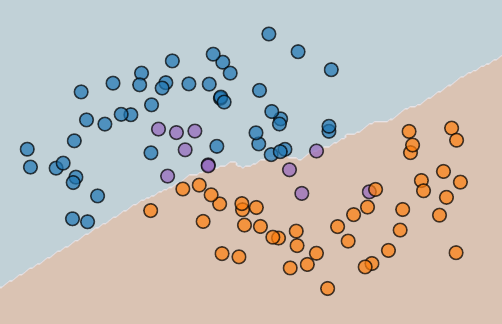
\includegraphics[width=.7\textwidth]{figures/chap3/ml/bias}
    \caption{Example of a classifier with high bias. Circles are the samples \textit{X}. Blue and orange are the corresponded class that a sample is assigned, while in purple are the false predictions. A linear classifier has not the ability to learn the non-linear complexity of that particular data set.}
    \label{c3:fig_bias}
\end{figure}

\textit{Variance} is a concept related to bias which derives from the classifier's sensitivity in minor input changes. In practice, means that the classifier can capture random variation in input such noise or from random behavior in the learning algorithm itself, such random initial weights~\cite{dietterich1995machine}.  An example of classifier with high variance is visualized in Figure~\ref{c3:fig_variance}.

\begin{figure}[h!]
    \centering  
    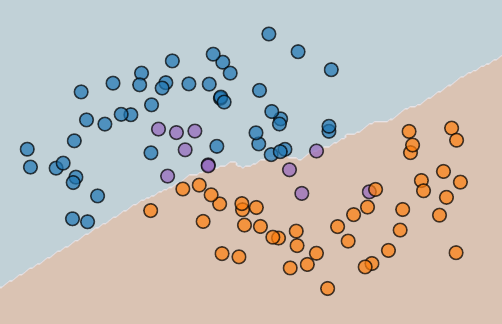
\includegraphics[width=.7\textwidth]{figures/chap3/ml/bias}
    \caption{Example of a classifier with high variance. The decision line is overfitted on the samples as the classifier has learned perfectly the data set. That will cause issues in task generalisation.}
    \label{c3:fig_variance}
\end{figure}

\subsection{Objective performance evaluation}

To prevent classifier from overfitting and ensure the proper network generalisation, we ``hide'' completely a portion of the data from the classifier during training and use it only for evaluation. In this way, we divide the data set \textit{X}, in two subsets: \textit{train set} $X_{train}$ and \textit{test set} $X_{test}$ as in Figure~\ref{c3:fig_train_test}.

\begin{figure}[h!]
    \centering  
    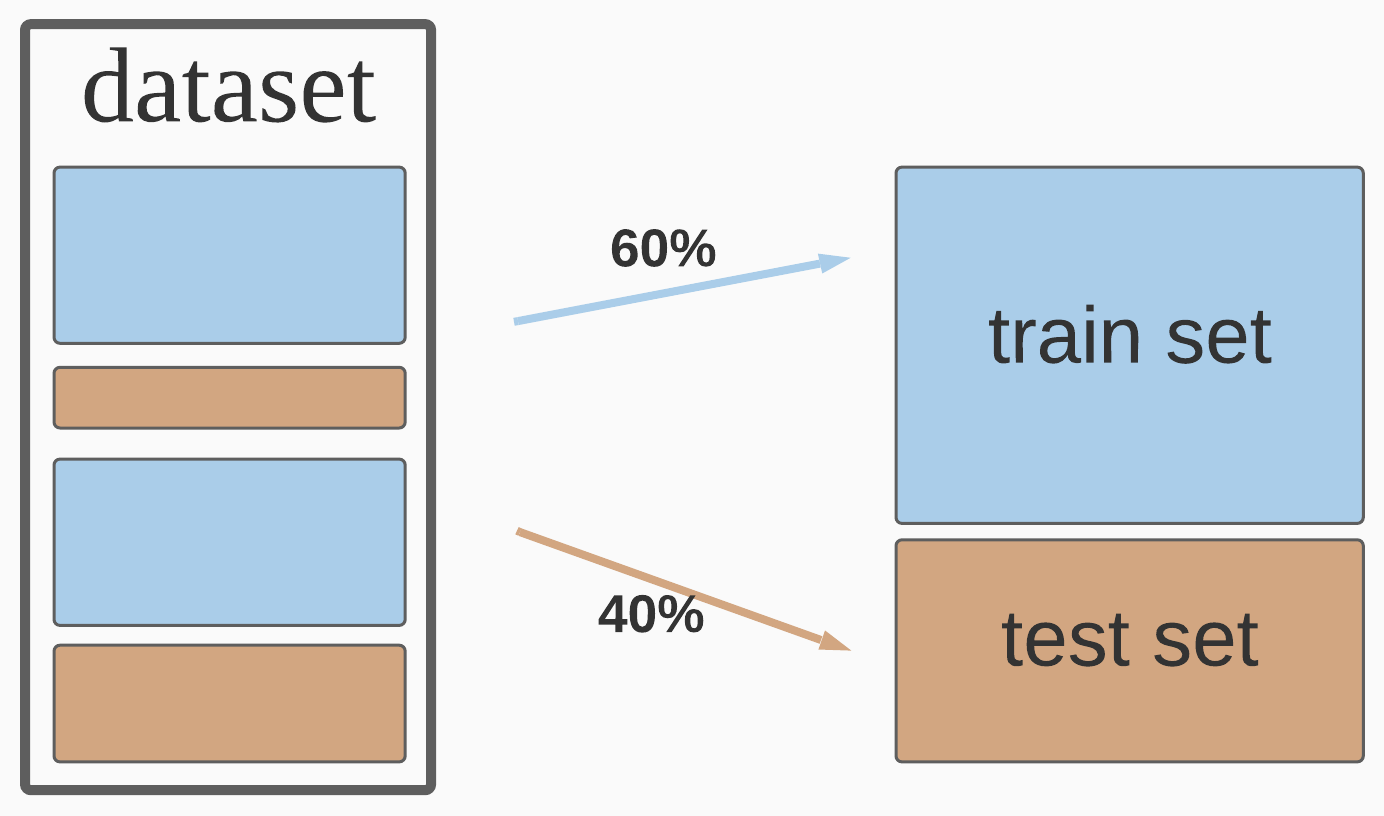
\includegraphics[width=.6\textwidth]{figures/chap3/ml/train_test}
    \caption{Data set split in 2 subsets: a train set and a test set by 60/40 ratio.}
    \label{c3:fig_train_test}
\end{figure}

In cases with extended experiments, the risk to overfit the network's hyperparameters to a certain test set is increased. To prevent the selection of hyperparameters that perform well only on the selected test set, we create a third subset, the \textit{validation set} $X_{val}$. 
A common practice to acquire a validation set is to split the existing training set or in case where access to large sets of data in not the case validation can have the same ration as the test set.
In practice, the network is trained as usual and the validation set is used in order to tune hyperparameters and set the model's weights. 
The final model is evaluated on the test set (Figure~\ref{c3:fig_train_val_test}).

\begin{figure}[h!]
    \centering  
    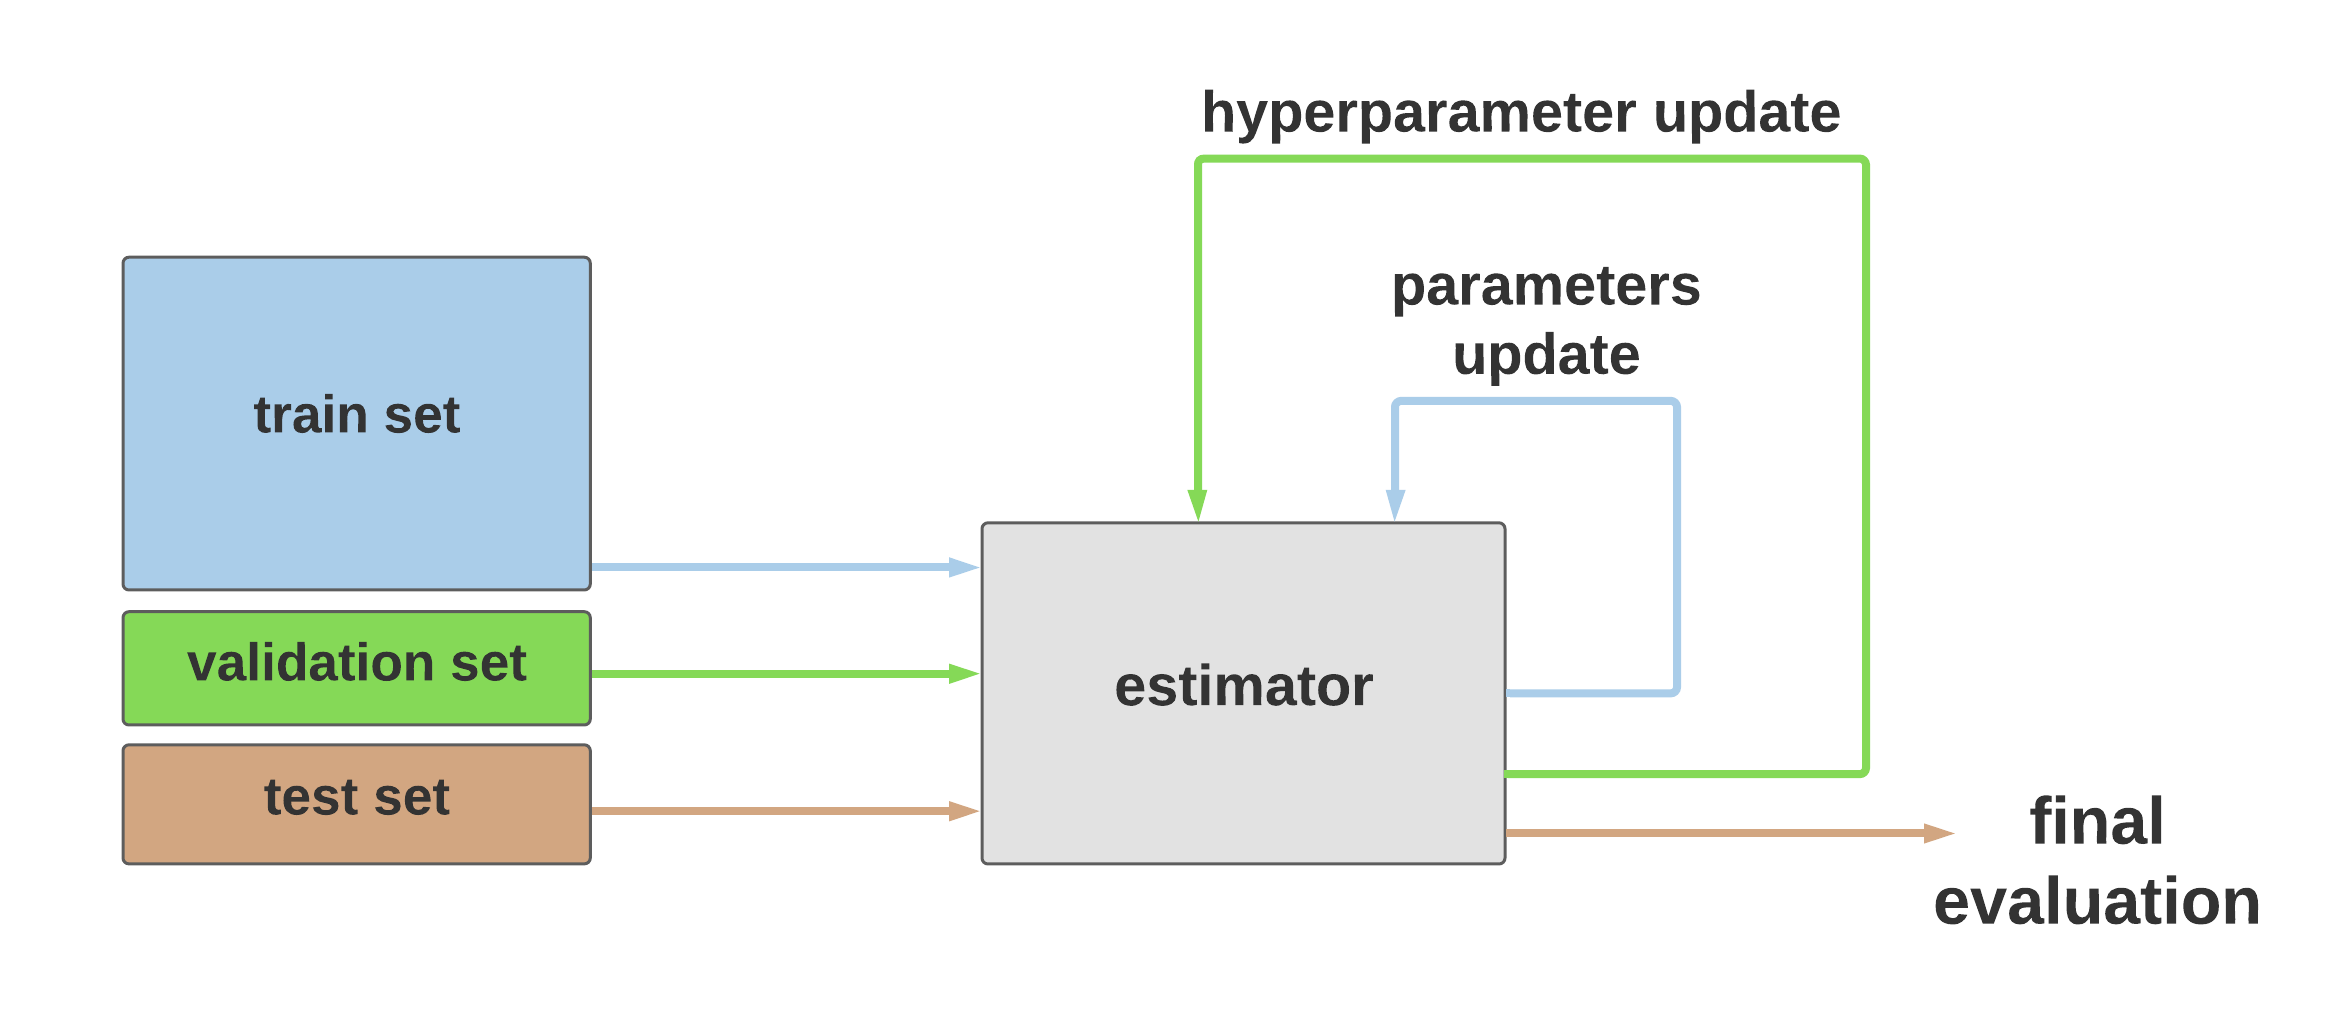
\includegraphics[width=.8\textwidth]{figures/chap3/ml/train_valid_test}
    \caption{Training process of an estimator. Train set is used to update model's parameters(weight and biases). Validation set is used to tune model's optimal hyperparameters. Test set is used for the objective performance evaluation of the classifier.}
    \label{c3:fig_train_val_test}
\end{figure}


\section{Regularization}

Training a deep neural network is considered an art rather than a typical procedure. The choice of hyperparameter is not limited in the number of layers, convolution filter size etc.  but is expanded to the subtle selection of other hyperparameters. Some of them are weight initialization techniques, learning rate decay, early stopping, dropout and batch normalization layers.

In this section we will discuss about dropout and batch normalization since the rest of techniques are briefly presented in Section~\ref{c5:section_passive_learning}.

\textbf{Dropout}~\cite{srivastava2014dropout} is one of the oldest regularization techniques in deep learning, Figure~\ref{c3:fig_dropout}. At each training iteration, it drops random neurons from the network with a probability p (typically 25\% to 50\%). In practice, neuron outputs are set to 0. The net result is that these neurons will not participate in the loss computation this time around and they will not get weight updates. Different neurons will be dropped at each training iteration.

\begin{figure}[h!]
    \centering  
    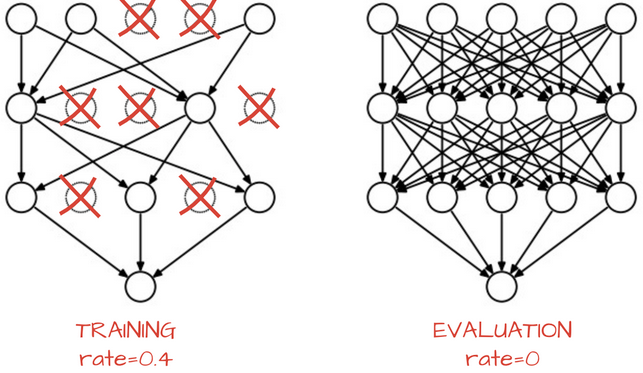
\includegraphics[width=.7\textwidth]{figures/chap3/ml/dropout}
    \caption{Dropout demonstration during training with 40\% neuron drop. In evalution(inference) all the neuron are used.}
    \label{c3:fig_dropout}
\end{figure}

A more complex technique called \textbf{batch normalization} tries to address a problem, known as \textit{internal covariate shift}~\cite{ioffe2015batch}, which relates to how neuron outputs are distributed relatively to the neuron's activation function by the time. 
At the beginning, network parameters are randomly initialized while during training these parameters are varying. The variations in the distribution of neuron's activations has a property to ``confuse'' the next layer and so forth to destabilize the training.\

In the bottomline, \textit{batch normalization} aims to stabilize the training process by minimizing exploding gradient issues, helps the network to converge and usually allows to decrease the dropout rate, or even acts as a substantial to regularize overfitting.

\section{Convolutional Neural Networks}

Deep neural networks are hierarchical learning systems, in which high-level features are obtained by composing the low-level ones. In images, local combined features of edges form motifs, motifs assemble into parts and parts create objects.
Convolutional neural networks (CNN) are inspired by neuroscience and more specifically the overall architectures mimic the human visual cortex, as we showed in Section~\ref{c2:sec_iaqa}.
Marr~\cite{marr1982vision} claimed that the attributes carrying the valuable information in an image, may emerge at any of a range of scales in the real world.
He formulated a physical assumption on hierarchical organizations of the visual world that in simple terms supports that the human representation mechanism must work under a number of different scales in order to capture changes in \textit{depth} and \textit{surface orientation}.

The above statement is the core function in the design of a CNN. Convolutional networks are designed to process data that come in its raw form, for example a colour image is composed of three 2D arrays containing pixel intensities in RGB colour space. That itself, is a major breakthrough in the domain of pattern recognition, as the use of handcrafted features becames obsolete.

The key ideas behind a CNN can be considered the following:

\begin{itemize}
 \item Automatic feature engineering
 \item Parameter sharing
 \item Local connections
 \item Pooling
 \item Non-linearity
 \item Used in many layers
\end{itemize}

The architecture of a typical CNN in illustrated in Figure~\ref{c3:fig_cnn} and is structured as a series of stages.

The first stages are composed of two types of layers: convolution and pooling layers.

\begin{figure}[h!]
    \centering  
    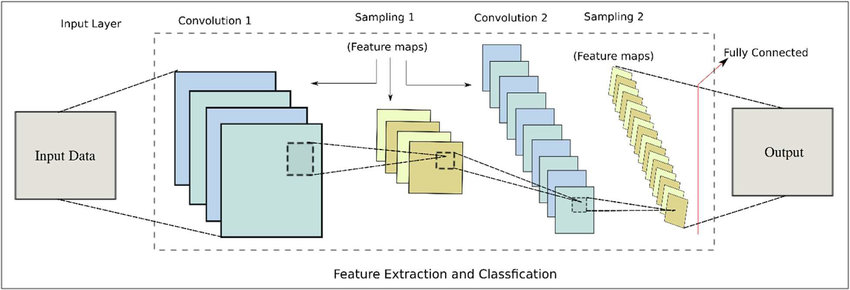
\includegraphics[width=.7\textwidth]{figures/chap3/cnn/cnn_sample}
    \caption{A typical convolution neural network architecture.}
    \label{c3:fig_cnn}
\end{figure}

In a convolution layer, the units are organized in features maps, Figure~\ref{c3:fig_feature_map}, within each unit is connected to local patches in the feature maps of the previous layer through a set of weights(parameter sharing), using a pool of filters. 

\begin{figure}[h!]
    \centering  
    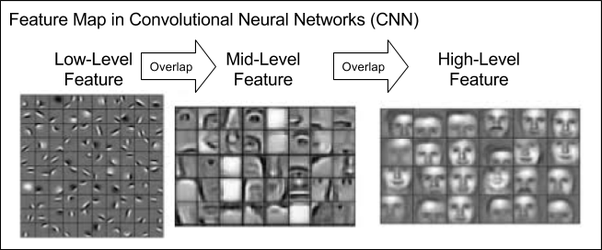
\includegraphics[width=.7\textwidth]{figures/chap3/cnn/feature_map}
    \caption{A hierarchical feature map from low to high level features.}
    \label{c3:fig_feature_map}
\end{figure}

The result of this local weighted sum is then passed through a non-linear function such a ReLU. All units in a feature map share the same filter pool while different feature maps in a layer use different filter pools.

The reason for this technique is twofold.
First, in a image, local groups of values are often highly correlated and form distinctive local motifs that are easily detected.
Second, the local features of images are invariant to translation. More specifically, if a motif may appear in any region of an image, the same pattern can be detected in any region, since units at different locations share the same weights.

However, the role of a convolutional layer is to detect local organizations of features from the previous layers, the role of pooling layer is to merge the semantically similar features into one. A typical pooling layer computes the max or average value of a selected set of output neurons from the convolutional layers and use these as inputs to higher layers.
Because of the relative posititions of the features forming a motif can vary, effective detection can be achieved by downsampling the patch region of each feature, giving the property of invariance to shifts and distortions of the inputs.

After the last concolutional layer, the data is in the form of a ``cube''. In order to pass to the next stage of a CNN, a densely connected layer, there are two ways.

The first one is to flatten the data into a vector and then pass it to the dense layer with a softmax activation.
The second and more cost efficient, is to average all the values and feed these through a softmax activation function. Figure~\ref{c3:fig_flatten_global} illustrates the two methods.

\begin{figure}[h!]
    \centering  
    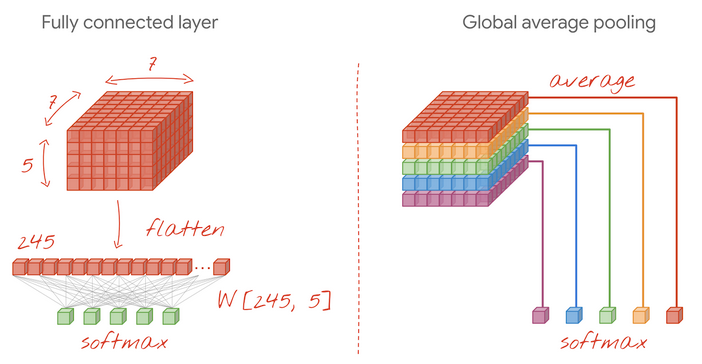
\includegraphics[width=.7\textwidth]{figures/chap3/cnn/flatten_global}
    \caption{Two methods to pass the input of the last convolutional layer to a densely connected layer.}
    \label{c3:fig_flatten_global}
\end{figure}


With these constraints, the model can be quite compact in terms of number of actual parameters. A CNN architecture achieves a substantial reduction in the number of connections concerning to a densely connected network via parameter/weight sharing and pooling layer.

Summing up, a convolutional neural network, is primarly comprised of two levels. The feature extraction level, that is constructed from convolutional and pooling layers, trained to extract better and more robust features. The layer properties allow the use of stacking multiple layers thus forming a deep network structure.
The second level, contain fully connected layers. This layers aim to learn the associations between high-level features of the last convolutional layer with the labels of the input in order to perform classification.

\subsection{Convolution and receptive fields}

In convolutional neural network the key operation is basic linera algebra operation where an a filter or kernel with a set of weights, slides on a input vector. In each slide, an element-wise multiplication between the input and the kernel in performed producing a dot product which is summed, resulting in a single value. Applying a filter to an image will result in a feature map that will have the characteristic of the filter element structure. The operation is visualised in Figure~\ref{c3:fig_convolution}(a). Different type of filters will results in a different feature map(vertical lines, horizontal lines).

By stacking multiple convolutional layers allows a hierarchical decomposition of the input, from low-level features expressed in lines or edges, to high-level features such objects, faces etc.

Pooling is a operation, without dot product level multiplications. Pooling layers does not have weight parameters and perform a simple pooling operation such meam, averaging or max pooling as illustrated in Figure~\ref{c3:fig_convolution}(b).


\begin{figure}[h!]
    \centering  
    \subfigure[]{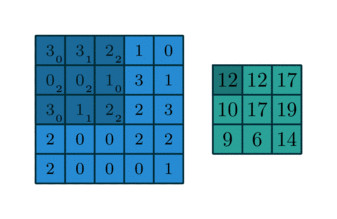
\includegraphics[width=.4\textwidth]{figures/chap3/cnn/conv}}
    \subfigure[]{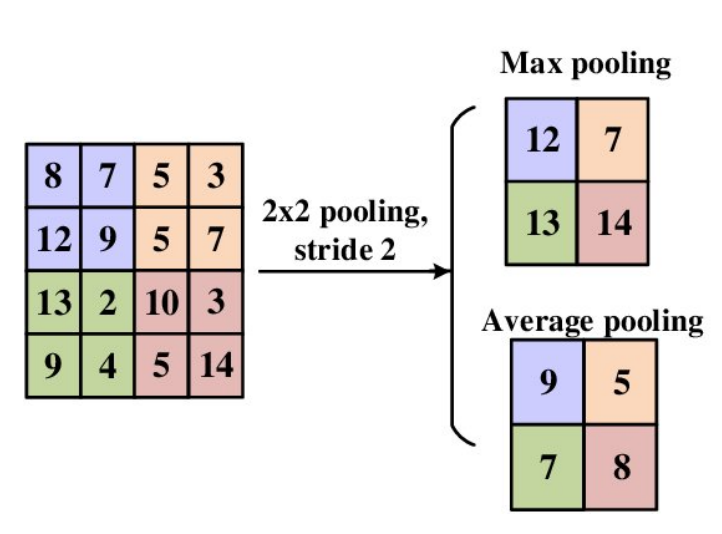
\includegraphics[width=.4\textwidth]{figures/chap3/cnn/pooling}}
    \caption{(a) The operation of convolution between an input(blue) and a kernel(dark-blue) with weights. The out of a single slide is a single number(dark-green). The whole operation produce a new feature map(green). (b) Pooling operation in max and average types of pooling.}
    \label{c3:fig_convolution}
\end{figure}

The notion of a \textit{receptive field} in a deep convolutional architecture is inspired from the human visual system, (Figure~\ref{c3:fig_receptive_field}-a).

In deep learning, the receptive filed is defined as the size of the region in the input that produces the feature~\cite{araujo2019computing}. Receptive field refers only to the feature extraction part of the network, because a convolution unit is connected or depends to only a specific region of the input.
Intuitively, the network's receptive field is the region of an input - not only the input of the network, but any input, can be the output of any network layer - with a relative unit that we consider it as output receiver of the input. For example a simple convolutional operation between a kernel and an input is considered a receptive field. Also the final convolutional layer in respect of the first input layer characterises the total network's receptive field size, (Figure~\ref{c3:fig_receptive_field}-b).

\begin{figure}[h!]
    \centering  
    \subfigure[]{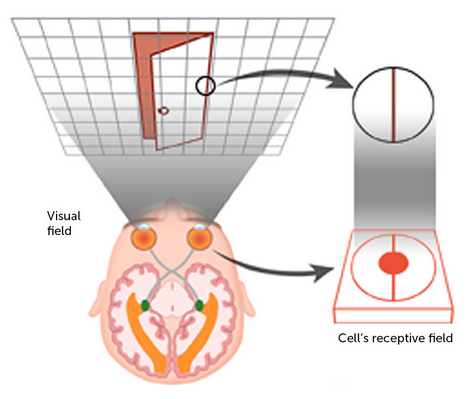
\includegraphics[width=.4\textwidth]{figures/chap3/cnn/human_receptive_field}}
    \subfigure[]{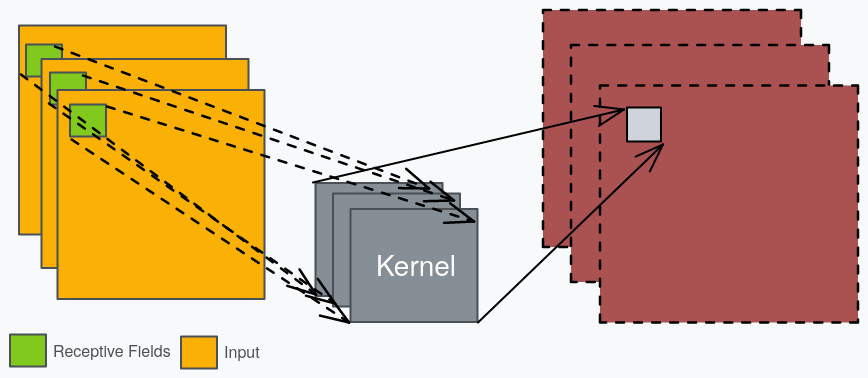
\includegraphics[width=.4\textwidth]{figures/chap3/cnn/receptive_fields}}
    \caption{(a)Human receptive field, (b) Receptive field with convolution operation.}
    \label{c3:fig_receptive_field}
\end{figure}

\section{Deep Learning Architectures}
\label{c3:deep_arch}

In order to increase the receptive field in a convolutional network, there is a variety of ways to achieve it. It can be done by adding more convolutional layers(make the network deeper, add pooling layers, increase convolution striding, use sequential dilated convolutions or add skip connections.
The latter has also regularization properties, because an the network becomes deeper the risk of vanishing gradient problem to appear is higher.

By using a skip connection, we provide an alternative path for the gradient(with backpropagation). At its name suggests, skip connectios, skip some layer in the network and feeds the output of one layer as the input to the next layers~\cite{adaloglou2020skip}.

There are two ways to apply skip connection, with \textbf{addition} and \textbf{concatenation}. In this thesis, we have applied the famous DenseNet~\cite{huang2017densely} architecture which utilises concatenations as skip connections (Figure~\ref{c3:densenet_arch_origin}).

\textit{DenseNet} model starts with a convolutional-pooling block and continues with a series of ``Dense blocks-Transition layer''. Finally it closes with a \textit{Global Average pool} and a \textit{Fully-connected} block.

In every ``Dense block'' the input tensor passes through a series of convolutional operations with fixed number of filters \textit{k} and the result of each one is then concatenated to the original tensor.

Thus the number of feature maps of the input tensor follows an arithmetic growth at every internal stage of the Dense block by \textit{k} tensors per stage.
In order for the size of the tensor to remain manageable the model makes use of the \textit{Transition layers} where the number of feature maps of the input tensor is reduced to half. Also the spatial dimensions of the input tensor are halved by an \textit{Average Pool layer}.

At each \textit{Dense block}, there is a repetition of: (a) $1\times1$ conv with $4\cdot k$ filter, (b) $3\times3$ conv with $k$ filters. Every \textit{Dense block} is constructed by Batch Normalization-ReLU-Convolution sets. The aforementioned modules of DenseNet model are shown in Figure~\ref{c3:densenet_arch_modules}

\begin{figure}[h!]
    \centering  
    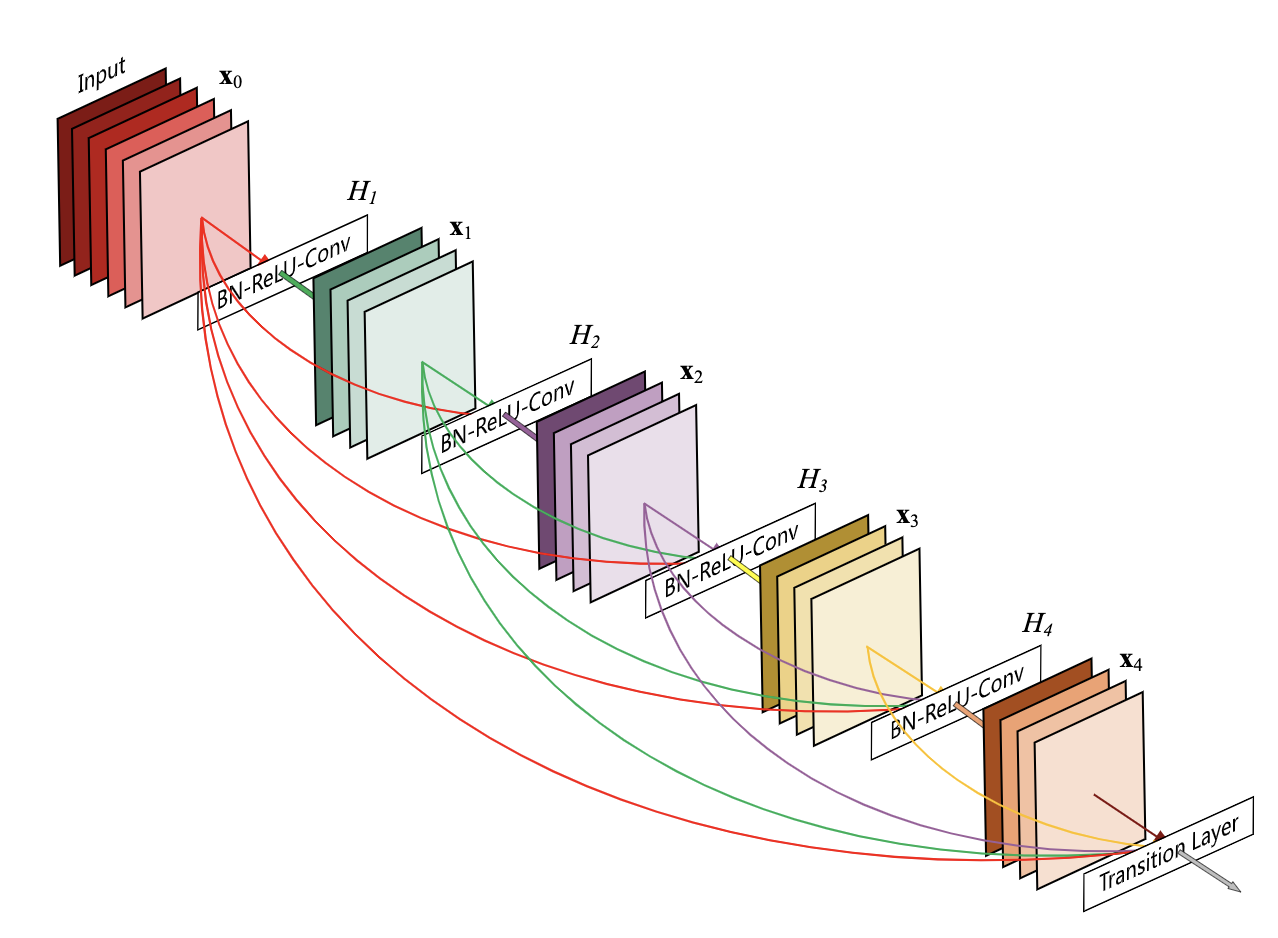
\includegraphics[width=.5\textwidth]{figures/chap3/cnn/architectures/densenet_arch_origin}
    \caption{DenseNet architecture from the original paper~\cite{huang2017densely}}
    \label{c3:densenet_arch_origin}
\end{figure}

\begin{figure}[h!]
    \centering  
    \subfigure[]{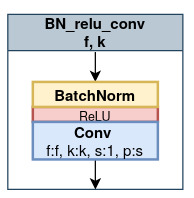
\includegraphics[width=.2\textwidth]{figures/chap3/cnn/architectures/densenet_1}}
    \subfigure[]{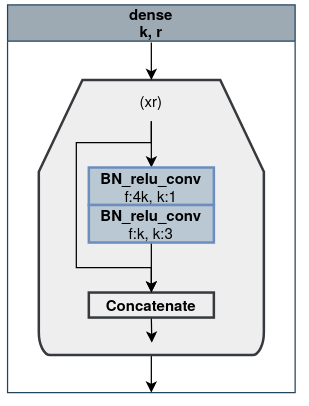
\includegraphics[width=.2\textwidth]{figures/chap3/cnn/architectures/densenet_2}}
    \subfigure[]{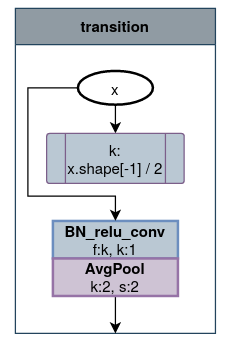
\includegraphics[width=.2\textwidth]{figures/chap3/cnn/architectures/densenet_3}}
    \subfigure[]{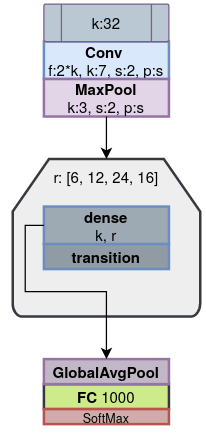
\includegraphics[width=.2\textwidth]{figures/chap3/cnn/architectures/densenet_4}}
    \caption{DenseNet model modules: (a) BN-ReLU-Conv compartment, (b) Dense block, (c) Transition layer, (c) all modules of the original DenseNet}
    \label{c3:densenet_arch_modules}
\end{figure}


More specifically we have implemented a lighter version of DenseNet architecture where more details are presented in Section~\ref{c5:section_passive_learning}, illustrated in Figure~\ref{c3:densenet_arch}.

\begin{figure}[h!]
    \centering  
    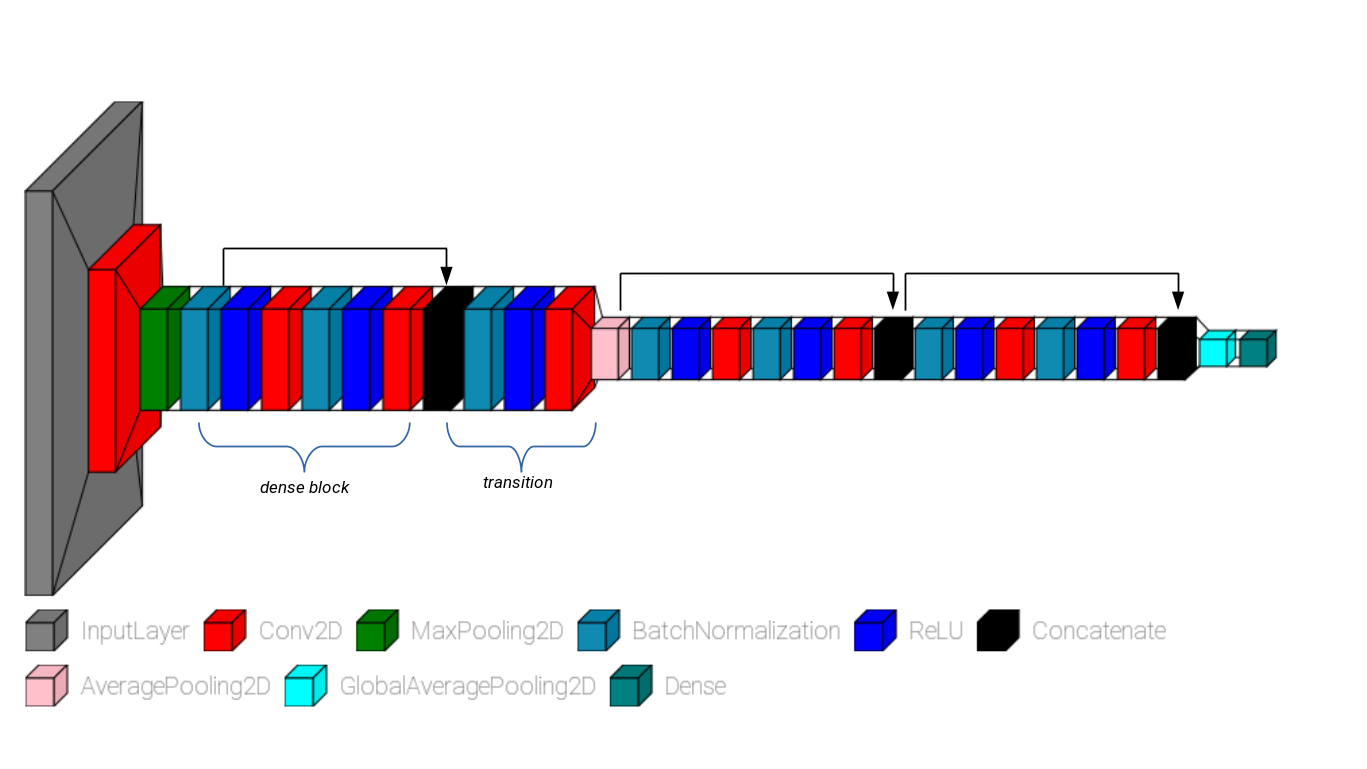
\includegraphics[width=.7\textwidth]{figures/chap3/cnn/architectures/densenet_arch}
    \caption{DenseNet architecture with 1 and 2 consecutive Dense Blocks}
    \label{c3:densenet_arch}
\end{figure}

Another famous architecture, the winner in ImageNet Challenge 2014, is the \textit{VGG16}~\cite{simonyan2014very}. It is a rather simple but very deep architecture of 16 layers. All hidden layers are equipped with ReLU non-linearity and max pooling is performed over a $2\times2$ window, with stride 2.
The network consists of 5 convolutional blocks and 3 fully connected layers. Each convolutional block consists of 2 or more convolutional layers and a max pool layer. 
In this thesis we utilised VGG16 with pretrained imagenet weights while we substitute the last decision layer with globar average pooling, a batch norm layer and a two-output softmax layer.
Figure~\ref{c3:vgg_arch} illustrates the network architecture.

\begin{figure}[h!]
    \centering  
    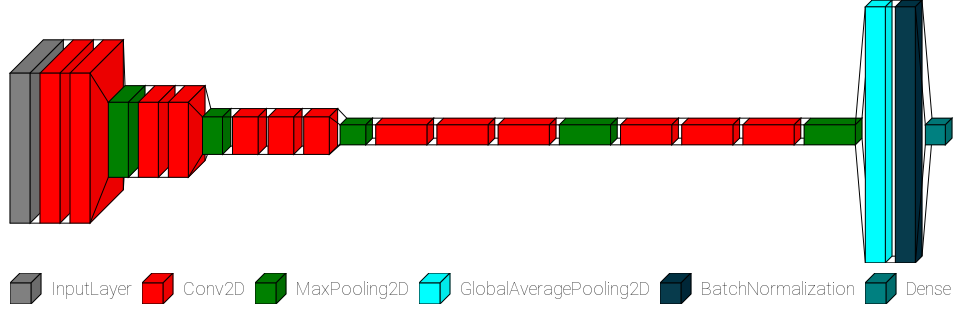
\includegraphics[width=.7\textwidth]{figures/chap3/cnn/architectures/vgg_arch}
    \caption{VGG16 architecture with Global Average Pooling 2D and Batch Normalization layers at the end}
    \label{c3:vgg_arch}
\end{figure}

Moreover, we have created a SimpleNet architecture, inspired from the aforementioned models. We have combined the notion of Dense blocks in DenseNet with the deep layer architecture of VGG16. The network consists of 3 convolutional block and 2 fully connected layers. Each convolutional block consists of 2 or more convolutional layers and a max pool layer. The first layer is consisted of one Dense block, while the rest of two Dense block. After the last convolutional layer a global average pooling layer forwards the input to a fully connected layer, passed to a Dropout, to a softmax decision output.
Figure~\ref{c3:simplenet_arch} depicts the network architecture.

\begin{figure}[h!]
    \centering  
    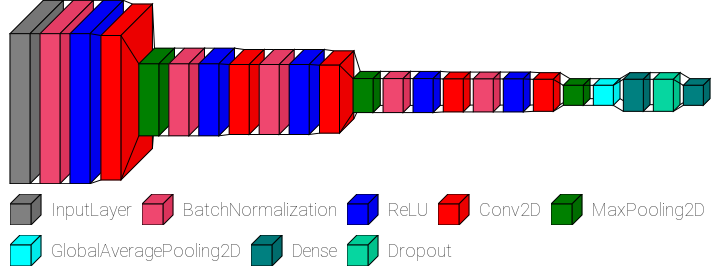
\includegraphics[width=.7\textwidth]{figures/chap3/cnn/architectures/simplenet_arch}
    \caption{A SimpleNet architecture}
    \label{c3:simplenet_arch}
\end{figure}

More details of the network can be found in Section~\ref{c5:section_passive_learning} and in Appendix.

%%%%%%%%%%%%%%%%%%%%%%%%%%%%%%%%%%%%%%%%%%%%%%

\section{Image Aesthetics with Deep Learning}
\label{c3:section_aesthetics_deep}
Image aesthetics quantification is a task that has gained tremendous growth with the use of deep learning techniques from 2014 and later. The research community has adopted the term Image Aesthetics Quality Assessment (IAQA)~\cite{yang2019comprehensive} to approach the problem, which can be divided in five different aesthetic tasks including aesthetic classification, regression, distribution aesthetic factors and description.

Deep learning, like to many other applications, offers and automatic and universal solution to extract features and consequently learn a feature extractor solely based on the input data. In contrast with traditional hand-made feature extractors that require substantial amount of engineering skills and domain expertise, a deep learning approach does not require to master complicated and demanding knowledge.

Major developments in the domain such as the dramatic improvement in the ImageNet classification benchmark from Krizhevsky et al~\cite{krizhevsky2012imagenet} using a DCNN, and the release of the \textit{Analysis of Visual Aesthetics}(AVA) data set in the same year from Murray et al~\cite{murray2012ava}, which contains over 250,000 photos from \textit{DPChallenge.com}, put IAQA again in the spotlight.

Summarizing the recent literature concerning aesthetic classification and regression related tasks in 2014, Lu et al~\cite{lu2014rapid}, proposed RAPID(RAting PIctorial aesthetics with Deep learning) system which adopts a double-column DCNN which combines heterogenous inputs from global and local view of an image to create a unified classifier using AVA dataset.

In 2016, Kong et al~\cite{kong2016photo} assembled a new aesthetics and attributes database (AADB) which contains aesthetics scores in form of star-rating and meaningful attributes mapped to each image given by multiple human annotators. In addition they have proposed a new CNN architecture that unifies aesthetics attributes and photo content for image aesthetic ratings upon a classification problem benchmarking their published data set versus AVA.
Their published data set were collected in co-operation with professional photographers and is closely related to image aesthetic judgements such content, object emphasis, light, colour harmony, vivid colour, shallow depth of field, motion blur, rule of thirds, balanced elements, repetition and symmetry.


Another approach that focus on preserving the image composition fed to a CNN, without damaging the input image by a geometric transformation is proposed by Mai~\cite{mai2016composition}, 2016. Multi-Net Adaptive Spatial Pooling ConvNet(MNA-net) is a compotition-preserving architecture which learns aesthetics features from images retaining their original aspect ratio without any transformation achieved by an adaptive spatial pooling layer on regular convolutional layers placed in network's input. It also allows multi-scale feature extraction achieved from multiple sub-networks with different adaptive spatial pooling sizes, also utilising AVA data set.


A work in 2017 from Malu et al~\cite{malu2017learning} similar to Kong's, attempts to interpret image quality attributes contributing to an overall aesthetic score. They propose a multi-task dcnn which simultaneously learn eight aesthetic attributes the same as above, composition balance, content, colour, depth of field, light, object emphasis, rule of thirds and vivid colours, along with the overall aesthetic score Figure~\ref{c3:aadb}. The have also developed a visualization of feature map activations based on the attributes above to highlight the key regions that correspond to the related feature attribute using the AADB database.

A recent study attempts to solve the same problem by training a dcnn to recognize if an image is appealing or not. Bhandari et al~\cite{bhandari2020image} incorporate a technique that extracts low-level features such colour properties and high level features in order to recognize prominent structures and entities in an image such, salient objects, rule of thirds, depth of field and other. They have created a diversely collected data set from Google, Flickr, Kaggle and at the same time utilize the GrabCut algorithm to efficiently extract the foreground object from a complex environment.

However, inspecting the data sets used in the aforementioned papers, the distinction between ``high'' and ``low'' quality images is more of a stylistic difference than anything else. Figure~\ref{c3:crap} shows a sample from AADB dataset and there is a profound evident of the content quality. Also, Figure~\ref{c3:ava_crap}, shows the image aesthetic classification from the RAPID system.
We would argue, that this style of photography is not by any means close to a known form of art. One can observe, datetime captions, poor sharpness, flat and overwhelming shots from compact cameras or even mobile devices.
Photography is a form of art that adopts the aspect of the visual world and extends it, in the undefined rules of a form that a photographer chooses to transform into a new medium of communication.

\begin{figure}[ht!]
    \centering  
    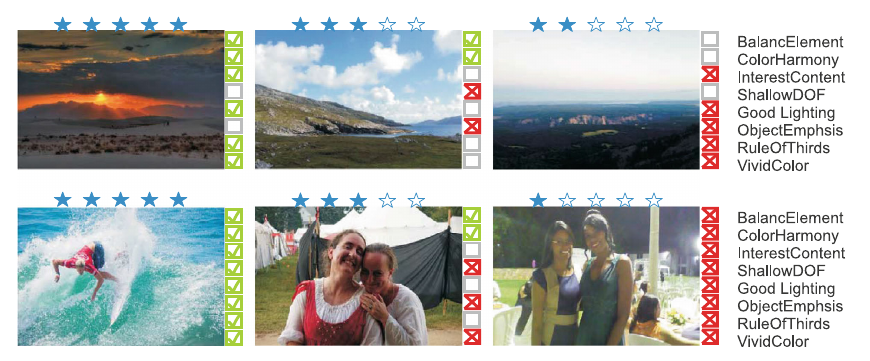
\includegraphics[width=.6\textwidth]{figures/chap2/aesthetics/aadb_dataset}
    \caption{Sample images in AADB dataset. Each photo is annotated with 8 aesthetic attributes in binary labels and aesthetic ratings.}
    \label{c3:aadb}
\end{figure}

\begin{figure}[ht!]
    \centering  
    \subfigure{{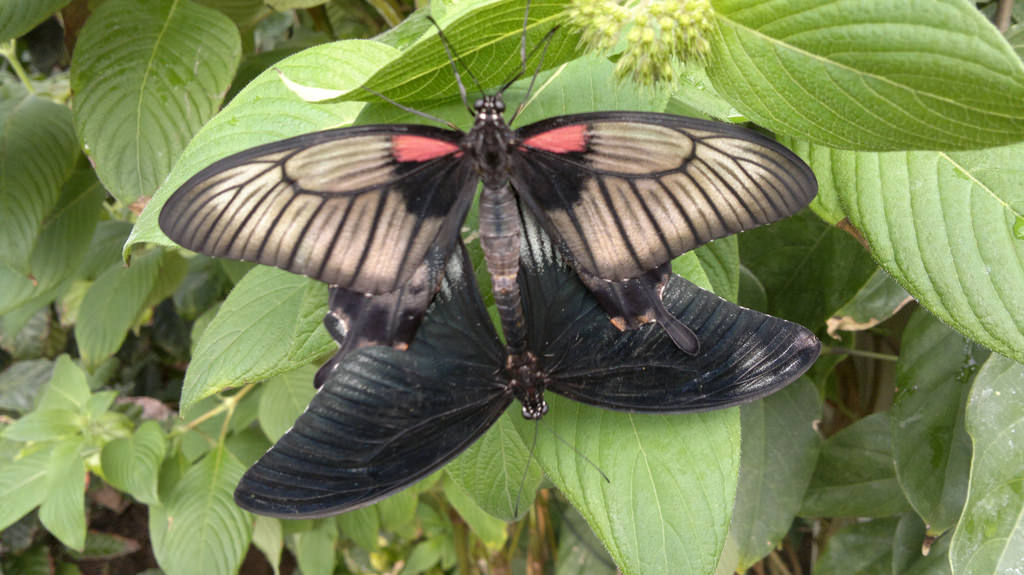
\includegraphics[width=.2\textwidth]{figures/chap3/crap/1}}}
    \subfigure{{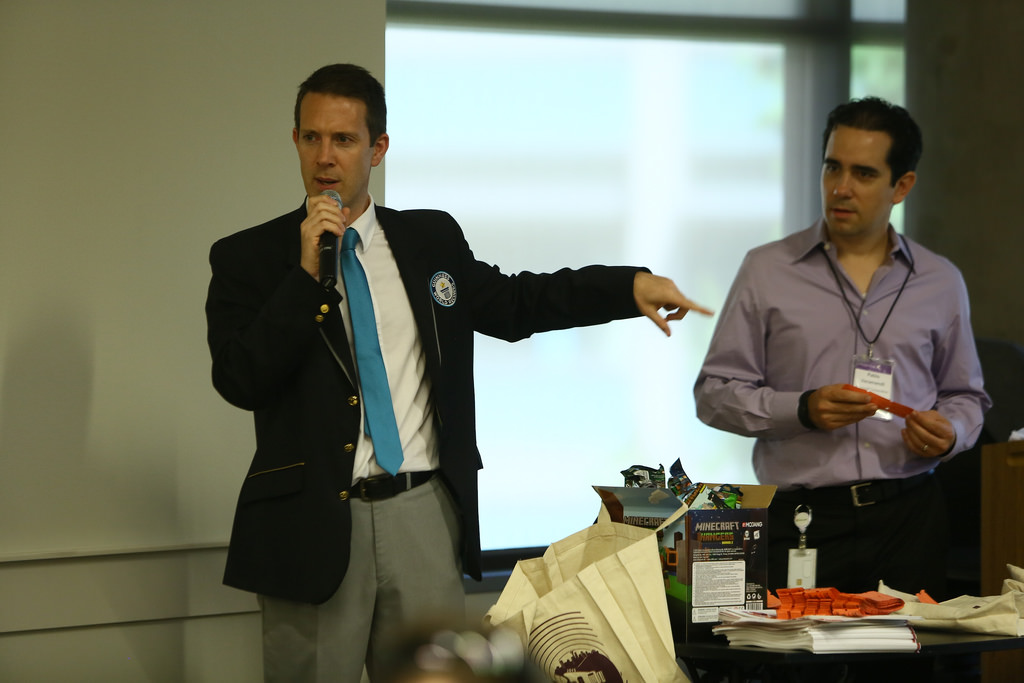
\includegraphics[width=.2\textwidth]{figures/chap3/crap/2}}}
    \subfigure{{\includegraphics[width=.2\textwidth]{figures/chap3/crap/3}}}
    \subfigure{{\includegraphics[width=.2\textwidth]{figures/chap3/crap/4}}}
    \subfigure{{\includegraphics[width=.2\textwidth]{figures/chap3/crap/5}}}
    \subfigure{{\includegraphics[width=.2\textwidth]{figures/chap3/crap/6}}}
    \subfigure{{\includegraphics[width=.2\textwidth]{figures/chap3/crap/7}}}
    \subfigure{{\includegraphics[width=.2\textwidth]{figures/chap3/crap/8}}}
    \caption{Sample figures from AADB dataset}
    \label{c3:crap}
\end{figure}

\begin{figure}[ht!]
    \centering  
    \subfigure[Images ranked the highest in aesthetics by DCNN]{{\includegraphics[width=.5\textwidth]{figures/chap3/crap/ava_good}}}
    \subfigure[Images ranked the lowest in aesthetics by DCNN]{{\includegraphics[width=.5\textwidth]{figures/chap3/crap/ava_crap}}}
    \caption{RAPID system, Lu et al. 2014~\cite{lu2014rapid}}
    \label{c3:ava_crap}
\end{figure}    
    
In the next Chapter, we present a recently published high competent data set, with super high resolution images, from Unsplash, a famous image sharing and publishing platform, adopted by famous products and web applications across industry.


%%%%%%%%%%%%%%%%%%%%%%%%%%%%%%%%%%%%%%%%%

\section{Active Learning}

In the latest decade, deep learning models have achieved groundbreaking results on several computer vision tasks~\cite{he2015delving},~\cite{krizhevsky2012imagenet},~\cite{he2016deep} and have become very popular due to their high flexibility, capacity and accuracy. Yet these models rely on vast amounts of labelled data for training. In practice, in many applications, we might not have access to such large data pools and more specifically we cannot afford to annotate all of them. Data labelling is an expensive and tedious task that is performed under a limited time budget, in addition the acquisition of a large number of high-quality annotated samples consumes a lot of manpower, making it unfeasible in fields that require high levels of expertise.

However, if there was an algorithm, that had the ability to suggest the samples from which it learns, it would achieve greater accuracy with less annotations.

%What will happen if we keep the model's hyperparameters and architecture fixed and experiment on different versions of data?

The paradigm of choosing the most informative data to label is referred to as \textit{active learning}~\cite{cohn1996active},~\cite{settles2009active}. The key challenge remains that there isn't any standardized method to determine the informativeness of the data. Active learning is performed in the context of sequential decision making where at every step, two operations are performed: i) measure the informativeness of the unlabelled data w.r.t. an active learner and choose the most informative to annotate, ii) update the underlying training data set with the new annotations and the active learner w.r.t. to the training performance.

Active learning is a training strategy, that aims to select the most beneficial samples from the unlabelled data set and send them to the oracle(human annotator) for labelling, in order to reduce the cost of labelling as much as possible while achieving high performance.

There are several \textit{scenarios} which an active learner can utilise and pose queries and several \textit{query strategies} that can been used to decide which instances are most informative.

\subsection{Active learning scenarios}

In random selection or in regular ``passive'' learning, the process is straightforward and new samples are chosen to get labelled uniformly from an unlabelled pool.

When employing an active learning scenario, we ask the active learner from a pool of unlabelled instances, to indicate the most informative samples that when included in training set will be more beneficial and perform better, in less training rounds, comparing to when trained with randomly selected samples.

Such active learning scenarios are considered the i) \textbf{Membership query synthesis}, ii)\textbf{Stream-based selective sampling} and iii) \textbf{Pool-based active learning}~\cite{settles2009active}, but only some of them can apply to our case study.

Membership query synthesis means that the learner can request to query the label of any unlabelled sample in the input space while in stream-based sampling, an independent judgement is made from the learner, on whether each sample in the data set is considered for annotation. The latter is rather the most expensive comparing to other methods as an additional mechanism is needed for the learner to decide if the candidate sample belong to the underlying distribution.

In pool-based scenario, unlabelled instances are selectively drawn from the pool and are typically queried in a greedy fashion, according to an informativeness measure used to evaluate all instances in the pool.

Applying the first scenario to our case study when querying from the pool of unlabelled instances the unexpected problem we encountered is that many of the query images generated were not contain any semantic meaning about the certain photography style (shallow/deep depth of field). 

Pool-based seems that applies better to our case study and based on an informativeness measure we can generate actively selected samples. In order to tackle the encountered problem, inspired from the second scenario, during the process of annotation, the problematic candidate samples where discarded from the selection. Finally we constructed a closed data set pool in order to apply the pool-based scenario.

Figure~\ref{c3:fig_pool_based} illustrates the framework diagram from pool based strategy. To initialise the process(bootstrap), we can select randomly samples from unlabelled pool \textit{U}, obtain labels in order to generate a labelled training set \textit{L} and train a machine learning model \textit{C}. Next, we use this model as an active learner, by applying a query strategy framework in order to select the next annotated samples. The process is repeated until the label budget is exhausted or the termination conditions are met(e.g. data depletion, query strategy limits).

\begin{figure}[ht!]
    \centering  
    {\includegraphics[width=.5\textwidth]{figures/chap3/active_learning/pool_based}}
    \caption{Pool based active learning}
    \label{c3:fig_pool_based}
\end{figure} 

\subsection{Query strategy framework}

The simplest and most commonly used query framework is uncertainty sampling, where an active learner queries the samples that it can predict with least confidence (LC)~\cite{settles2009active}. Those samples are considered as the most informative ones or the most ambiguous, as the classifier is uncertain for the predicted class. This of course requires the use of a model that is capable of assessing adequately the prediction uncertainty.

The aforementioned query strategy when applied in DAL can be implemented with the output of the softmax layer of the deep learned classifier, thus the query strategy based on uncertainty is widely used in a variety of studies~\cite{ren2020survey}.

For this reason, Deep Bayesian Active Learning (DBAL)~\cite{gal2017deep} has been developed. For a given input set $\text{X}$ and the network output $\text{Y}$ belonging to class, the probabilistic neural network can be defined as $f(x;\theta), p(\theta)$ is a prior on the parameter space $\theta$, and the likelihood $p(y = c|x,\theta)$ is usually determined by $\text{softmax}(f(x;\theta))$. The goal is to obtain a posterior distribution over $\theta$, as follows:

\begin{ceqn}
\begin{align}
    p(\theta|X,Y) = \frac{p(Y|X, \theta)p(\theta)}{p(Y|X)}
\end{align}  
\end{ceqn}

For a new given(inferenced) observation $x^*$, a $\hat{y}$ prediction is made:

\begin{ceqn}
\begin{align}
    p(\hat{y}|x^*, X, Y) = \int p(\hat{y}|x,\theta) p(\theta|X, Y)d\theta
\end{align}  
\end{ceqn}

Thus, least confidence(LC) measurement is given from:

\begin{ceqn}
\begin{align}
     x_{LC}^{*} = argmin_{x} P( \hat{y} | x;\theta ) 
\end{align}  
\end{ceqn}

where $\hat{y} = \text{argmax}_y P(\hat{y}|x;\theta)$, is the most likely predicted class. 

Hence, we use the probabilities as indicators of classification uncertainty.


\subsection{Batch-Mode Deep Active learning}
\label{c5:section_batch_mode_learning}
Formulating the above, we are looking for these samples that will be selected from the active learner, transferred systematically to a human annotator(oracle) and consequently will returned back to the training set, get the model retrained and so forth, achieve better classification performance.

In most active learning research, queries are selected in serial, e.g. one at a time. For the context of DL, the one-by-one sample query method which commonly used in AL is not applicable.
Consider also that sometimes a distributed, parallel labelling environment may be available, e.g. labels are obtained from multiple annotators at the same time.

Selecting queries in serial may be inefficient and in contrast, \textit{batch-mode} active learning allows the learner to query instances in batches which resembles a parallel labelling practice or models with slow training procedures~\cite{settles2009active}.


Moreover, many ML algorithms don't re-train sequentially or retraining does not provide a statistically significant impact on the model, as is the case for many DL models.
In addition, this query method is not only inefficient in the training of the DL model, but can also easily lead to overfit~\cite{zhdanov2019diverse}.

Although there is not any standard rule to determine the number of batches that can be used to an active learning experiment there are works that compare and assess multiple volumes of active batches~\cite{gissin2019discriminative}. In this thesis we choose to experiment in two options. One with variable size of batch without incremental training and an option with a standard batch size of 100 samples and incremental training.


\subsection{Deep Active Learning}

DL has demonstrated abilities to process high-dimensional data though the automated feature extraction mechanisms, while AL has substantial potential to reduce annotation costs. Therefore, combining the two approaches, will effectively benefit the applications performance.

Recent studies and developments in Deep and Active learning are transitioning from the model-centric to the emerging field of data-centric artificial intelligence~\cite{bosser2020model},~\cite{motamedi2021datacentric} which is expected to deliver techniques for data set optimization, thereby to more efficient training with less samples and annotations. 

This falls into an active learning framework with deep learning, known as deep active learning (DAL), that will be able to select the most informative samples, send them to an oracle for annotation and append them to the data set, as it is shown in Figure~\ref{c4:fig_al_procedure}.

\begin{figure}[ht!]
    \centering  
    \includegraphics[width=\textwidth]{figures/chap5/al/al_map}
    \caption{A typical example of DAL: A DL model is pre-trained on the labelled training set \textit{$L_0$}, and given a query strategy is used to select the next samples from the Unlabelled pool \textit{U}. A sampling strategy is to pick the candidate images and they are sent to a human oracle for annotation. The new labelled training set \textit{L} updates the initial \textit{$L_0$} and retrains the Deep Learning model.}
    \label{c4:fig_al_procedure}
\end{figure}

However, we have to consider two things. Deep learning poses several difficulties when used in an active learning setting. First, we have to be able to handle small amounts of data, yet recent developments in deep learning require large amounts of data~\cite{krizhevsky2009learning},~\cite{krizhevsky2012imagenet}. Second, many AL strategies rely on prediction uncertainty and such a case is rare in deep learning~\cite{gal2017deep}.
Concerning the latter, there are studies~\cite{wang2014new},~\cite{wang2016cost} that pose an unreliability to softmax when used to estimate the informativeness of the unlabelled samples and argue that the results may be worse than random selection.

In this thesis, we are studying a challenging and non trivial task thus we will follow the simplest approach using DBAL to exploit an active learning indicator and consequently implement and active learning algorithm.

Active learning using deep learning aims to achieve the best learning result given a limited labelled data set. Given a budget on the available unlabelled instances to have them annotated, our objective is to maximize the classifier's performance with the less cost effective method.

At each iteration, an active learning algorithm has two stages: a) identify a set of unlabelled instances and send them to a human oracle for annotation; and b) train a classifier using both the new and the previously labelled instances. The second stage (train the classifier) can be done in a fully or weakly-supervised manner. 
Fully-supervised is the case when the classifier is trained using only human labelled instances. Weakly-supervised is the case where training runtime utilise the points which are not labelled yet. Although the existing literature focuses most on the active learning for fully-supervised models, we consider both cases in our experiments.


\subsection{Cost Effective Active Learning (CEAL)}
\label{c5:section_ceal}

Another technique different from the existing AL approaches that consider only the most informative samples to get labelled from a human annotator, is one that poses the most confident queried unlabelled samples and automatically pseudo-annotates them without active user labelling.
Samples queried to an active learner with high predicted confidence are the most certain to get classified correctly. The method that selects these samples and automatically assign the predicted class as a pseudolabel, with any human labor cost, is proposed as cost-effective active learning (CEAL)~\cite{wang2016cost}. Figure~\ref{c5:figure_ceal} illustrates the method.

\begin{figure}[ht!]
    \centering  
    \includegraphics[width=\textwidth]{figures/chap5/al/ceal}
    \caption{CEAL progressively feeds the samples from the unlabelled data set into the CNN. The clearly classified samples are pseudolabelled while the most uncertain are send to manual annotation.}
    \label{c5:figure_ceal}
\end{figure}


\subsection{Cached Annotation Batch-Mode Active learning}
\label{c5:section_cached_setting}

Following a closed loop strategy, similar to the Figure~\ref{c4:fig_al_procedure}, it requires the model to be retrained on the whole labelled data set, once new labels are available. For very large modern deep CNN's that require many hours of end-to-end training, this is typically impractical.

% prepei na koitame kai thn pragmatistiki plevra toy provlimatos kai oxi mono tin ideati
In practice, this scenario is often unrealistic: in order to be able to implement such a loop in a production environment the budget for human annotations is limited or might be a deterring factor to construct a fully automated pipeline.
Also the AL strategy has to be closely integrated with the annotation system, something that may introduce limits to the data owner.

In this work, inspired from pool based and batch-mode strategies, we have combined and evaluated both methods in two different active learning settings, that we present in Section~\ref{c5:section_experimental_setup}.

The intuition behind both settings is that they do not adhere in a closed training-query-annotation loop, thus do not require to ask or wait for new labels. All queried ``unlabelled'' samples have been annotated once (pre-annotated) given a time budget. This practice enables the machine learning practitioner to construct a fully automated pipeline without waiting for unlabelled samples to get labelled, instead the active learning algorithm can be designed on what samples will pick next.

We create a new setting of ``caching'' the annotations and named it after ``Cached Annotation Batch-Mode Active Learning''. 
A closed sampling pool is comprised from randomly and actively selected samples, with ``cached'' annotations obtained once at the bootstrap step.

More specifically in Section~\ref{c5:section_al_simulation} we apply a simulation algorithm with \textbf{single} and \textbf{increamentally} trained active learners, on the same pool of pre-annotated samples and demonstrate random and active selection strategies, without asking for extra annotations.

\newpage

% -------------------- Chapter 4 --------------------------------------- #
\chapter{Data Description} \label{c4:intro}
\epigraph{\itshape ``To me, photography is the simultaneous recognition, in a fraction of a second, of the significance of an event.''}
{---Henri Cartier-Bresson}

\section{Unsplash Dataset}

% eda
% image preprocessing
% exif based annotation
% dof based annotation

Unsplash dataset is a publicly available collection of super high resolution photos.~\footnote{https://unsplash.com/data} 

In Section~\ref{c4:image_preprocessing} we describe the image preprocessing methodology we implemented to reformat the dataset's images into a unified format.
Section~\ref{c4:eda} presents an exploratory data analysis, performed to provide a general knowledge base for our case study.
Section~\ref{c4:binning} elaborates on binning process, based on EXIF metadata used as features.
Section~\ref{c4:exif_dataset} covers the methodology we followed to construct a new labelled data set, the \textit{EXIF} data set, based on EXIF metadata characterizing photographs with a photography style.
In Section~\ref{c4:problem_formulation} we come up with the problem formulation, derived from the aforementioned methodologies. The distribution of photography style characteristics that are reflected in Unsplash data set, played a very important role to acquire a solid understanding for its photography aspect.
In Section~\ref{c4:dof_dataset} we present a second data set, the \textit{DoF} data set, annotated with completely manual method based solely on qualitative characteristics of the images.


\section{Image Preprocessing}
\label{c4:image_preprocessing}

Aside from data preprocessing in supplementary data which will be handled as labels, the trained samples which help up solving the problem are RGB images. Image preparation is an essential process in order to feed a dataset of images in a convolutional network, at the same size.
In the case of EXIF dataset, we have created three individual datasets.
The one with both image orientations will be transformed into square images with zero padded pixels in left and right for a vertical oriented image and up and down for a horizontal image.
For the rest of the dataset, horizontal and vertical, we keep them in the same orientation.

Complementary to resizing we are choosing to keep the original aspect ratio of images. 
For aesthetic reasons changing the ratio will impact where the subject is positioned in relation to the sides of the frame. 
If we just resize a photo to the desirable target size, in many cases the final outcome will be distorted and the subject composition will get altered.
In photography the most usual aspect ratio of a captured photo is $3/2$. It has not been established by chance, as it is based on the golden ratio of Fibonacci spiral~\ref{c4:golden_ratio} and has thoroughly adopted by the most famous photographers~\ref{c4:golden_photographer}.

\begin{figure}[ht!]
    \centering  
    \includegraphics[width=.3\textwidth]{figures/chap4/figures/golden_ratio}
    \caption{The golden ratio}
    \label{c4:golden_ratio}
\end{figure}


\begin{figure}[ht!]
    \centering  
    \subfigure{\includegraphics[width=.45\textwidth]{figures/chap4/figures/golden_adams}}
    \subfigure{\includegraphics[width=.45\textwidth]{figures/chap4/figures/golden_brenson}}   
    \caption{Left: Ansel Adams, Right: Henri Cartier-Bresson}
    \label{c4:golden_photographer}
\end{figure}

The target image size for horizontal images is equal to (300,200) for horizontal images,equal to (200,300) for vertical images and equal to (400,400) for datasets with both orientations.
During image resize, \textit{inter area interpolation} were applied, to resample using pixel area relation. This technique offers moire-free results, a geometrical pattern produced in various digital imaging and computer graphics techniques due to undersampling.
To preserve the aspect ratio we have calculated the ratio of the target axis to the maximum reference image axis resolution. 
For an image that its original size is above or bellow the target ratio ($3/2$), the final outcome after the resize, will be a larger image which needs to get cropped or a smaller image which need to get padded with zeros.
The aforementioned transformation process is described in Algorithm~\ref{c4:algorithm}. Additionally, we have provided a meaning full representations of the transformed images in Figures~\ref{c4:horizontal_crop}-\ref{c4:square_transformation}.

\begin{algorithm}
\caption{Image transformation}
\label{c4:algorithm}
\begin{algorithmic}[1]
\Procedure {Resize\_Image}{$image$, $target.width$, $target.height$, $orientation$}
    \If{orientation == Horizontal}
        \State $ratio \leftarrow target.width/max(image.size) $
    \ElsIf{orientation == Vertical}  
        \State $ratio \leftarrow target.height/max(image.size) $
    \EndIf

    \State $new\_size \leftarrow [image.width*ratio, image.height*ratio]$
    \Comment {calculate new size}

    \State $new\_image \leftarrow resize(image, [new\_size.width, new\_size.height], \text{INTER\_AREA\_IP}) $
    \State
    \If{$new\_image.width \neq target.width$}
        \Comment {crop/pad $\rightarrow$ target width}
        \State $new\_image \leftarrow pad\_crop(new\_image, target.width)$
    \ElsIf{$new\_image.height \neq target.height$}
        \Comment {crop/pad $\rightarrow$ target height}
        \State $new\_image \leftarrow pad\_crop(new\_image, target.height)$
    \EndIf
\EndProcedure
\State
\Procedure {pad\_crop}{$image$, $target.width$}
    \If{image.width $>$ target.width}
        \Comment {Evenly Crop image}
        \State $rows\_to\_crop \leftarrow target.width - image.width$
        \State $split\_rows \leftarrow rows\_to\_crop$ \text{DIV} 2
        \If {rows\_to\_crop MOD 2 == 0}
            \State $new\_image \leftarrow image[width-split\_rows: split\_rows]$
        \Else \Comment {Rows to crop odd number, crop one more}
            \State $new\_image \leftarrow image[width-split\_rows: split\_rows+1]$
        \EndIf
    \Else
        \Comment {Evenly 0Pad image}
        \State $rows\_to\_pad \leftarrow target.width - image.width$
        \State $pad\_rows \leftarrow rows\_to\_pad$ \text{DIV} 2
        \If {rows\_to\_pad MOD 2 == 0}
            \State $new\_image \leftarrow$ PADDING0(image, $pad\_rows$)
        \Else \Comment {Rows to pad odd number, pad one more}
            \State $new\_image \leftarrow$ PADDING0(image, $pad\_rows+1$)
        \EndIf
    \EndIf
\EndProcedure
\end{algorithmic}
\end{algorithm}



\begin{figure}[ht!]
    \centering  
    \subfigure{\includegraphics[width=.30\textwidth]{figures/chap4/photos/preprocessing/horizontal/crop/horizontal_resized_with_ratio}}
    \subfigure{\includegraphics[width=.30\textwidth]{figures/chap4/photos/preprocessing/horizontal/crop/horizontal_resized_with_ratio_crop_y}}
    \subfigure{\includegraphics[width=.30\textwidth]{figures/chap4/photos/preprocessing/horizontal/crop/horizontal_resized_without_ratio}}
    \caption{Horizontal Crop, Left: Resized preserving ratio (325x200), Middle: Resized preserving ratio \& Crop to target (300,200), Right: Resized to target without preserving ratio}
    \label{c4:horizontal_crop}
\end{figure}

\begin{figure}[ht!]
    \centering  
    \subfigure{\includegraphics[width=.30\textwidth]{figures/chap4/photos/preprocessing/horizontal/pad/horizontal_resized_with_ratio}}
    \subfigure{\includegraphics[width=.30\textwidth]{figures/chap4/photos/preprocessing/horizontal/pad/horizontal_resized_with_ratio_pad_y}}
    \subfigure{\includegraphics[width=.30\textwidth]{figures/chap4/photos/preprocessing/horizontal/pad/horizontal_resized_without_ratio}}
    \caption{Horizontal Pad, Left: Resized preserving ratio (300x177), Middle: Resized preserving ratio \& 0Pad to target (300,200), Right: Resized to target without preserving ratio}
    \label{c4:horizontal_pad}
\end{figure}


\begin{figure}[ht!]
    \centering  
    \subfigure{\includegraphics[width=.20\textwidth]{figures/chap4/photos/preprocessing/vertical/crop/vertical_resized_with_ratio}}
    \subfigure{\includegraphics[width=.20\textwidth]{figures/chap4/photos/preprocessing/vertical/crop/vertical_resized_with_ratio_crop_x}}
    \subfigure{\includegraphics[width=.20\textwidth]{figures/chap4/photos/preprocessing/vertical/crop/vertical_resized_without_ratio}}
    \caption{Vertical Crop, Left: Resized preserving ratio (240x300), Middle: Resized preserving ratio \& Crop to target (200,300), Right: Resized to target without preserving ratio}
    \label{c4:vertical_crop}
\end{figure}

\begin{figure}[ht!]
    \centering  
    \subfigure{\includegraphics[width=.20\textwidth]{figures/chap4/photos/preprocessing/vertical/pad/vertical_resized_with_ratio}}
    \subfigure{\includegraphics[width=.20\textwidth]{figures/chap4/photos/preprocessing/vertical/pad/vertical_resized_with_ratio_pad_x}}
    \subfigure{\includegraphics[width=.20\textwidth]{figures/chap4/photos/preprocessing/vertical/pad/vertical_resized_without_ratio}}
    \caption{Vertical Pad, Left: Resized preserving ratio (168x300), Middle: Resized preserving ratio \& 0Pad to target (200,300), Right: Resized to target without preserving ratio}
    \label{c4:vertical_pad}
\end{figure}

\begin{figure}[ht!]
    \centering  
    \subfigure{\includegraphics[width=.3\textwidth]{figures/chap4/photos/preprocessing/square/1}}
    \subfigure{\includegraphics[width=.3\textwidth]{figures/chap4/photos/preprocessing/square/2}}
    \subfigure{\includegraphics[width=.3\textwidth]{figures/chap4/photos/preprocessing/square/3}}
    \caption{Dataset in squarified transformation for both orientations to 400x400 by 0Padding}
    \label{c4:square_transformation}
\end{figure}


\section{Exploratory Data Analysis}
\label{c4:eda}

The first step to approach an unknown and recently published dataset, could be done with an exploratory data analysis (EDA). Its purpose is to perform a critical process to discover patterns, eliminate data anomalies and summarize main dataset's characteristics with the help of graphical representations to uncover certain aspects.

In a first level exploration the goal is to identify and comprehend the supplementary data(metadata) aside from images. We are looking for  identifier columns and levels for a categorical variable. In order to achieve that, we project the list of the available feature columns, perform a data cleansing process and create uni-variate histograms.

The scope beyond first level analysis, is to manually construct a labelled dataset relying solely on EXIF features. By applying a binning strategy based on photography domain knowledge, we aim to create data bins for each of the features in order to assign an appropriate label.
Uni-variate binning will aid us to form an initial hypothesis and setup a dataset driven problem that will be used as an indicator for a specific photography style classification problem.

Complementary to the EXIF-based labelled dataset, using the insights from the EDA, we have manually labelled a dataset based on the qualitative characteristics of a certain photography style.
The aforementioned process is depicted in Figure~\ref{c4:etl}.

\begin{figure}[ht!]
    \centering  
    \includegraphics[width=.9\textwidth]{figures/chap4/etl}
    \caption{ETL process}
    \label{c4:etl}
\end{figure}

\subsection{Data Cleaning}
\label{c4:data_cleaning}

\textbf{Photos} dataset is comprised of \textbf{25318} samples in total with more than 15 features and photography metadata, that only a few can be considered as features or candidate labels.
In our case study, we focus only on EXIF(exchangeable image file format) metadata such \textbf{ISO}, the digital sensor's sensitivity, lens \textbf{aperture} value, lens \textbf{focal length} and shutter's \textbf{exposure time} as they represent the camera settings when a picture is captured. Additionally we have included \textbf{width} and \textbf{height} as they denote the picture's orientation.
The features we kept are shown in Table~\ref{c4:unsplash_feature_table}.

\begin{table}[ht!]
\centering
\begin{tabular}{|l|l|}
\hline
 \textbf{Feature} & \textbf{Description}  \\ \hline
 photo\_id  & Image filename  \\ \hline
 photo\_width & Width in pixels \\ \hline
 photo\_height & Height in pixels  \\ \hline
 photo\_aspect\_ratio & Photo aspect ratio \\ \hline
 exif\_iso & ISO setting(EXIF) \\ \hline
 exif\_aperture\_value & Aperture setting(EXIF) \\ \hline
 exif\_focal\_length & Focal length setting(EXIF) \\ \hline
 exif\_exposure\_time & Exposure time settings(EXIF)  \\ \hline
\end{tabular}
\caption{Table with Unsplash dataset metadata \& features}
\label{c4:unsplash_feature_table}
\end{table}

Any dataset collected from the web comes with distorted and noisy information which can negatively affect the analysis. 
A data mining process is required prior to any algorithm application, to increase consistency and interpretability of the studying data.

%% Cleaning
We implemented a data cleaning/wrangling process on EXIF feature values, to eliminate samples with \textit{NaN} entries and align each feature value range to a homogeneous format.
Data wrangling process, eliminated and corrected values with incoherent format e.g. for the case of aperture values, $1,8\rightarrow1.6$, f/5.6$\rightarrow$5.6, $180s \rightarrow 180$ and structural errors e.g. \textit{undef,Inf,inf,18-55mm}$\rightarrow$\textit{NaN}. Removing \textit{NaN} values we ended up with \textbf{21,445} working examples.

Next, we present a family of plots related with EXIF values distribution concerning both of the picture orientations in Figures~\ref{c4:all_dof_iso_values} and~\ref{c4:all_focal_exposure_values}.

%In terms of completion and coherence, we provide the same family of distributions for horizontal pictures in~\ref{c4:horizontal_values_distribution}, and vertical pictures~\ref{c4:vertical_values_distribution} respectively.

\begin{figure}[ht!]
    \centering  
    \subfigure[Aperture]{\includegraphics[width=.9\textwidth]{figures/chap4/exif/all/aperture_values}}
    \subfigure[ISO]{\includegraphics[width=.9\textwidth]{figures/chap4/exif/all/iso_values}}
    \caption{Horizontal$+$Vertical Aperture/ISO value distribution}
    \label{c4:all_dof_iso_values}
\end{figure}

It is observed that a large number of pictures are captured in middle to low aperture settings. Most photographers, choose these specific settings as most of the consumer lenses tend to be more sharper, with significant amount of Depth of Field separation from the subject.
Also, most of the captures are set in the lowest ISO values which means that images are free of natural noise that could be introduced from the camera sensor.

\begin{figure}[ht!]
    \centering  
    \subfigure{\includegraphics[width=.3\textwidth]{figures/chap4/photos/wideopen/1}}
    \subfigure{\includegraphics[width=.3\textwidth]{figures/chap4/photos/wideopen/2}}
    \subfigure{\includegraphics[width=.3\textwidth]{figures/chap4/photos/wideopen/3}}    
    \caption{Captures in $2.8$ and $5.6$(leaf) aperture setting}
    \label{c4:bokeh_captures}
\end{figure}

\begin{figure}[ht!]
    \centering  
    \subfigure{\includegraphics[width=.3\textwidth]{figures/chap4/photos/iso/1}}
    \subfigure{\includegraphics[width=.3\textwidth]{figures/chap4/photos/iso/2}}
    \caption{Captures in 100 and 5000 ISO setting}
    \label{c4:iso_captures}
\end{figure}


\begin{figure}[ht!]
    \centering  
    \subfigure[Focal Length]{\includegraphics[width=.9\textwidth]{figures/chap4/exif/all/focal_values}}
    \subfigure[Exposure]{\includegraphics[width=.9\textwidth]{figures/chap4/exif/all/exposure_values}}
    \caption{Horizontal$+$Vertical Focal Length/Exposure value distribution}
    \label{c4:all_focal_exposure_values}
\end{figure}

Concerning focal length, most of the pictures are captured with 50mm lens, the most usual prime lens type that offers the closer to the human eye, feel in the visual field. In the same neighborhood, 35mm and 24mm lenses are used, types for general purpose shooting. These are wide angle enough to get the bigger picture but not so wide to lose the subject. Less of the captures can be considered as portraits in 85mm or more, while the rest bellow 24mm for landscape photography.
Exposure values are most of them in the typical general purpose range, fast enough to capture or even freeze any moving object while a few captures can be considered as long exposure shots.

\begin{figure}[ht!]
    \centering  
    \subfigure{\includegraphics[width=.3\textwidth]{figures/chap4/photos/50/1}}
    \subfigure{\includegraphics[width=.3\textwidth]{figures/chap4/photos/50/2}}
    \caption{Captures in $50$mm and $35$mm}
    \label{c4:focal_captures}
\end{figure}


\begin{figure}[ht!]
    \centering  
    \subfigure[]{\includegraphics[width=.2\textwidth]{figures/chap4/photos/highshutter/1}}
    \subfigure[]{\includegraphics[width=.2\textwidth]{figures/chap4/photos/highshutter/2}}
    \subfigure[]{\includegraphics[width=.2\textwidth]{figures/chap4/photos/longexp/1}}
    \subfigure[]{\includegraphics[width=.2\textwidth]{figures/chap4/photos/longexp/2}}    
    \caption{(a,b): Captures in fast $1/1000$ shutter speed setting, (c,d): Long exposured captures for 30''}
    \label{c4:fast_shutter_captures}
\end{figure}




%\begin{figure}[ht!]
%\centering  
%    \subfigure[DoF]{\includegraphics[width=.6\textwidth]{figures/chap4/exif/horizontal/aperture_values}}
%    \subfigure[ISO]{\includegraphics[width=.6\textwidth]{figures/chap4/exif/horizontal/iso_values}}
%\subfigure[Focal Length]{\includegraphics[width=.6\textwidth]{figures/chap4/exif/horizontal/focal_values}}
%    \subfigure[Exposure]{\includegraphics[width=.6\textwidth]{figures/chap4/exif/horizontal/exposure_values}}
%    \caption{Horizontal images DoF/ISO/Focal Length/Exposure value distribution}
%    \label{c4:horizontal_values_distribution}
%\end{figure}


%\begin{figure}[ht!]
%    \centering  
%    \subfigure[DoF]{\includegraphics[width=.6\textwidth]{figures/chap4/exif/vertical/aperture_values}}
%    \subfigure[ISO]{\includegraphics[width=.6\textwidth]{figures/chap4/exif/vertical/iso_values}}
%    \subfigure[Focal Length]{\includegraphics[width=.6\textwidth]{figures/chap4/exif/vertical/focal_values}}
%    \subfigure[Exposure]{\includegraphics[width=.6\textwidth]{figures/chap4/exif/vertical/exposure_values}}    
%    \caption{Vertical images DoF/ISO/Focal Length/Exposure value distribution}
%    \label{c4:vertical_values_distribution}
%\end{figure}



\section{Data binning}
\label{c4:binning}

%% Binning
After data cleaning process, the quality of metadata were determined in terms of validity and consistency in order to carry through binning process. 
\textbf{Binning} is a method where instances are divided into discrete intervals known as \textit{bins}, based on a particular thresholding strategy applied on instance values.
\textit{Binning by frequency} is a method that matches continuous instance values  in bins, which correspond to a certain threshold range.


In theory, concerning photography and the related EXIF metadata, a specified range of values in a certain EXIF category, should justify a meaningfull photography style namely, e.g. a picture with ``bokeh'' has shallow depth of field and is captured with a low aperture value. Long exposure shots can be achieved when the shutter value is set in more than 1sec.

In general, there isn't a standard choice for the number of bins. In our case, we have created only 2 and 3 bins.
The binning strategy we structured is described in Table~\ref{c4:table_binning}. It originates from our empirical knowledge and also inspired from~\cite{laurence2018camera} as well.
More bins would not have contributed to the problem as it would be inappropriate to consider to create more segments.

For certain photography styles namely \textit{short/long exposures}(freezed/smoothed) and \textit{bokeh/focused}(shallow/deep DoF) is already difficult to characterise a photo in more than two bins as no/some/very \textbf{DoF/exposure}. Thus a binary label would be adequate to map and classify certain photography styles while a three class could work depending on the data distribution and photography styles related to the introduced ISO noise e.g. clean/grainy/noisy.


\begin{table}[!ht]
\centering
\begin{tabular}{c|c|c|c|}
\cline{2-4}
        & \multicolumn{3}{c|}{\textbf{Bins}}    \\ \cline{1-4}
        \multicolumn{1}{|l|}{\textbf{EXIF}}  & \textbf{0}       &  \textbf{1}       & \textbf{2}  \\ \cline{1-4}
        \multicolumn{1}{|l|}{Aperture (DoF)}            & (0,3.2)          &  [3.2,5.6]        & (5.6,]  \\ \cline{1-4}
        \multicolumn{1}{|l|}{Aperture Binary (DoF)}        & (0,3.5]          &  (3.5,]           & -  \\ \cline{1-4}
        \multicolumn{1}{|l|}{Focal Length}   & (0, 35mm]        &  (35mm,85mm]      & (85mm, )    \\ \cline{1-4}
        \multicolumn{1}{|l|}{Focal Length Binary}  & (0, 35mm]     &  (35mm,)          & -    \\ \cline{1-4}
        \multicolumn{1}{|l|}{ISO}            & (0,500)          &  [500,1800)       & [1800,]    \\ \cline{1-4}
        \multicolumn{1}{|l|}{ISO Binary}     & (0,500)          &  [500,)           & -    \\ \cline{1-4}
        \multicolumn{1}{|l|}{Exposure}       & (, 0'']              &  (0, 1/250]       & (1/250,)   \\ \cline{1-4}
\end{tabular}
\caption{Binning categories in EXIF dataset}
\label{c4:table_binning}
\end{table}

Elaborating on the table~\ref{c4:table_binning}, the ideal scenario is that bin \textbf{0} indicates a shallow depth of field for aperture settings, wide angle shots for focal length, low noise for ISO and long exposures, while bins \textbf{1} and \textbf{2}, indicate shots with deep or deeper DoF, narrow or more narrow angles, grainy or noisy shots and short exposured shots for each of the categories respectively.

%%%%%%%%%%%%%%%%%%%%%%%%%%%%%%%%%%%%%%%%%%%%%%%%%%%%%%%

\subsection{Uni-variate label distributions}
\label{c4:distributions}

The following figures visualize a second family of distributions, of the created labels based on binned EXIF values. Distribution for both photo orientations are shown in Figure~\ref{c4:all_distr}, images in horizontal orientation in Figure~\ref{c4:hor_distr} and images in vertical orientation in Figure~\ref{c4:ver_distr}.

\begin{figure}[ht!]
    \centering  
    \subfigure[Aperture]{\includegraphics[width=.45\textwidth]{figures/chap4/exif/all/dof_bins}}
    \subfigure[ISO]{\includegraphics[width=.45\textwidth]{figures/chap4/exif/all/iso_bins}}
    \subfigure[Focal Length]{\includegraphics[width=.45\textwidth]{figures/chap4/exif/all/focal_length_bins}}
    \subfigure[Exposure]{\includegraphics[width=.45\textwidth]{figures/chap4/exif/all/exposure_bins}}
    \caption{Horizontal$+$Vertical images for Aperture/ISO/Focal Length/Exposure label distribution}
    \label{c4:all_distr}
\end{figure}


\begin{figure}[ht!]
    \centering  
    \subfigure[Aperture]{\includegraphics[width=.4\textwidth]{figures/chap4/exif/horizontal/dof_bins}}
    \subfigure[ISO]{\includegraphics[width=.4\textwidth]{figures/chap4/exif/horizontal/iso_bins}}
    \subfigure[Focal Length]{\includegraphics[width=.4\textwidth]{figures/chap4/exif/horizontal/focal_length_bins}}
    \subfigure[Exposure]{\includegraphics[width=.4\textwidth]{figures/chap4/exif/horizontal/exposure_bins}}    
    \caption{Horizontal images for Aperture/ISO/Focal Length/Exposure label distribution}
    \label{c4:hor_distr}
\end{figure}

\begin{figure}[ht!]
    \centering  
    \subfigure[Aperture]{\includegraphics[width=.45\textwidth]{figures/chap4/exif/vertical/dof_bins}}
    \subfigure[ISO]{\includegraphics[width=.45\textwidth]{figures/chap4/exif/vertical/iso_bins}}
    \subfigure[Focal Length]{\includegraphics[width=.45\textwidth]{figures/chap4/exif/vertical/focal_length_bins}}
    \subfigure[Exposure]{\includegraphics[width=.45\textwidth]{figures/chap4/exif/vertical/exposure_bins}}    
    \caption{Vertical images for Aperture/ISO/Focal Length/Exposure label distribution}
    \label{c4:ver_distr}
\end{figure}


By studying the distributions, we acquire substantial knowledge about the variability of bins existing in the same population.

The EXIF bins, that are skewed in one class and considered inappropriate as candidate labels, are the ISO and exposure. One would argue that there are plenty of samples to undersample from the majority class, but the contradiction could be that \textit{ISO} could have been post processed from a third party software before the picture is published and for \textit{exposure} normally even the human eye cannot detect distinct differences if a picture belong in bin \textbf{1} or \textbf{2}.

Concerning the distribution in \textbf{aperture} bins, is considered an ideal case to focus on, as it can be translated to an appealing photography style namely \textit{Bokeh}.
Bokeh effect is a famous and widely spread photography style. It is already artificially incorporated in most of the consumer smart-phone camera applications.  On the other hand, bokeh adds a softer and warm tone in a picture which is attractive to the users who share and publish content.

\section{Formulating the problem}
\label{c4:problem_formulation}

Combining the aforementioned visualised distributions with photography domain knowledge, we chose continue with aperture based bin, the one in two classes and consider it as a binary label to annotate the dataset.

As it has been mentioned in the previous section, an extra class for the current use case wouldn't have been supported qualitatively.

Finally the data set distribution led us to formulate a problem and define Bokeh photography style, to consider as the target class. Thus, we will attempt to create a binary classifier in order to learn and discriminate image with shallow and deep DoF.


\section{EXIF dataset - Data Sampling/Splitting}
\label{c4:exif_dataset}


In the previous section we showed that most of the camera settings appear to be more common than others.
For the selected use case, the EXIF based binary set for Bokeh style, is composed of $10,322$ samples for the low class and $11,123$ samples for the high class.
The most common methods to smooth class imbalance problems are oversampling and undersampling~\cite{japkowicz2002class}.
To tackle the imbalance problem we undersampled from the majority class as the Figure~\ref{c4:undersample} depicts. Undersampling is defined as to randomly remove examples from the majority class in order to balance the cardinality of minority class.

\begin{figure}[ht!]
    \centering  
    \includegraphics[width=.45\textwidth]{figures/chap4/undersampling}
    \caption{Undersampling strategy}
    \label{c4:undersample}
\end{figure}

Undersampling is applied for three datasets types as follows:
\begin{itemize}
 \item Horizontal$+$Vertical image orientantions with directly undersampling from the majority class
 \item Horizontal images, filtered out from the total samples and then undersampled the majority class
 \item Vertical images, in the same way
\end{itemize}

Table~\ref{c4:sampling_table} denotes the number of samples for the three dataset before and after undersampling.

\begin{table}[ht!]
\centering
\begin{tabular}{|c|c|c|c|c|c|c|}
\cline{1-7}
  & \multicolumn{3}{c|}{Unbalanced} & \multicolumn{3}{c|}{Balanced} \\ \cline{1-7} 
 Orientation  &   0    &   1    &  Total     &   0    &   1    &  Total     \\ \cline{1-7} 
H$+$V & \textbf{10322} & 11123 & 21445 & 10322 & 10322  &  20644 \\ \cline{1-7} 
Horizontal  & \textbf{4800} & 6629 & 11429 & 4800 & 4800 &  9600  \\ \cline{1-7} 
Vertical & 5522 & \textbf{4494}  & 10016 & 4494 & 4494 &  8988     \\ \cline{1-7} 
\end{tabular}
\caption{Dataset cardinalities before and after undersampling}
\label{c4:sampling_table}
\end{table}

Also figures~\ref{c4:all_sampling_labels},~\ref{c4:horizontal_sampling_labels} and~\ref{c4:vertical_sampling_labels} depict the cardinality of samples for each label before and after undersampling for all dataset types.

\begin{figure}[ht!]
    \centering  
    \subfigure[Unbalanced]{\includegraphics[width=.45\textwidth]{figures/chap4/exif/all/all_dof_unbalanced}}
    \subfigure[Balanced]{\includegraphics[width=.45\textwidth]{figures/chap4/exif/all/all_dof_balanced}}
    \caption{Horizontal$+$Vertical Unbalanced vs Balanced}
    \label{c4:all_sampling_labels}
\end{figure}

\begin{figure}[ht!]
    \centering  
    \subfigure[Unbalanced]{\includegraphics[width=.45\textwidth]{figures/chap4/exif/horizontal/horizontal_dof_unbalanced}}
    \subfigure[Balanced]{\includegraphics[width=.45\textwidth]{figures/chap4/exif/horizontal/horizontal_dof_balanced}}
    \caption{Horizontal Unbalanced vs Balanced}
    \label{c4:horizontal_sampling_labels}
\end{figure}

\begin{figure}[ht!]
    \centering  
    \subfigure[Unbalanced]{\includegraphics[width=.45\textwidth]{figures/chap4/exif/vertical/vertical_dof_unbalanced}}
    \subfigure[Balanced]{\includegraphics[width=.45\textwidth]{figures/chap4/exif/vertical/vertical_dof_balanced}}
    \caption{Vertical Unbalanced vs Balanced}
    \label{c4:vertical_sampling_labels}
\end{figure}


Finally each one of the datasets has been split by 80/10/10 ratio in balanced train, validation and test sets.

\subsection{EXIF dataset - image samples}
\label{c4:exif_samples}

Motivated by problem formulation in Section~\ref{c4:problem_formulation}, samples of \textbf{EXIF} dataset, binned in low and high classes of depth of field are provided in Figures~\ref{c4:all_low_class_samples}-\ref{c4:vertical_high_class_samples}.



Investigating the sampled photos, we are looking for pictures with noticeable shallow DoF level in low class Figures~\ref{c4:all_low_class_samples},~\ref{c4:horizontal_low_class_samples},~\ref{c4:vertical_low_class_samples} where the subject should stand-out from the background.

% all
\begin{figure}[ht!]
    \centering  
    \subfigure{\includegraphics[width=.2\textwidth]{figures/chap4/exif/all/samples/0/1}}
    \subfigure{\includegraphics[width=.2\textwidth]{figures/chap4/exif/all/samples/0/2}}
    \subfigure{\includegraphics[width=.2\textwidth]{figures/chap4/exif/all/samples/0/3}}
    \subfigure{\includegraphics[width=.2\textwidth]{figures/chap4/exif/all/samples/0/4}}
    \caption{EXIF dataset - Horizontal$+$Vertical sample images low(0) class - shallow DoF}
    \label{c4:all_low_class_samples}
\end{figure}


% Horizontal 
\begin{figure}[h!]
    \centering  
    \subfigure{\includegraphics[width=.2\textwidth]{figures/chap4/exif/horizontal/samples/0/1}}
    \subfigure{\includegraphics[width=.2\textwidth]{figures/chap4/exif/horizontal/samples/0/2}}
    \subfigure{\includegraphics[width=.2\textwidth]{figures/chap4/exif/horizontal/samples/0/3}}
    \subfigure{\includegraphics[width=.2\textwidth]{figures/chap4/exif/horizontal/samples/0/4}}
    \caption{EXIF dataset - Horizontal sample images low(0) class - shallow DoF}
    \label{c4:horizontal_low_class_samples}
\end{figure}

% Vertical

\begin{figure}[h!]
    \centering  
    \subfigure{\includegraphics[width=.15\textwidth]{figures/chap4/exif/vertical/samples/0/1}}
    \subfigure{\includegraphics[width=.15\textwidth]{figures/chap4/exif/vertical/samples/0/2}}
    \subfigure{\includegraphics[width=.15\textwidth]{figures/chap4/exif/vertical/samples/0/3}}
    \subfigure{\includegraphics[width=.15\textwidth]{figures/chap4/exif/vertical/samples/0/4}}
    \caption{EXIF dataset - Horizontal sample images low(0) class - shallow DoF}
    \label{c4:vertical_low_class_samples}
\end{figure}


While for pictures in Figures~\ref{c4:all_high_class_samples},~\ref{c4:horizontal_high_class_samples},~\ref{c4:vertical_high_class_samples} annotated in high class the DoF should be deep enough that the horizon should not be separated from the main subject.

\begin{figure}[h!]
    \centering  
    \subfigure{\includegraphics[width=.2\textwidth]{figures/chap4/exif/all/samples/1/1}}
    \subfigure{\includegraphics[width=.2\textwidth]{figures/chap4/exif/all/samples/1/2}}
    \subfigure{\includegraphics[width=.2\textwidth]{figures/chap4/exif/all/samples/1/3}}
    \subfigure{\includegraphics[width=.2\textwidth]{figures/chap4/exif/all/samples/1/4}}
    \caption{EXIF dataset - Horizontal$+$Vertical sample images high(1) class - deep DoF}
    \label{c4:all_high_class_samples}
\end{figure}

\begin{figure}[h!]
    \centering  
    \subfigure{\includegraphics[width=.2\textwidth]{figures/chap4/exif/horizontal/samples/1/1}}
    \subfigure{\includegraphics[width=.2\textwidth]{figures/chap4/exif/horizontal/samples/1/2}}
    \subfigure{\includegraphics[width=.2\textwidth]{figures/chap4/exif/horizontal/samples/1/3}}
    \subfigure{\includegraphics[width=.2\textwidth]{figures/chap4/exif/horizontal/samples/1/4}}

    \caption{EXIF dataset - Horizontal sample images high(1) class - deep DoF}
    \label{c4:horizontal_high_class_samples}
\end{figure}

\begin{figure}[h!]
    \centering  
    \subfigure{\includegraphics[width=.15\textwidth]{figures/chap4/exif/vertical/samples/1/1}}
    \subfigure{\includegraphics[width=.15\textwidth]{figures/chap4/exif/vertical/samples/1/2}}
    \subfigure{\includegraphics[width=.15\textwidth]{figures/chap4/exif/vertical/samples/1/3}}
    \subfigure{\includegraphics[width=.15\textwidth]{figures/chap4/exif/vertical/samples/1/4}}
    \caption{EXIF dataset - Horizontal sample images high(1) class - deep DoF}
    \label{c4:vertical_high_class_samples}
\end{figure}

By observing the samples, there are pictures where they seemed to be correctly categorized and DoF escalation makes sense. On the other hand, there are several cases where ``noise'' is introduced in bins, which is not due to faulty categorization but due to photography circumstances.
For example a picture with very low aperture setting can be used to produce a ``bokeh'' effect, but can also be used in night photography or even in daily photography when the subject is completely focused and occupies most of the frame's surface. The latter cases are met in the following figures and are considered as introduced noise.

\section{DoF Dataset - Manual Annotation}
\label{c4:dof_dataset}

We have created an \textbf{EXIF} based dataset, which was utilised to train a visual classifier in shallow and deep DoF content pictures. We were expecting that the induced noise can adversary affect the model training performance and classification capability. After attempting to train a number of different classifiers, results of the evaluation are presented in the next chapter, we did not observe any substantial performance and overall poor results.
Hence, we concluded that EXIF based data set, failed to reflect ``bokeh'' in pictures and is not considered appropriate to create a strong enough classifier to assess a certain photography style.

Our main concern, in order to effectively tackle the problem, is to construct a carefully annotated dataset, utilising domain knowledge.
We started from scratch and focused only on horizontal images where we carefully annotated a total of 1200 samples, equally balanced for the two classes. 
We split it in train, validation and test sets by 560/140/500 samples respectively.
One may argue for the uneven ratio split size between training/validation and testing sets. We chose a fairly large amount of test set in order to acquire more accurate posterior estimations of the classifier, since we delve into a task with limited or any prior knowledge.
Annotated image samples are shown in figures~\ref{c4:dof_horizontal_low_class_samples} and~\ref{c4:dof_horizontal_high_class_samples}.


% Horizontal 
\begin{figure}[h!]
    \centering  
    \subfigure{\includegraphics[width=.2\textwidth]{figures/chap4/dof/horizontal/0/1}}
    \subfigure{\includegraphics[width=.2\textwidth]{figures/chap4/dof/horizontal/0/2}}
    \subfigure{\includegraphics[width=.2\textwidth]{figures/chap4/dof/horizontal/0/3}}
    \subfigure{\includegraphics[width=.2\textwidth]{figures/chap4/dof/horizontal/0/4}}
    \caption{DoF dataset - Horizontal sample images low(0) class - shallow DoF}
    \label{c4:dof_horizontal_low_class_samples}
\end{figure}


\begin{figure}[ht!]
    \centering  
    \subfigure{\includegraphics[width=.2\textwidth]{figures/chap4/dof/horizontal/1/1}}
    \subfigure{\includegraphics[width=.2\textwidth]{figures/chap4/dof/horizontal/1/2}}
    \subfigure{\includegraphics[width=.2\textwidth]{figures/chap4/dof/horizontal/1/3}}
    \subfigure{\includegraphics[width=.2\textwidth]{figures/chap4/dof/horizontal/1/4}}
    \caption{DoF dataset - Horizontal sample images high(1) class - deep DoF}
    \label{c4:dof_horizontal_high_class_samples}
\end{figure}

In the next chapter, we provide an extended description about the methodology we followed to construct a range of deep learning classifier. In addition, we present an active learning framework that will help us to indicate the most informative unlabelled samples to include in the training set in order maximize the model performance and reduce annotation costs in time.

\newpage

% -------------------- Chapter 5 --------------------------------------- #
\chapter{Experiments \& Results} \label{c5:intro}
\thispagestyle{empty}
\epigraph{\itshape Begin at the beginning, the King said gravely, ``and go on till you come to the end: then stop.''}
{---Lewis Carroll, \textit{Alice in Wonderland}}
\section{Passive Learning - Experimental Process}
\label{c5:section_passive_learning}

In Section~\ref{c4:exif_dataset} we have created an EXIF based dataset in three different image orientations (horizontal, vertical, square). Moreover in Section~\ref{c4:dof_dataset} we created the DoF data set from manually annotated horizontal images based on the depth-of-field volume in photos, focusing on a specific photography style.

We experimented on different types of architectures, a simple (SimpleNet) one, a more complex and sophisticated (DenseNet) one and a larger one (VGG16) utilising both of the data sets.
We have followed two training strategies: i) Train a model from scratch, we have used a DenseNet and a SimpleNet architecture ii) Apply transfer learning utilizing a pre-trained VGG16 architecture.

For the two former architectures, we trained the models using a mini-batch size of 32 samples with Adam optimizer and a learning rate $0.0001$.
DenseNet architecture has 3.632 trainable parameters, 8 convolution filters are used for the network's input, with 7$\times$7 kernel size.

DenseNet comprises of repetitive dense blocks and transition layers where the input of a dense block concatenates with its output. After denseblock repetitions a transition layer takes place which feds a 2D Convolution block (BatchNorm-Relu-Conv2D) with the output tensor of the denseblock multiplied by a factor $\theta=0.5$.
Each 2d convolutional layer uses a Glorot uniform kernel initializer~\cite{glorot2010understanding}.
The number of dense blocks set for our architecture is 1 and 2 while the rest of the DenseNet architecture's hyperparameters were based on the original paper implementation~\cite{huang2017densely}.

SimpleNet architecture was inspired from the simplicity of a very deep architecture such VGG using sets of convolution block. It has 4.172 trainable parameters and is constructed with sets of BatchNorm-Relu-Conv2d blocks followed with a max pooling layer. It stacks 5 hidden layers aside from the input layer with 1-1 and 2$\times$ of 2-1 set of convolution blocks-max pooling. The 2D convolution layers use a HeUniform kernel initializer~\cite{he2015delving}.
The first hidden layer has 12 convolution filters used in the receptive field with 12$\times$12 kernel size and 1$\times$1 stride, second and third 5$\times$5 kernel size and the last two, double the convolution filters with 3$\times$3 kernel size.
At the output a global average pooling layers is used before a densely connected layer with 64 nodes and a dropout with 20\% drop rate.

The hyperparameter values above were set after a hyperparameter tuning process on variable set of values in convolution filters, kernel size, hidden-repetition layers and learning rates. For the optimizers Adam\cite{kingma2014adam} was selected among SGD, RMSprop~\cite{hinton2012practical}, Adagrad~\cite{duchi2011adaptive}, Nadam~\cite{dozat2016incorporating} and Adadelta~\cite{zeiler2012adadelta}.

Concerning VGG~\cite{simonyan2014very} architecture, we have initialised the network with imagenet~\cite{krizhevsky2012imagenet} pre-trained weights, removed the last three fully-connected hidden layers and added i) a global average pooling layer, ii) a batch normalization layer and iii) a dense layer with a softmax activation function on two outputs. We froze the pre-trained part of the network and trained the new layers with 2.050 parameters using a mini-batch size of 8 samples with Adam optimizer and learning rate$=0.0001$.

The classifiers have been trained in varying number of epochs until convergence with the following regularization techniques. We have used \textit{early stopping}, monitoring the validation loss for 6 consecutive epochs keeping the best model, to prevent overfitting. 
In addition we have applied a learning rate decay technique, monitoring for 0.0001 delta difference in validation loss for 5 consecutive epochs. When model fitting reaches a learning plateau and the model validation loss does not improve, it reduces the learning rate by a factor of $\times$0.1. 
Worthy noticing we shuffled training set using a buffer size three times the size of its cardinality. 
Images are standardized before the input using the following standardization\footnote{https://www.tensorflow.org/api\_docs/python/tf/image/per\_image\_standardization}.

The experimental framework has been implemented with Tensorflow 2.3, using tf.data.Dataset\footnote{https://www.tensorflow.org/api\_docs/python/tf/data/Dataset} API for data loading and tf.keras.layers\footnote{https://www.tensorflow.org/api\_docs/python/tf/keras/layers} API to build the neural network architectures. Though determinism in deep learning cannot be set alone with static seeds, thus we ensured the reproducibility of the experiments with NVIDIA's determinism framework~\cite{nvidiadet}. Experiments conducted on a workstation with $\text{Intel}^{\textregistered}$ i7 920 3.0GHz, 16Gb RAM and an $\text{NVIDIA}^{\textregistered}$ GTX 1650 4Gb.

\section{Evaluation Metrics}

Our case study falls into a supervised binary classification task, where categorical labels $y_1, \dots, y_n$ are assigned as predefined classes(bokeh-no bokeh or shallow DoF-deep DoF) to a corresponded input sample $x_1, \dots, x_n$ which fed as training examples in a classifier.

The correctness of a binary classifier can be evaluated by computing the number of correctly recognized examples with \textit{bokeh}(true positives), the number of correctly recognized examples without \textit{bokeh}(true negative), the number of examples that were incorrectly assigned as \textit{bokeh}(false positive) and the examples that should have assigned as without \textit{bokeh} but failed(false negatives)~\cite{sokolova2009systematic}. The above, synthesize a confusion matrix that is shown in Table~\ref{c5:cm}, with above categorical labels.


\begin{table}[ht!]
\centering
\begin{tabular}{ll|l|l|}
\cline{3-4}
    &   & \multicolumn{2}{l|}{Predicted} \\ \cline{3-4} 
    &   & Bokeh              & No-Bokeh             \\ \hline
\multicolumn{1}{|c|}{\multirow{2}{*}{\rotatebox[origin=c]{90}{Actual}}} & Bokeh & TP             & FN            \\ \cline{2-4} 
\multicolumn{1}{|c|}{}                        & No-Bokeh & FP             & TN            \\ \hline
\end{tabular}
\caption{Confusion Matrix}
\label{c5:cm}
\end{table}


Classifier performance were measured with the following metrics:
\begin{itemize}
 \item Accuracy, the overall effectiveness of the classifier. $Acc=\frac{tp+tn}{tp+tn+fp+fn}$
 \item F1 score in macro average of the individual class F1 scores. F1 score is the harmonic mean of recall and precision per class and represents a normalized score for general classification performance. ``Macro average'' means that F1 is computed per class and then avaraging them $F1score=\frac{2 * (precision * recall)}{precision + recall} \rightarrow \frac{1}{N} \sum_{i=0}^{N}F1score_i$
 \item Loss, the objective outcome of the loss function $\mathbb{L}$ (categorical cross-entropy), that indicates the classifier's prediction uncertainty.
\end{itemize} 


\section{Passive Learning - Results}

In the following subsections~\ref{c5:exif_results},~\ref{c5:dof_results} we present the evaluation results of the classifier's performance trained on EXIF and DoF based data sets respectively. As expected the accuracy and F1 score are maximised using the DoF manually annotated data set. A discussion is followed along with a brief description introduction in Section~\ref{c5:active_learning}.


\subsection{EXIF dataset - Results}
\label{c5:exif_results}

This Section presents the results for individual classifiers trained with EXIF data sets under three different image orientations. As we have discussed in Section~\ref{c4:exif_samples}, it would be a surprise to observe significant performance from any type of classifier.

\begin{table}[ht!]
\centering
\footnotesize
\begin{tabular}{c|c|c|c|c|c}

\multicolumn{1}{c|}{Architecture} & \multicolumn{1}{c|}{Dataset} & \multicolumn{1}{c|}{Train/Test Accuracy} & \multicolumn{1}{c|}{Train/Test Loss} & \multicolumn{1}{c|}{Train/Test F1} & Epochs/Time\\ \hline

\multirow{3}{*}{DenseNet} & Horizontal & 62.3/59.2 & 0.65/0.65 & 0.62/0.59 & 48/18s\\
                          & Vertical & 60.7/59.1 & 66/66.8 & 60/58.8 & 38/18s\\
                          & \textbf{Square} & \textbf{63.6/63.5} & \textbf{0.64/0.64} & \textbf{63.5/63.5} & 50/100s \\ \hline
\multirow{3}{*}{SimpleNet} & Horizontal & 60.6/58.4 & 0.66/0.67 & 60/58 & 16/65s\\
                          & Vertical & 57.3/57.1 & 0.67/0.67 & 57.3/57.1 & 13/60s\\
                          & \textbf{Square} & \textbf{61/62.9} & \textbf{65.6/64.6} & \textbf{60/62} & 16/382s\\ \hline
\multirow{3}{*}{VGG16}    & Horizontal & 66.9/63.8 & 60.6/66.3 & 66.9/63.8 & 29/144s\\
                          & Vertical & 65.5/59.4 & 0.61/0.70 & 65.5/59.4 & 25/134s\\
                          & \textbf{Square} & \textbf{66/65.1} & \textbf{0.61/0.63} & \textbf{66/65} & 20/790s\\ \hline
\end{tabular}
\caption{Recorder best performance results across all classifiers trained with EXIF.}
\label{c5:exif_results_table}
\end{table}

\begin{figure}[ht!]
    \centering  
    \subfigure{\includegraphics[width=.3\textwidth]{figures/chap5/exif/square-densenetaccuracy}}
    \subfigure{\includegraphics[width=.3\textwidth]{figures/chap5/exif/square-simplenetaccuracy}}
    \subfigure{\includegraphics[width=.3\textwidth]{figures/chap5/exif/square-vggaccuracy}}    
    \caption{Training/Validation accuracy history for the total of classifiers trained with EXIF square data set: (a) DenseNet, (b) SimpleNet, (c) VGG16}
    \label{c5:exif_training_history}
\end{figure}

\begin{figure}[ht!]
    \centering  
    \subfigure{\includegraphics[width=.3\textwidth]{figures/chap5/exif/square-densenetcm}}
    \subfigure{\includegraphics[width=.3\textwidth]{figures/chap5/exif/square-simplenetcm}}
    \subfigure{\includegraphics[width=.3\textwidth]{figures/chap5/exif/square-vggcm}}    
    \caption{Confusion matrix for the total of classifiers trained with EXIF square data set: (a) DenseNet, (b) SimpleNet, (c) VGG16}
    \label{c5:exif_cm}
\end{figure}

The results are presented in Table~\ref{c5:exif_results_table} and illustrate the current classifier, the used data set, evaluation metrics, number of epochs and the time in seconds is taken for a complete forward pass.

Concerning the winner classifier, that was the VGG16 which scored 66\% in training set and 65.1\% in testing set. It has been also observed that \textit{squared} dataset offers even $+4\%$ accuracy in comparison with any other dataset. However, this gain is not clear to us if it is due the larger volume of samples or the combined diversity of pictures.

Figure~\ref{c5:exif_training_history} visualise training/validation history for the total of classifiers under the square dataset. It is observed that VGG16 and SimpleNet are overfitting which can be mitigated with a more complex topology. On the other hand, DenseNet presents a regular training curve for a baseline model with minor overfitting.

After a number of experiments, evaluating diverse classifiers under different data set versions, the overall performance is noted within the same range. Since any of the classifiers/data sets does not stand out, it is obvious to us that any hyperparameter tuning cannot can offer a significant boost, since the data set's power is limited.

This led us to generate a human annotated dataset, with categorical labels for shallow/deep depth of field in order to utilize it and train the classifiers.
In the following Section we present the results in training and evaluation of DoF data set which  substantially improves the performance.


\subsection{DoF (annotated) data set - Results}
\label{c5:dof_results}
This Section presents the results for all the classifiers trained with DoF dataset. Table~\ref{c5:dof_results_table} illustrates the performance metrics across the classifiers while Figures~\ref{c5:dof_training_acc_history}-\ref{c5:dof_training_loss_history} visualise the training and validation fitting curves in training history.
Concerning SimpleNet and DenseNet networks, we tuned the models and found the sweet spot, to minimize overfitting as much as possible.
It is clear that VGG16 is again the winner model, but it's worth mentioning that DenseNet based model performs quite close, given the fact that has less capacity, trained from scratch and is 83\% faster in forward pass during training.

\begin{table}[ht!]
\centering
\footnotesize
\begin{tabular}{c|c|c|c|c}

\multicolumn{1}{c|}{Architecture} & \multicolumn{1}{c|}{Train/Test Accuracy} & \multicolumn{1}{c|}{Train/Test Loss} & \multicolumn{1}{c|}{Train/Test F1} & Epochs/Time\\ \hline

DenseNet & 88.3/80.0 & 0.28/0.49 & 88.3/79.9 & 61/2s\\

SimpleNet & 79.4/77.7 & 0.45/0.48 & 79.4/77.7 & 253/6s\\
                        
VGG16 & 94.4/84.1 & 0.19/0.33 & 94.4/84.0 & 75/12s\\

\end{tabular}
\caption{Recorder best performance results across all classifiers trained with DoF(annotated) data set.}
\label{c5:dof_results_table}
\end{table}

\begin{figure}[ht!]
    \centering  
    \subfigure[]{\includegraphics[width=.3\textwidth]{figures/chap5/dof/densenet/accuracy}}
    \subfigure[]{\includegraphics[width=.3\textwidth]{figures/chap5/dof/simplenet/accuracy}}
    \subfigure[]{\includegraphics[width=.3\textwidth]{figures/chap5/dof/vgg/accuracy}}
    \caption{Training/Validation accuracy history for the total of classifiers trained with DoF data set: (a) DenseNet, (b) SimpleNet, (c) VGG16}
    \label{c5:dof_training_acc_history}
\end{figure}

\begin{figure}[ht!]
    \centering  
    \subfigure{\includegraphics[width=.3\textwidth]{figures/chap5/dof/densenet/loss}}
    \subfigure{\includegraphics[width=.3\textwidth]{figures/chap5/dof/simplenet/loss}}
    \subfigure{\includegraphics[width=.3\textwidth]{figures/chap5/dof/vgg/loss}}
    \caption{Training/Validation loss history for the total of classifiers trained with DoF data set: (a) DenseNet, (b) SimpleNet, (c) VGG16}
    \label{c5:dof_training_loss_history}
\end{figure}

\begin{figure}[h!]
    \centering  
    \subfigure{\includegraphics[width=.3\textwidth]{figures/chap5/dof/densenet/f1}}
    \subfigure{\includegraphics[width=.3\textwidth]{figures/chap5/dof/simplenet/f1}}
    \subfigure{\includegraphics[width=.3\textwidth]{figures/chap5/dof/vgg/f1}}
    \caption{Training/Validation F1-score history for the total of classifiers trained with DoF data set: (a) DenseNet, (b) SimpleNet, (c) VGG16}
    \label{c5:dof_training_f1_history}
\end{figure}

\begin{figure}[ht!]
    \centering  
    \subfigure{\includegraphics[width=.3\textwidth]{figures/chap5/dof/densenet/cm}}
    \subfigure{\includegraphics[width=.3\textwidth]{figures/chap5/dof/simplenet/cm}}
    \subfigure{\includegraphics[width=.3\textwidth]{figures/chap5/dof/vgg/cm}}    
    \caption{Confusion matrix for the total of classifiers trained with DoF data set: (a) DenseNet, (b) SimpleNet, (c) VGG16}
    \label{c5:dof_cm}
\end{figure}

\subsection{Discussion}

Nevertheless the highest performed classifier, the classification problem between an image with bokeh and no bokeh seems that were successfully approached and tackled with a manually annotated dataset. With DoF data set we trained a classifier more effectively, though it was not a trivial task since most of previous works were based solely on EXIF metadata~\cite{guptaexif},~\cite{laurence2018camera}.

The performance of classifiers trained with DoF data set, outperforms the same architectures trained with almost 10$\times$ more data. In Figures~\ref{c5:dof_training_loss_history}-\ref{c5:dof_cm} we can observe that DenseNet model shows smoother fitting and validation loss curves. We observe something similar in VGG16 but with more overfitting, whereas fitting curve for validation set in SimpleNet is quite unstable.

Concerning confusion matrices, VGG16 records the less false negatives than others, whereas DenseNet has almost the same number of false positives as VGG16.

Motivated by the model's performance regarding a rather limited amount of annotated samples, given the annotation process is not trivial and essential photography perception is required, in the next section we present an active learning framework that aims to reduce the annotation effort in unlabelled samples and simultaneously maximize classification performance.
The active learning framework utilises i) the DoF data set as bootstrap set and ii) sets as an empirical baseline, the performance of the best report classifiers of this section.


\section{Active Learning - Experimental Outline}
\label{c5:active_learning}

In the previous sections, we presented a variety of trained classifiers on data sets with different labelling acquisition methodologies. The winner classifier achieved the highest performance and at the same time faster to train and more flexible were identified the \textbf{DenseNet} model based classifier trained on \textbf{DoF} data set.


Demonstrating the aforementioned strategies in Section~\ref{c5:section_passive_learning}, we will provide a complete deep active learning (DAL) methodology in the following sets of experiments divided into three categories as follows:
\begin{itemize}
 \item \textbf{Active learning indicator}, a method that will evaluate the feasibility of an active learning scenario with a selection strategy.
 \item \textbf{A/B test}, run an active learning experiment with variable number of labelled batches.
 \item \textbf{Simulating active learning}, evaluate the classification performance of two deep learning architectures in randomly and actively selected samples acquired from the same annotated data pool in variable number of batches and in incremental training.
\end{itemize}

\section{Active learning indicator}
\label{c5:section_active_learning_indicator}


When querying an active learner with unlabelled instances, we ask which samples are going to get annotated next. Those samples are selected based on i) an active learning query setting %pool based
and ii) a query strategy method. %uncertainty sampling

Before applying an active learning strategy, we should assess the ``passive'' learned classifier to fulfill certain guarantees. 
\begin{enumerate}
 \item a classifier with relative competent baseline performance will play the role of an active learner.
 \item an evaluative measurement that will show the classifier's ability to identify the informativeness in potentially labelled samples, that eventually have the higher performance impact when they get included to the training set rather than select them randomly.
\end{enumerate}


Before formulating an active learning algorithm, we will conduct a procedure to measure the classifier's ability to identify the most informative and potentially labelled samples in order to determine an active learning strategy.

So far, in Section~\ref{c5:dof_results} we developed a DenseNet based model, trained on 560/140 images used for training and validation and achieved 80\% accuracy on DoF dataset, using random sampling - requiring a photography expertise to obtain the labels.

In this section, we conduct a procedure that utilises the trained densenet model as an active learner $\mathbb{C}$, to produce the posterior probabilities from the softmax output on the pool$\mathbb{U}$ containing 12312 unlabelled samples with horizontal images. Next, we create pool$\mathbb{L}_{rnd}$, by randomly selecting and annotating 1000 balanced samples, from the unlabelled pool$\mathbb{U}$ and perform the same procedure.

%We should note that there is no overlapping between randomly and actively selected samples.

The calculated posteriors were sorted and mapped into five posterior probability bins, as shown in Table~\ref{c5:probability_bins}.
\begin{table}[ht!]
    \centering
    \footnotesize
    \begin{tabular}{|l|c|}
    \hline
    \textbf{Bins} & Posterior probability range \\ \hline
    Bin1 & $<$60\%) \\ \hline
    Bin2 & [60\%-70\%) \\ \hline
    Bin3 & [70\%-80\%) \\ \hline
    Bin4 & [80\%-90\%) \\ \hline
    Bin5 & [90\%-100\%]  \\ \hline
    \end{tabular}
    \caption{Posterior probability bins for each corresponded prediction probability range}
    \label{c5:probability_bins}
\end{table}

The cardinality of calculated probabilities from pool$\mathbb{U}$ and pool$\mathbb{L}_{rnd}$ are illustrated in Figures~\ref{c5:fig_unlabelled_inference},~\ref{c5:fig_random_cardinality_bins}.
We can observe that both figures follow the same distribution, a good sign that randomly picked samples are independent and identical distributed(i.i.d).

\begin{figure}[ht!]
    \centering  
    \includegraphics[width=.5\textwidth]{figures/chap5/al/indicators/cardinality/pred_conf_unseen_dataset}
    \caption{Cardinality of calculated posterior probabilities clustered in 5 probability bins for 12312 unlabelled samples.}
    \label{c5:fig_unlabelled_inference}
\end{figure}


\begin{figure}[ht!]
    \centering  
    %\subfigure[]{\includegraphics[width=.45\textwidth]{figures/chap5/al/indicators/cardinality/pred_conf_cardinality_active}}
    \includegraphics[width=.45\textwidth]{figures/chap5/al/indicators/cardinality/pred_conf_cardinality_random_1000}
    \caption{Cardinality of calculated posterior probabilities clustered in 5 bins for 1000 randomly selected samples.}
    \label{c5:fig_random_cardinality_bins}
\end{figure}

To measure the informativeness measure, from the annotated pool$\mathbb{L}_{rnd}$ we calculated the accuracy and true positive rate(TPR), for each confidence bin. Figures~\ref{c5:random_indicator_bins_accuracy},~\ref{c5:random_indicator_bins_tpr} illustrate the results for accuracy and TPR accordingly.

\begin{figure}[ht!]
    \centering  
    %\subfigure[]{\includegraphics[width=.45\textwidth]{figures/chap5/al/indicators/acc/pred_conf_acc_active}}
    \includegraphics[width=.45\textwidth]{figures/chap5/al/indicators/acc/pred_conf_acc_random_1000}
    \caption{Measured accuracy for each posterior probability confidence bin for 1000 randomly selected samples.}
    \label{c5:random_indicator_bins_accuracy}
\end{figure}

\begin{figure}[ht!]
    \centering  
    %\subfigure[]{\includegraphics[width=.45\textwidth]{figures/chap5/al/indicators/tpr/pred_conf_tpr_active}}
    \includegraphics[width=.45\textwidth]{figures/chap5/al/indicators/tpr/pred_conf_tpr_random_1000}
    \caption{Measure True Positive Rate(TPR) for each posterior probability confidence bin in 1000 randomly selected samples.}
    \label{c5:random_indicator_bins_tpr}
\end{figure}

Algorithm~\ref{c5:al_indicator_algorithm} describes the aforementioned process.

\begin{algorithm}
\caption{Active Learning Indicator}
\label{c5:al_indicator_algorithm}
\begin{algorithmic}[1]
\Procedure {Informativeness Measurement}{}
    \State Create a pool$\mathbb{U}$ of unlabelled samples
    \State Randomly select i.i.d samples and create a data set in pool$\mathbb{L}_{rnd}$
    \State Query pool$\mathbb{L}_{rnd}$ on active learner $\mathbb{C}$
    \State Obtain posterior probabilities with softmax
    \State Cluster posterior probabilities in 5 probability bins [,.6), [.6,.7), [.7,.8), [.8,.9), [.9,.1]
    \State Obtain labels for pool$\mathbb{L}_{rnd}$
    \State Measure accuracy and TPR for each probability bin
\EndProcedure
\end{algorithmic}
\end{algorithm}



Studying figures~\ref{c5:random_indicator_bins_accuracy},~\ref{c5:random_indicator_bins_tpr} we reach to the following conclusion concerning informativeness measurement on the annotated randomly selected pool. It is clear that accuracy and TPR shows and incremental performance as the confidence of the classifier increases.
More specifically Bin1 is 49\% accurate while Bin5 achieves 89.4\% accuracy. Concerning TPR, is measured in the same neighborhood.

For the most uncertain unlabelled samples, although their number is smaller than of high confident, it is reasonable to ask for queries from the active learner, send them for annotation and return them to the training set, as they can contribute to a greater impact on the classifier improving the decision boundary.

The measurements above can justify classifier's discrimination ability to correctly classify an unknown pool from the same distribution, where high-confidence unlabelled instances score a posterior probability above $\sim 90\%$, meaning that these instances are close to the learned samples in the CNN's feature space.

Thus, pseudo labelling high confident inferences will induce a 10\% of error in training set, is a reasonable data augmentation in weakly-supervised fashion following a CEAL~\cite{wang2016cost} practice.

The DenseNet based classifier trained on DoF dataset, shows that can be used as an active learner to bootstrap an active learning setting as it is capable to correctly classify high confident samples while the low confident ones are misclassified, based on the groundtruth.
We can safely assume, that choosing samples in an active selection fashion, by annotating the most uncertain ones is highly possible to achieve higher performance rates with less annotation budget.

In the next section we perform an A/B test using the baseline classifier as an active learner and DoF data set as a bootstrap set to initiate the process.

\newpage
\section{A/B test}
\label{c5:section_ab_test}

In this section, we conduct an A/B test, demonstrating the use of an deep active learning setting along with a regular passive learner.
Our objective is to apply an active learning framework applying uncertainty sapling(US), simultaneously with a passive learning approach, evaluating both methods. The motivation is to answer to question if a data-driven selection sample approach can improve the classification performance with less annotated data over a random/regular selection with passive learning.
Thus we form a hypothesis in order to observe the potential differences between the two approaches.

The A/B experiment is formed as follows:
\begin{itemize}
 \item Use DoF data set as bootstrap set and baseline classifier as active learner to initiate the process.
 \item Collect a randomly selected data set as regular and obtain labels from a human annotator.
 \item Select active learning pool based setting and uncertainty sampling approach combined with a cost effective selection scheme strategy(pseudolabelling).
 \item Perform a single active learning round, send the instances that active learner indicated as less confident/more informative and obtain labels from a human annotator.
 \item Create training pools with random-\textbf{PoolA} and actively selected-\textbf{PoolB} samples.
 \item Perform two individual experiments for PoolA \& PoolB, in distinct training rounds, using a varying number of batched instances transferred from the pool to DoF training/validation sets without updating the model's weights and bias, train from scratch re-assess the experiment on DoF testing set.
 \item Plot learning curves of measured accuracies for every learning step.
\end{itemize}

To begin with, we will use the baseline densenet model as the active learner $\mathbb{C}$ once. The DoF training/validation set will be used as bootstrap set to initiate the process and DoF testing set with the identical 500 test samples as in Section~\ref{c5:section_passive_learning} to evaluate the model in each training round.

The notion behind the creation of data pools is to evaluate randomly and actively selected sets using uncertainty sampling and cost effective labelling(pseudolabel) strategies. 
Concerning cost effective annotation methodology, in order to not violate the statistical properties of the experiment, a certain number of high confident instances will used in both pools and will be identical using different groundtruth(real and pseudolabelled).

\subsection{Random Selection - Pool A}

To obtain a randomly selected pool we utilized pool $\mathbb{X}^U_{random} \subseteq  \mathbb{X}^U$ - $\mathbb{X}^L_{bootstrap}$, the same as generated in Section~\ref{c5:section_active_learning_indicator}.

The majority of samples, almost half of them are belong to the most confident cluster \textit{bin5}, whereas the rest are distributed to the other clusters.
Using $\delta=[90\%,100\%)$, we selected $k=200$ samples from \textit{bin5} named after \textbf{RA1} and obtained labels. Same samples will be used with pseudolabels for active selected pool. The rest 800 samples were annotated and named after \textbf{RS1}, $ RS1 \cup  RA1 = \mathbb{X}^L_{random}$.

To form a balanced pool set, we undersampled RS1 from the majority class and generated a pool consisted of 720 samples named after \textit{RS1-b}, which contains samples for all confidence bins. Finally RA1 which contain only high confident samples, is merged on top of RS1-b creating \textit{PoolA}, as depicted in Figure~\ref{c5:figure_ab_pool_a}. Algorithm~\ref{c5:algorithm_ab_poola} describes the process of randomly selected PoolA generation. PoolA data set is formulated as follows: 

\begin{ceqn}
\begin{align}
  \text{RA1} \subseteq \mathbb{X}^L_{random}, \text{RA1} \neq \text{RS1} , \text{RS1-b} \subseteq \text{RS1}
\end{align} 
\begin{align}
    \text{PoolA} =  \text{RS1-b} \cup \text{RA1}
\end{align} 
\begin{align}
   \text{PoolA} \subseteq  \mathbb{X}^L_{random}
\end{align} 
\label{c5:random_pool_a}
\end{ceqn}

\begin{figure}[ht!]
    \centering  
    \includegraphics[width=.65\textwidth]{figures/chap5/ab_test/dataset/pred_conf_random}
    \caption{Randomly selected PoolA structure and distribution of posterior probabilities clustered in 5 bins for 720+200 randomly selected and balanced samples.}
    \label{c5:figure_ab_pool_a}
\end{figure}


\begin{algorithm}
\caption{Random PoolA}
\label{c5:algorithm_ab_poola}
\begin{algorithmic}[1]
\Require active learner C, Random selection $X_{rnd}$, pseudolabel confidence threshold $\delta$
\Procedure {Create random PoolA}{}
    \State Obtain labels for $X_{rnd}$
    \State Query $X_{rnd}$ $\rightarrow$ C
    \State Cluster $X_{rnd}$ posteriors and apply $\delta$
    \State Holdout and create a high confident batch $RA1$
    \State $PoolA$ = $X_{rnd}$ + $RA1$
\EndProcedure
\end{algorithmic}
\end{algorithm}



\subsection{Active Selection - Pool B}
\label{c5:section_active_poolb}
%13518
The rest of total 11318 unlabelled samples $\mathbb{X}^U_a$, leaving out
\textit{bootstrap} $\mathbb{X}^L_{bootstrap}$ and $\mathbb{X}^L_{PoolA}$,
are defined as $\mathbb{X}^U_a$ = $\mathbb{X^U}$ - $\mathbb{X}^L_{bootstrap}$ - $\mathbb{X}^L_{PoolA}$.

$\mathbb{X}^U_a$ is queried to the active learner to compute the prediction uncertainty given an informativeness score $s_i \in [0.5,1]$ for every sample. Informativeness is computed using the cross-entropy of softmax predictions keeping the dominant prediction. Scored instances are ranked in ascending order based on their computed uncertainty and are clustered in five prediction probability bins.

Clustered instances are prefiltered on the most uncertain by selecting $\delta k \leq K$ where $\delta= [50\%,60\%)$ probabilities, $k$ the selected instances in $\delta$ and $K$ all uncertainty measured instances.
Thus \textit{bin1}$=\delta k$, is send to human oracle to obtain their labels using membership query synthesis.

More specifically we have actively selected and annotated a pool of 720 equally balanced samples from \textit{bin1}, and named after \textbf{AS1}, containing the most uncertain predicted samples, ranked in ascending order.

\textbf{RA1} pool will be utilized with pseudolabels obtained from query stage using the dominant prediction and pass it to an argmax as Eq 5.7 denotes.

\begin{ceqn}
\begin{align}
    \hat{y} = \text{argmax}_y P(\hat{y}|x;\theta)
\end{align} 
\label{c5:eq_argmax}
\end{ceqn}

Finally the pseudolabelled \textbf{RA1} pool named after \textbf{RA1-aug} is merged on top of \textbf{AS1} creating \textit{PoolB}. Algorithm~\ref{c5:algorithm_ab_poolb} describes the process we followed to generate actively selected PoolB.
\textit{PoolB} as depicted in Figure~\ref{c5:figure_ab_pool_b} and is formulated as follows: 

\begin{ceqn}
\begin{align}
      \text{RA1-aug} \approx \text{RA1}, \text{AS1} \subseteq \mathbb{X}^U_a
\end{align} 
\begin{align}
       \text{PoolB} = \text{RA1-aug} \cup \text{AS1}
\end{align} 

\label{c5:active_pool_b}
\end{ceqn}

\begin{figure}[ht!]
    \centering  
    \includegraphics[width=.65\textwidth]{figures/chap5/ab_test/dataset/pred_conf_active}
    \caption{Actively selected PoolB structure and distribution of posterior probabilities clustered in 5 bins for 720 actively selected and balanced samples + 200 high confident pseudolabelled samples.}
    \label{c5:figure_ab_pool_b}
\end{figure} 

\begin{algorithm}
\caption{Active PoolB}
\label{c5:algorithm_ab_poolb}
\begin{algorithmic}[1]
\Require active learner C, $X_{U}$, $RA1$
\Procedure {Create active selected PoolB}{}
    \State Query unlabelled set $X_{U}$ $\rightarrow$ C
    \State Cluster $X_{U}$ posteriors
    \State Obtain labels for the lowest probability cluster
    \State Rank labelled samples in ascending order by probability $\rightarrow$ $RS1$
    \State Pseudolabel $RA1$ using the predicted class inferred from queries, as groundtruth  $\rightarrow$ $RA1-aug$
    \State $poolB$ = $RS1$ + $RA1-aug$(ranked)
\EndProcedure
\end{algorithmic}
\end{algorithm}


\subsection{Experimental setup}

To initiate the process we used the training/validation DoF dataset, similarly to Section~\ref{c5:dof_results}, to create the active learner.

In Section~\ref{c5:section_batch_mode_learning}, we elaborate on the batch-mode learning where for every learning cycle, data is systematically added in chunks back to the bootstrap set. Eventually when a learning cycle completes a new classifier is trained.

In each training cycle for both randomly/actively selected samples, the classifier is evaluated on the test set of DoF data set comprised of 500 samples. The test set is not queried or augmented and is kept intact.
 
Performance results are drawn in learning curves, for every individual number of annotated instances picked from random/active pool.

For both experiments random and active, we applied a varying sequential selection from 100-920 samples per learning round. Every selection round is increased by 100 samples except from the last one which adds 120. The selected samples are added to the bootstrap(DoF) set in training/validation splits by 80/20 ratio.
Each learning round picks the next batch from the ranked pool and adds to the DoF set, always including the previously picked batches. Thus a new classifier is produced and evaluated in total of 9 learning rounds until the data pool is depleted.

Concerning random selection, samples are selected randomly from \textit{PoolA}.
In active selection, the active learner is queried only once on \textit{PoolB}, before the experimental process starts, to rank the actively selected pool, as described in Section~\ref{c5:section_active_poolb}.
For each learning cycle, new samples are obtained directly from the pool and neither the active learner is updated from a new one or human annotator intervenes in the process.
The samples are picked based their uncertainty score in ascending probability order from the most to the less uncertain prediction.

We measure the classification accuracy and report the mean values for 3 runs with 3 different random seeds. Throughout the experiments, we use the same hyperparameters as the baseline model, since active learner is not updated.

\begin{algorithm}
\caption{Pseudo-algorithm of A/B training process.}
\label{c5:algorithm_ab_training}
\begin{algorithmic}[1]
\Require DoF bootstrap set $X$, active learner $C$, $Pool_{A}$, $Pool_{B}$, batch-size $k$, random seed[0,10,100] $seeds_{rnd}$
\Procedure {A/B training process}{}
    \State batch-size=100, samples that will be picked next
    \For{pool in [$Pool_{A}$, $Pool_{B}$]}
        \For{rs in $seeds_{rnd}$}
            \State apply rs
            \Repeat
                \State Pick the k from pool and append it to $X$, $X_{new}$ = $X$ + k
                \State Train classifier on new $X_{new}$ until convergence
                \State Evaluate on DoF test set
            \Until{pool is depleted}
        \EndFor
    \EndFor
\EndProcedure
\end{algorithmic}
\end{algorithm}


\subsection{Results - Discussion}

Figure~\ref{c5:figure_ab_test_results} shows Accuracy, F1 and Loss for two different experiments using the same deep learning classifier. We have evaluated the performance of randomly and actively selected data pools, on the DoF testing set, using pool-based active learning strategy and selecting the next batch based on uncertainty sampling. 
Moreover the last two batches, concerning 800 and 920 samples drawn from \textit{PoolB} include the most confident queries that were pseudolabelled using the dominant predicted class as groundtruth.

\begin{figure}[ht!]
    \centering  
    \subfigure[]{\includegraphics[width=.75\textwidth]{figures/chap5/ab_test/accuracy_f1}}
    \subfigure[]{\includegraphics[width=.75\textwidth]{figures/chap5/ab_test/loss}}
    \caption{Experimental results for measured (a) Accuracy/F1-macro, (b) Loss in A/B test. Each chart is the mean of 3 runs with different random seeds, with the deviation of maximum and minimum measured values.}
    \label{c5:figure_ab_test_results}
\end{figure}

\begin{figure}[ht!]
    \centering  
    \subfigure[]{\includegraphics[width=.3\textwidth]{figures/chap5/ab_test/random-densenet-100_cm}}
    \subfigure[]{\includegraphics[width=.3\textwidth]{figures/chap5/ab_test/active-densenet-100_cm}}
    \caption{Confusion matrices of the best recorded run for 100 extra annotated samples in A/B test: (a) random, (b) active}
    \label{c5:figure_cm_100}
\end{figure}

\begin{figure}[ht!]
    \centering  
    \subfigure[]{\includegraphics[width=.3\textwidth]{figures/chap5/ab_test/random-densenet-700_cm}}
    \subfigure[]{\includegraphics[width=.3\textwidth]{figures/chap5/ab_test/active-densenet-700_cm}}
    \caption{Confusion matrices of the best recorded run for 700 extra annotated samples in A/B test: (a) random, (b) active.}
    \label{c5:figure_cm_700}
\end{figure}

It is observed that training the classifier with  actively selected set, outperforms random selection, in the range of low confident posterior samples. The maximum improvement for actively selected set is measured in 4.7\% over the baseline model's performance in the sixth batch. The maximum deviation for the blue chart is measured in 2\% above the red one during low confident batch selections.

On the other hand, when high confident batches were selected and pseudolabeled, the performance in active selection is poor and even lower from the baseline model. In addition, we have observed severe underfitting in those two particular batches when training the classifier actively.

Figures~\ref{c5:figure_cm_100},~\ref{c5:figure_cm_700}, visualise the confusion matrices for the best recorded run in 100 and 700 extra annotated samples, for random and active selection respectively.
We can observe in the former, that there are two more true positives and two less false positives for actively selected. In the latter, for the total of merged annotations, actively selected are more accurate to detect photos with bokeh while make less mistakes for detected the bokeh class. Finally both of them, record the same number of false and true negatives.

In terms of an A/B test we conducted a simple experiment, emphasized on the collection strategy and training of an active classifier in order to evaluate its performance versus a passively trained classifier with the same hyperparameters. Regarding the results, we have observed a clear but not a big difference in active selection over the random while the pseudolabelled groundtruth did not contributed at all in the overall performance.
Also the poor performance can be also justified as those two particular batches are the less informative given the active learner while the induced noise in pseudolabelled groundtruth is $\sim10\%$.

There are two take-aways after conducted the A/B test. The first one justifies the importance of informativeness in queried samples and the power of their contribution when merging them to the bootstrap set. The second one relies on the fact that we haven't updated the active learner during the experiment in order to obtain new queries from the ``unlabelled'' set, instead we used a varying number of batches and we have asked only once the baseline active learner to obtain the informativeness values and rank the samples based on their LC.

In the following section, we present a simulation between random and active selection, in a larger scale set of experiments concerning two classifiers (DenseNet and VGG16), for two different active learning strategies and settings.


\section{Simulating active learning}
\label{c5:section_al_simulation}

In this section we present the last set of experiments where we simulate an active learning real-world scenario, using two different classifiers, one trained from scratch - DenseNet model, and a pretrained one - VGG16 model, as described in Section~\ref{c5:section_passive_learning}.

For the simulation, we created a new setting of ``cached'' annotations. 
A closed sampling pool comprises from random (uniformly) and actively selected samples, with ``cached'' annotations obtained once at the bootstrap step, similarly to the methodology applied in the A/B test.

In Section~\ref{c5:section_cached_setting}, we introduced a simulation algorithm that utilises a pre-annotated pool that bypasses the process of query and annotation, in order to acquire the next batch and return it to the training set during active learning instantly.

Following, we describe the active learning simulation framework which is implemented in a fully automated pipeline.

In order to simulate an active learning pipeline, we have employed the DoF data set, used as a bootstrap set and trained a classifier used as active learner to initiate the simulation process, as we performed in previous section.

It is called a simulation because the ``queried'' samples are the same for both random and active learning experiments as part of the same closed data pool.
We have created a pool of 2000 pre-annotated samples comprised from randomly and actively selected samples.
Concerning randomly selected subset, we have used the total of 1000 randomly, equally balanced annotated samples $\mathbb{X}^L_{random}$, while for the actively selected, we have extended the 780 annotated samples from $\mathbb{X}^L_{a}$ with another 220 samples, in total of 1000 equally balanced samples.

The extra 220 actively selected samples have obtained from the rest of unlabelled $pool\mathbb{U}$ depicted in Figure~\ref{c5:fig_unlabelled_inference}. 50 instances have obtained from \textit{bin1} while the rest 170 from \textit{bin2}.
Figure~\ref{c5:dataset_map}, depicted a map of the horizontal dataset given the ratio of the unlabelled samples opposed to the annotated images, namely the DoF dataset (training/validation/testing) and active learning pool (randomly/actively selected).

\begin{figure}[ht!]
    \centering  
    \includegraphics[width=.55\textwidth]{figures/chap5/dof/horizontal_dataset_map}
    \caption{Horizontal data set map}
    \label{c5:dataset_map}
\end{figure}

The distribution of cardinality in actively selected subset contained in the simulation pool is illustrated in Figure~\ref{c5:figure_active_distribution_densenet}.
Figures~\ref{c5:figure_active_cardinality_acc_densenet},~\ref{c5:figure_active_distribution_vgg} show the distribution of cardinality and accuracy from the simulation pool after a single query to DenseNet and VGG16 active learner respectively. 
We can observe that both classifiers perform similarly in terms of accuracy in individual confidence bins, but there is quite difference in cardinality.

A key point to mention is that we have selected the data solely on queries sent to DenseNet active learner and we also trained VGG16 with the already selected data, a similar method used in~\cite{bosser2020model}.
The assumption we made is that the simulation is agnostic to the label acquisition since our goal is to implement a fully automated active learning pipeline.

\begin{figure}[ht!]
    \centering  
    \includegraphics[width=.55\textwidth]{figures/chap5/simulation/pools/pred_conf_active_1000_dataset}
    \caption{Distribution of cardinalities in actively selected samples in prediction confidence bins for  actively selected sub pool (1000 samples)}
    \label{c5:figure_active_distribution_densenet}
\end{figure}

\begin{figure}[ht!]
    \centering  
    \subfigure[]{\includegraphics[width=.45\textwidth]{figures/chap5/simulation/pools/pred_conf_cardinality_pool_dataset_densenet}}
    \subfigure[]{\includegraphics[width=.45\textwidth]{figures/chap5/simulation/pools/pred_conf_acc_active_densenet}}
    \caption{Distribution of actively selected samples in prediction confidence bins from DenseNet active learner: (a) cardinality (b) accuracy }
    \label{c5:figure_active_cardinality_acc_densenet}
\end{figure}

\begin{figure}[ht!]
    \centering  
    \subfigure[]{\includegraphics[width=.45\textwidth]{figures/chap5/simulation/pools/pred_conf_cardinality_pool_dataset_vgg}}
    \subfigure[]{\includegraphics[width=.45\textwidth]{figures/chap5/simulation/pools/pred_conf_acc_active_vgg}}
    \caption{Distribution of actively selected samples in prediction confidence bins from VGG16 active learner: (a) cardinality (b) accuracy }
    \label{c5:figure_active_distribution_vgg}
\end{figure}


Finally, the pool dataset used for the simulation is comprised of 2000 annotated samples and is considered as new ``unknown'' data set for the simulation process.

The notion behind the simulation mode is to contradict random and active selection, running in parallel. Since a new batch represents a query to the active learner, we have already performed the query and annotation stage. Every next actively selected batch chosen by the current selection strategy, is added to the DoF labeled data set and the process is repeated until the pool is exhausted.


\subsection{Experimental setup}
\label{c5:section_experimental_setup}
Reviewing the literature, to the best of our knowledge there isn't a standard methodology for evaluating active learning algorithms with neural networks~\cite{gissin2019discriminative}. Our goal is to detect the most budget friendly and less time consuming method to obtain annotations. Thus, we are rather interested to fit the training set as well as possible by detecting those batches that will: a) maximise the classification accuracy with the less extra labelled examples, b) achieve the maximum overall performance, than creating a binary classifier with generalization in mind.

A single experiment for each active learning algorithm requires that the active learner is already queried on the experimental pool and responded with the LC measure in order to get the samples ranked in the pool.
In every intermediate step we train the model until convergence, and save the weights of the epoch with the best validation accuracy.
Finally, the test accuracy, f1-score and loss upon DoF test set, of the best model are recorded.
Performance results are drawn in curves, given the number of ``queried''-annotated instances.
The training process is set under a deterministic framework as described in Section~\ref{c5:section_passive_learning}, meaning that results are completely reproducible for the entire set of experiments, if the same seeds and hyperparameters are set.
However, training neural networks is still a stochastic process and in order to further reduce the variance from the results, each experiment ran 3 times, each one with a different seed of 0, 10 and 100.

Given the above and based on the methodologies and results of previous sections we end up with the following algorithms:

\begin{itemize}
 \item Random: a batch is chosen uniformly as in a regular ``passive'' supervised experiment.
 \item Single Query Active Learning(SQAL): Query the active learner once at the bootstrap stage, calculate the LC and use the same rank to pick the next batch throughout the entire experiment, until the pool is exhausted.
 \item Single Query Active Learning(SQAL) + CEAL: For the high confident $>$90\% based on LC predicted samples, use the predicted class as groundtruth.
 \item Active Learning Loop(ALL): Incrementally train and update the active learner parameters(weights and biases of the neural network) with the best recorded model of the new batch. Query the remaining samples of the pool and update their rank based on the LC. Pick the next batch upon the new rank.
 \item Active Learning Loop(ALL) + CEAL: For the high confident $>$90\% based on LC predicted samples, use the predicted class as groundtruth from the previous best recorded model.
\end{itemize}

The process for all the aforementioned active algorithms is visualised in Figures~\ref{c5:figure_al_ceal_single},~\ref{c5:figure_al_ceal_loop}.


\begin{figure}[ht!]
    \centering  
    \includegraphics[width=\textwidth]{figures/chap5/al/al_sqal_ceal}
    \caption{Active Learning and CEAL single learning algorithm.}
    \label{c5:figure_al_ceal_single}
\end{figure}

\begin{figure}[ht!]
    \centering  
    \includegraphics[width=\textwidth]{figures/chap5/al/al_all_ceal}
    \caption{Active learning and CEAL incrementally learning algorithm loop.}
    \label{c5:figure_al_ceal_loop}
\end{figure}


\subsection{Results - Performance}

For the simulation we evaluated two CNN based classifiers, a DenseNet trained from scratch and a pretrained VGG16, on 5 different algorithms.
We measured the classification accuracy, F1-score macro and loss and reported the mean values from 3 distinct runs each one with a unique random seed, on the best performed model in every experiment.

Figures~\ref{c5:figure_simulation_acc_densenet_vgg},~\ref{c5:figure_simulation_loss_densenet_vgg} visualise the measured accuracy/F1-score performance and loss for DenseNet and VGG16 respectively, for all algorithms.

\begin{figure}[h!]
    \centering  
    \subfigure[]{\includegraphics[width=1\textwidth]{figures/chap5/simulation/charts/simulation_accuracy_densenet}}
    \subfigure[]{\includegraphics[width=1\textwidth]{figures/chap5/simulation/charts/simulation_accuracy_vgg}}
    \caption{Accuracy/F1 plots of the different algorithms for the DoF active learning experiments. The results are averaged and the coloured area is the performance deviations from the minimum to the maximum recorded value: (a) DenseNet, (b) VGG16}
    \label{c5:figure_simulation_acc_densenet_vgg}
\end{figure}

Bellow the charts, the ``ruler'' with confidence bin margins, is related only with SQAL algorithm and denotes the corresponded confidence bin that the current pool batch participates. On the other hand, concerning ALL algorithm the equivalent batch participation is shown in Figures~\ref{c5:figure_al_loop_participation_densenet},~\ref{c5:figure_al_loop_participation_vgg}.

Concerning DenseNet, a clear initial observation on the results is that almost until the final batch of the lowest confidence \textit{bin1} both active learning algorithms outperform random sampling. Concerning ALL algorithm, it shows a more consistent performance and dominates over the random selection whereas SQAL does not perform well when more confident observations are included in dataset.

As we have mentioned in Section~\ref{c5:section_active_learning_indicator} we are dealing with the rarity of low confidence samples due to the over confident prediction nature of neural networks. This seems that it could be a beneficial factor for DenseNet model as the performance for ALL algorithm is initially maximised in 6th batch (600 queried/annotated samples) and peaks at the 15th batch with no significant difference.
In addition, the rate in performed accuracy until the 4th batch, is significantly higher that the random selection and SQAL, another reason to consider that given a larger volume of borderline queries ALL method have potential for even faster performance increase.

On the other hand, random sampling outperforms the other two at the 18th batch, with almost all the available annotated instances, participating in the training set.

In parallel, the performance for CEAL experiments cannot be left unnoticed. In SQAL, CEAL (green-dotted) outperforms the same algorithm (green-solid) with the real groundtruth while it performs similarly to random selection, given that almost 10\% of the pseudo-labelled instances are false. % insight we can use this instead of annotating

% about underfit 
Concerning te SQAL algorithm, it is worth mentioning that as more confident samples are added in the training set, approximately from 1000 samples and above, model underfits on training set, with almost 10\% deviation between training and validation accuracy, meaning that the model complexity is inadequate to fit the data properly.
In batches 1000-1200, it completely fails to fit and its performance is poor.

This effect though is completely absent in ALL algorithm and fitting were regular in most of the experiments with tolerant amount of overfit or any overfit at all.

Though, the option of tuning the parameters when a new batch arrives, is not possible for a couple of reasons. We focus in a data-driven performance improvement method while during a fully automated process hyperparameter tuning is not possible.

%%%%%%%%%%%%%%%%%%%%%%% VGG %%%%%%%%%%%%%%%%%

In experiments with pretrained VGG16 model in Figure~\ref{c5:figure_simulation_acc_densenet_vgg}(b),~\ref{c5:figure_simulation_loss_densenet_vgg}(b), an initial observation tells that all algorithms increase their performance as batches progress, though there isn't a consistent winner.
For the most of batches random selection outperforms the others.

\begin{figure}[h!]
    \centering  
    \subfigure[]{\includegraphics[width=1\textwidth]{figures/chap5/simulation/charts/simulation_loss_densenet}}
    \subfigure[]{\includegraphics[width=1\textwidth]{figures/chap5/simulation/charts/simulation_loss_vgg}}
    \caption{Loss of the different algorithms for the DoF active learning experiments. The results are averaged and the coloured area is the standard deviations: (a) DenseNet, (b) VGG16}
    \label{c5:figure_simulation_loss_densenet_vgg}
\end{figure}


SQAL is the most inconsistent but it peaks higher than other settings in the 14th batch. In addition, an unexpected behavior can be observed in SQAL + CEAL setting, where it clearly outperforms the rest with almost with +5\% accuracy deviation in some cases. It is an obvious domination for CEAL algorithm when pseudolabelling the groundtruth with the predicted classes, in instances with $>90\%$ confidence from VGG16 active learner.

%%%%%%%%%% all %%%%%%%%%%%%%%%%%%

Figure~\ref{c5:figure_simulation_acc_loss_all} illustrates the performed mean values for accuracy/F1-score and loss among all algorithms and classifiers from the three runs, where circle points represent DenseNet experiments and square points VGG16. Dotted charts visualise only the CEAL settings for both classifiers.

Comparing the experiments in total, VGG16 outperforms DenseNet in recorded accuracy/F1-score in most of the algorithms. The winner setting is the SQAL+CEAL algorithm where outperforms all the others in the final batch, without any substantial gain from same classifier in SQAL in 14th batch.


\begin{figure}[h!]
    \centering  
    \subfigure[]{\includegraphics[width=1\textwidth]{figures/chap5/simulation/charts/simulation_accuracy_all}}
    \subfigure[]{\includegraphics[width=1\textwidth]{figures/chap5/simulation/charts/simulation_loss_all}}
    \caption{Measured mean accuracy/f1-score and loss for all experiments in Random, Active and CEAL for single and loop settings: (a) Accuracy/F1-score, (b) Loss}
    \label{c5:figure_simulation_acc_loss_all}
\end{figure}

Table~\ref{c5:table_experiment_performance_table} shows the recorded performance in random and active settings. More specifically, we provide the maximum recorded value for k10 and k20 samples and minimum k20 samples.
As we mentioned in a previous section, our goal is to find the setting which performs higher minimizing the number of queries to the oracle.
Our findings for the experiments show that within the first 10 batches (1000 annotations), the highest accuracy is 87\% for random selection using VGG16 architecture. Nevertheless, in 6th batch, the ALL setting for both classifiers performs quite close in 86.6\% (VGG16), 86.4\% (DenseNet) and given the extra budget of 400 annotation we can assume that the difference is not substantial.
Given all the available annotated k20 batches the highest recorded accuracy is 90.2\%, performed by SQAL setting with VGG16 model with 14 annotated batches. Given the performance margin, the difference in the annotation budget can be considered rational and in performance substantial. In addition given the architecture properties of VGG16 which has almost $3850\times$ the parameters of DenseNet model configuration of this work, this comes with the tradeoff of the time needed to train the network even though we have freezed the pretrained module.


\begin{table}[ht!]
\centering
\footnotesize
\begin{tabular}{c|c|c|c|c}

\multicolumn{1}{c|}{} & \multicolumn{1}{c|}{Setting - Model} & \multicolumn{1}{c|}{Maximum-k10} & \multicolumn{1}{c|}{Maximum-20} & \multicolumn{1}{c}{Minimum-k20} \\ \hline

\multirow{2}{*}{Random} & DenseNet & 84.8/10  & 87.1/18 & 80/5  \\
                        & VGG16    & \textbf{87/10}    & \textbf{88/11} & 81/2  \\ \hline

\multirow{8}{*}{Active} & SQAL - DenseNet & 85.6/10 & 87.2/18 & 55/12  \\
                        & SQAL - VGG16    & 86/6    & \textbf{90.2/14} & 79.8/3  \\ \cline{2-5}
                        & SQAL + CEAL - DenseNet & -& 84.7/17 & 82.2/15  \\ 
                        & SQAL + CEAL - VGG16 & - & \textbf{88.8/20} & 85.8   \\ \cline{2-5}
                        & ALL - DenseNet & \textbf{86.4/6} & 86.7/15 & 79.9/1 \\
                        & ALL - VGG16    & \textbf{86.6/6} & 86.6/6 & 81/1  \\ \cline{2-5}
                        & ALL + CEAL - DenseNet &- & 85.7/17 & 83.4/16   \\
                        & ALL + CEAL - VGG16 &- & 86.8/17 & 84/18  \\ \hline
\end{tabular}
\caption{Maximum and minimum recorded performance for k10 and k20  batch for all experiments.}
\label{c5:table_experiment_performance_table}
\end{table}

\begin{figure}[ht!]
    \centering  
    \subfigure[]{\includegraphics[width=.3\textwidth]{figures/chap5/simulation/cm/random/vgg_random_1000_cm}}
    \subfigure[]{\includegraphics[width=.3\textwidth]{figures/chap5/simulation/cm/active/vgg_all_600_cm}}
    \subfigure[]{\includegraphics[width=.3\textwidth]{figures/chap5/simulation/cm/active/densenet_all_600_cm}}
    \caption{Confusion matrices of the top k10 best recorded runs in simulation experiments: (a) random-vgg16, (b) ALL-VGG16, (c) ALL-DenseNet.}
    \label{c5:figure_cm_k10}
\end{figure}

\begin{figure}[ht!]
    \centering  
    \subfigure[]{\includegraphics[width=.3\textwidth]{figures/chap5/simulation/cm/random/vgg_random_1100_cm}}
    \subfigure[]{\includegraphics[width=.3\textwidth]{figures/chap5/simulation/cm/active/vgg_sqal_1400_cm}}
    \subfigure[]{\includegraphics[width=.3\textwidth]{figures/chap5/simulation/cm/active/vgg_sqal_ceal_2000_cm}}
    \caption{Confusion matrices of the top k20 best recorded runs in simulation experiments: (a) random-vgg16, (b) SQAL-VGG16, (c) SQAL-CEAL-VGG16.}
    \label{c5:figure_cm_k20}
\end{figure}


\subsection{Results - Confidence Participation}

The key difference between SQAL and ALL algorithms is that for the latter the active learner is trained incrementally and is updated during the current run, the remaining samples in the pool are re-queried and consequently their rank is updated based on prediction confidence. Then the next batch is picked and so forth.

A family of plots relative with the confidence bin sample participation concerning ALL algorithm is provided in Figures~\ref{c5:figure_al_loop_participation_densenet}-~\ref{c5:figure_al_loop_pseudolabels_participation_vgg}. The sample participation heatmap per bin, is equivalent to the ``ruler'' in Figure~\ref{c5:figure_simulation_acc_densenet_vgg} and shows and percentage of samples per confidence bin, participating in the current selection from simulation data pool.

It would be interesting to compare the margins in confidence bins between the two methods. Figure~\ref{c5:figure_al_loop_participation_densenet} visualise the participation for the three individual experiments per seed and in comparison with Figure~\ref{c5:figure_simulation_acc_densenet_vgg}, we can observe that the margins are quite different. For example in SQAL algorithm \textit{bin1} participates until the 9th batch, whereas in ALL is depleted in 6th.

Similar condition is observed for the most confident \textit{bin5}, where in SQAL experiments starts from the 15th batch while in ALL starts from 17th and 18th depending the run.
Intuitively this can be justified by the experiment progression where in every training cycle, a new classifier is generated on a pool of queried samples where the classification boundary is most uncertain. 
As the algorithm learns to fit the less confident samples, classification boundary is improved and so forth active learner produces becomes more certain when queried on the remaining samples.

In Figures~\ref{c5:figure_al_loop_pseudolabels_participation_densenet},~\ref{c5:figure_al_loop_pseudolabels_participation_vgg}, heatmaps of CEAL algorithms show a minor change between the non CEAL method. It can be assumed that pseudolabelling does not contribute negatively for the next batch estimation.




\begin{figure}[h!]
    \centering
    \subfigure[]{\includegraphics[width=.32\textwidth]{figures/chap5/simulation/participation/densenet/participation_production_0}}
    \subfigure[]{\includegraphics[width=.32\textwidth]{figures/chap5/simulation/participation/densenet/participation_production_10}}
    \subfigure[]{\includegraphics[width=.32\textwidth]{figures/chap5/simulation/participation/densenet/participation_production_100}}
    %\includegraphics[width=9cm]{figures/chap5/simulation/participation/densenet/participation_production_0}
    \caption{DenseNet - ALL - Confidence bin participation per actively selected batch in training round: (a) seed=0, (b) seed=10, (c) seed=100.}
    \label{c5:figure_al_loop_participation_densenet}
\end{figure}


\begin{figure}[h!]
    \centering
    \subfigure[]{\includegraphics[width=.32\textwidth]{figures/chap5/simulation/participation/vgg/participation_production_0}}
    \subfigure[]{\includegraphics[width=.32\textwidth]{figures/chap5/simulation/participation/vgg/participation_production_10}}
    \subfigure[]{\includegraphics[width=.32\textwidth]{figures/chap5/simulation/participation/vgg/participation_production_100}}
    %\includegraphics[width=9cm]{figures/chap5/simulation/participation/densenet/participation_production_0}
    \caption{VGG16 - ALL - Confidence bin participation per actively selected batch in training round: (a) seed=0, (b) seed=10, (c) seed=100.}
    \label{c5:figure_al_loop_participation_vgg}
\end{figure}


\begin{figure}[h!]
    \centering
    \subfigure[]{\includegraphics[width=.31\textwidth]{figures/chap5/simulation/participation/densenet/participation_production_augmented_0}}
    \subfigure[]{\includegraphics[width=.31\textwidth]{figures/chap5/simulation/participation/densenet/participation_production_augmented_10}}
    \subfigure[]{\includegraphics[width=.31\textwidth]{figures/chap5/simulation/participation/densenet/participation_production_augmented_100}}
    %\includegraphics[width=9cm]{figures/chap5/simulation/participation/densenet/participation_production_0}
    \caption{DenseNet - ALL + CEAL - Confidence bin participation per actively selected batch in training round: (a) seed=0, (b) seed=10, (c) seed=100.}
    \label{c5:figure_al_loop_pseudolabels_participation_densenet}
\end{figure}


\begin{figure}[ht!]
    \centering
    \subfigure[]{\includegraphics[width=.31\textwidth]{figures/chap5/simulation/participation/vgg/participation_production_augmented_0}}
    \subfigure[]{\includegraphics[width=.31\textwidth]{figures/chap5/simulation/participation/vgg/participation_production_augmented_10}}
    \subfigure[]{\includegraphics[width=.31\textwidth]{figures/chap5/simulation/participation/vgg/participation_production_augmented_100}}
    %\includegraphics[width=9cm]{figures/chap5/simulation/participation/densenet/participation_production_0}
    \caption{VGG16 - ALL + CEAL - Confidence bin participation per actively selected batch in training round: (a) seed=0, (b) seed=10, (c) seed=100.}
    \label{c5:figure_al_loop_pseudolabels_participation_vgg}
\end{figure}

In model level comparison between DenseNet and VGG16 in ALL algorithm, it is clear that the latter shows more certainty when querying the latest batches. That is probably due to the higher expressivity based on the architecture properties of the network.

\subsection{Results - Boxplot Distributions}

In this final section of results, we compare the deviation in performed accuracy and F1-score, between algorithms and neural network architectures.

In model level comparison, in Figure~\ref{c5:figure_acc_distribution_model}(a) the deviation for random selection comparing to other algorithms seems more consistent, but it performs lower in majority of samples. ALL outperforms the others in most of the samples and the recorded deviation is similar to random selection. SQAL completely fails to fit for samples 10-12 but in four cases outperforms the other two.

Figure~\ref{c5:figure_acc_distribution_model}(b) shows the same measurements for VGG16, which in an initial observation can be seen that there isn't a clear algorithm winner overall. Random selection outperforms the other two in half of the samples, and probably with the lower deviation. The larger deviation is observed in 14th samples for SQAL algorithm where simultaneously performs the highest score.


\begin{figure}[ht!]
    \centering  
    \subfigure[]{\includegraphics[width=.8\textwidth]{figures/chap5/simulation/boxplots/acc_distr_densenet}}
    \subfigure[]{\includegraphics[width=.8\textwidth]{figures/chap5/simulation/boxplots/acc_distr_vgg}}
    \caption{Accuracy distribution per classifier: (a) DenseNet, (b) VGG16}
    \label{c5:figure_acc_distribution_model}
\end{figure}

Algorithm level deviation comparison for active learning settings is depicted in Figure~\ref{c5:figure_acc_distribution_setting}. In (a) the deviation for SQAL between two classifiers is shown. VGG16 is the winner algorithm clearly with more consistent results whereas in (b) DenseNet deviates a slight more that VGG16 but also it performs quite similar even if is not the winner for most of samples.

\begin{figure}[ht!]
    \centering  
    \subfigure[]{\includegraphics[width=.8\textwidth]{figures/chap5/simulation/boxplots/acc_distr_active_single}}
    \subfigure[]{\includegraphics[width=.8\textwidth]{figures/chap5/simulation/boxplots/acc_distr_active_loop}}
    \caption{Accuracy distribution per setting: (a) Single, (b) Loop}
    \label{c5:figure_acc_distribution_setting}
\end{figure}

\subsection{Discussion}

In this chapter we presented a method to solve the binary classification problem of shallow/deep depth-of-field, in terms of photography style. First we applied regular ``passive'' learning on an EXIF based annotated data set, achieving maximum accuracy of $65.1\%$.  
Then, we manually annotated a DoF based dataset, where the performance increase was substantially higher. We achieved a maximum performance of $80\%$ with a DenseNet based model trained from scratch and $84.1\%$ with a pre-trained VGG16 architecture.
Motivated by the model performance regarding a limited amount of annotated samples (one is required to be familiar with photography style format in order to produce quality annotations), we presented an active learning framework which aims to reduce the annotation effort and simultaneously maximise the classification accuracy.

Based on the existing literature, active learning is conducted on wide spread data sets, such MNIST, CIFAR-10, skin cancer~\cite{gissin2019discriminative}, ~\cite{gal2017deep}, MRI brain scans, credit card data sets~\cite{konyushkova2017learning} and CACD, Caltech-256~\cite{wang2016cost} where they foster data abundance in minimal resolution as also the majority of deep learning research is based on. 

We attempted to solve a non-trivial and real world task, using images from a recently published open source and high resolution dataset.

This work's contributions\footnote{https://github.com/sniafas/photography-style-analysis/} are multiple:
\begin{itemize}
 \item to the best of our knowledge this is the first dataset in terms of actual DoF groundtruths in aesthetically high images
 \item suggest a method to improve active learning strategies for any image classification task using deep active learning with custom and pre-trained model architectures
 \item release the pre-trained models from the best runs for the both deep architectures
 \item contribute in image aesthetics quality assessment(IAQA)~\cite{yang2019comprehensive},~\cite{zhang2021comprehensive} domain
\end{itemize}

We have explored a number of active learning scenarios and query strategy frameworks and adapted them the to our problem. Besides, we present an extensive experimental analysis, demonstrating the feasibility of an active learning scenario, set an A/B test and finally simulate a fully automated active learning experiment, utilising 5 different algorithms combining varying batch selection, incremental training and cost efficient label acquisition. We have achieved $6.4\%$ gain for the k10 annotations and $7.2\%$ gain in total annotation concerning DenseNet and $2.5\%$ gain for k10 annotation and $5.9\%$ in k20 with VGG16.
Although we met a number of challenges during the experiments namely, overconfidence in sampling strategy with least confidence measure, using the softmax output in somecases was worse than random sampling~\cite{zhdanov2019diverse},~\cite{ren2020survey} and cases of underfitting in a specific active learning setting.
As far it concerns our case, we have conclude that it is more rational to apply an active learning strategy where there is abundance in borderline queries as more certain prediction do not seem that contribute substantially.
Nevertheless this work poses a solid example of a data-centric artificial intelligence approach and sets a new roadmap to tackle a real-world challenge.


\newpage


% once reached the goal, no one sees the sacrifices and the process you
% went through to get there - Sun Tzu, the art of war
\chapter{Conclusions and Future Work} \label{c6:extenstionsandfuturework}
\thispagestyle{empty}
\epigraph{\itshape ``Once reached the goal, no one sees the sacrifices and the process you went through to get there''}
{---Sun Tzu, \textit{The art of war}}


\section{Conclusions}

This thesis investigated methods to recognize and quantify image aesthetics in a certain photography style (Bokeh) which is characterized by the level in depth of field.
The problem is treated as a task in image aesthetics quality assessment which approached with deep active learning.

The first part of the thesis discusses about photography basics and how  photography styles are related with camera settings. We are referring to aesthetics as a general philosophical question and study the problem of quantification in image aesthetics, exploring the domain of IAQA.

The next part attempts to cover the broader domain of artificial intelligence and machine learning and focuses in computer vision tasks using neural networks and deep learning. We studied the methodology and techniques to train a machine learning model and the subjected issue one can come across and possible methods to tackle them. We cover the topic of convolutional neural networks and related architectures.
We are attempting to connect the deep learning domain with image aesthetics by covering the research in this field.
The chapter closes with an extended study in active learning methodologies and scenarios combined with deep learning. In addition, we suggest a real world methodology that aims to contribute to the classical active learning approach without the use of closed annotation loop.

Chapter~\ref{c4:intro} covers the data description where we present a recently publicly accessible data set with high resolution images and substantial aesthetics quality. We performed an exploratory data analysis and worked on two different annotation methods. 

The last chapter presents the experimental process we followed to approach the problem. We utilized the annotated data sets to generate a deep learning classifier using a variety of different models of famous architectures with demonstrated SoTA results. We figured that the EXIF based data set had a limited reflection of the target problem thus we produced a carefully generated data set my manually annotating 1200 images with shallow/deep DoF content. The new \textit{DoF} data set, almost 10$\times$ smaller than the \textit{EXIF} one, recorded substantially improved performance achieving 80\% accuracy and F1-score.
We were motivated to increase the classification performance while effectively reducing the annotation costs by applying active learning strategies. We performed an extended assessment, comparing regular ``passive learning'' with ``active learning'' techniques. The results were highly encouraged especially for the DenseNet model, that we trained from scratch, which recorded 6.4\% performance gain with only 600 more actively selected and annotated instances. Although VGG16 (pretrained) trained in random selection scored the highest accuracy and F1-score, it did not recorded such a gain in respect to the time budget, as in DenseNet. 
Also we have to bear into mind that the DenseNet model architecture we have utilised has almost 3850$\times$ less parameters than VGG16, a substantially less amount of receptive field size, it trains more effectively, efficiently and it's lightweight during inference without the use of dedicated hardware acceleration.

\section{Future Work}

Through the extended experimentation and acquired knowledge in the domain, we would be able to apply the most simple query strategy framework, concerning active learning. The Deep Bayesian Active Learning scheme uses softmax activation to estimate the informativeness in unlabelled samples can be some times unreliable. An alternative method would be an uncertainty sampling with Markov Chain dropout estimations~\cite{gal2015bayesian}, to tackle the overconfidence of output of softmax that sometimes causes unreliability.
To achieve this an architecture with dropout layers should be utilised and dropout layer should not be disabled during querying time to the active learner.

We should point out that we started with a well performed classifier trained on a good amount of samples. We found out that the performance of our case study task, tops at 90\%, hence we already started from high enough.

Having the means of evaluating active learning strategy in mind and not IAQA, an option could be, to start the bootstrap process and create an active learner with less samples. This can be assess more effectively the active learning scheme comparing to the passive learner, but can also indicate a different response in accuracy gain rate given the annotation budget.

Another active learning option could be to try varying number of batches, e.g. smaller than 100 per batch, and repeat the experiments for the ALL strategy.

Finally concerning the IAQA context, trained classifiers, can be used to transfer knowledge, to other photography styles. Bokeh style is quite semantically similar with long exposured photos, were most of the objects have smoothed edges.


\clearpage


\appendix
%\section{\\Title of Appendix A}
% the \\ insures the section title is centered below the phrase: AppendixA

%Text of Appendix A is Here
\chapter{Model Architectures}

\scriptsize
\begin{verbatim}
Model: "DenseNet" 
__________________________________________________________________________________________
Layer (type)                    Output Shape         Param #     Connected to                     
==========================================================================================
input_1 (InputLayer)            [(None, 200, 300, 3) 0                                            
__________________________________________________________________________________________
init_conv2d (Conv2D)            (None, 100, 150, 8)  1184        input_1                    
__________________________________________________________________________________________
init_maxp2d (MaxPooling2D)      (None, 50, 75, 8)    0           init_conv2d                
__________________________________________________________________________________________
batch_normalization (BatchNorma (None, 50, 75, 8)    32          init_maxp2d                
__________________________________________________________________________________________
re_lu (ReLU)                    (None, 50, 75, 8)    0           batch_normalization
__________________________________________________________________________________________
dense_blk1_rep1_0 (Conv2D)      (None, 50, 75, 16)   144         re_lu                      
__________________________________________________________________________________________
batch_normalization_1 (BatchNor (None, 50, 75, 16)   64          dense_blk1_rep1_0          
__________________________________________________________________________________________
re_lu_1 (ReLU)                  (None, 50, 75, 16)   0           batch_normalization_1      
__________________________________________________________________________________________
dense_blk2_rep1_0 (Conv2D)      (None, 50, 75, 4)    580         re_lu_1                    
__________________________________________________________________________________________
concatenate (Concatenate)       (None, 50, 75, 12)   0           init_maxp2d                
                                                                 dense_blk2_rep1_0          
__________________________________________________________________________________________
__________________________________________________________________________________________
batch_normalization_2 (BatchNor (None, 50, 75, 12)   48          concatenate                
__________________________________________________________________________________________
re_lu_2 (ReLU)                  (None, 50, 75, 12)   0           batch_normalization_2      
__________________________________________________________________________________________
trans_layer_rep1_1 (Conv2D)     (None, 50, 75, 6)    78          re_lu_2                    
__________________________________________________________________________________________
average_pooling2d (AveragePooli (None, 25, 38, 6)    0           trans_layer_rep1_1         
__________________________________________________________________________________________
batch_normalization_3 (BatchNor (None, 25, 38, 6)    24          average_pooling2d          
__________________________________________________________________________________________
re_lu_3 (ReLU)                  (None, 25, 38, 6)    0           batch_normalization_3      
__________________________________________________________________________________________
dense_blk1_rep2_0 (Conv2D)      (None, 25, 38, 16)   112         re_lu_3                    
__________________________________________________________________________________________
batch_normalization_4 (BatchNor (None, 25, 38, 16)   64          dense_blk1_rep2_0          
__________________________________________________________________________________________
re_lu_4 (ReLU)                  (None, 25, 38, 16)   0           batch_normalization_4      
__________________________________________________________________________________________
dense_blk2_rep2_0 (Conv2D)      (None, 25, 38, 4)    580         re_lu_4                    
__________________________________________________________________________________________
concatenate_1 (Concatenate)     (None, 25, 38, 10)   0           average_pooling2d          
                                                                 dense_blk2_rep2_0          
__________________________________________________________________________________________
batch_normalization_5 (BatchNor (None, 25, 38, 10)   40          concatenate_1              
__________________________________________________________________________________________
re_lu_5 (ReLU)                  (None, 25, 38, 10)   0           batch_normalization_5      
__________________________________________________________________________________________
dense_blk1_rep2_1 (Conv2D)      (None, 25, 38, 16)   176         re_lu_5                    
__________________________________________________________________________________________
batch_normalization_6 (BatchNor (None, 25, 38, 16)   64          dense_blk1_rep2_1          
__________________________________________________________________________________________
re_lu_6 (ReLU)                  (None, 25, 38, 16)   0           batch_normalization_6      
__________________________________________________________________________________________
dense_blk2_rep2_1 (Conv2D)      (None, 25, 38, 4)    580         re_lu_6                    
__________________________________________________________________________________________
concatenate_2 (Concatenate)     (None, 25, 38, 14)   0           concatenate_1              
                                                                 dense_blk2_rep2_1    
__________________________________________________________________________________________
global_average_pooling2d (Globa (None, 14)           0           concatenate_2              
__________________________________________________________________________________________
dense (Dense)                   (None, 2)            30          global_average_pooling2d   
==========================================================================================
Total params: 3,800
Trainable params: 3,632
Non-trainable params: 168
__________________________________________________________________________________________
\end{verbatim}
\clearpage
\begin{verbatim}
 Model: "SimpleNet"
_________________________________________________________________
Layer (type)                 Output Shape              Param #   
=================================================================
input_1 (InputLayer)         [(None, 200, 300, 3)]     0         
_________________________________________________________________
batch_normalization (BatchNo (None, 200, 300, 3)       12        
_________________________________________________________________
re_lu (ReLU)                 (None, 200, 300, 3)       0         
_________________________________________________________________
conv2d (Conv2D)              (None, 189, 289, 4)       1732      
_________________________________________________________________
max_pooling2d (MaxPooling2D) (None, 94, 144, 4)        0         
_________________________________________________________________
batch_normalization_1 (Batch (None, 94, 144, 4)        16        
_________________________________________________________________
re_lu_1 (ReLU)               (None, 94, 144, 4)        0         
_________________________________________________________________
conv2d_1 (Conv2D)            (None, 90, 140, 4)        404       
_________________________________________________________________
batch_normalization_2 (Batch (None, 90, 140, 4)        16        
_________________________________________________________________
re_lu_2 (ReLU)               (None, 90, 140, 4)        0         
_________________________________________________________________
conv2d_2 (Conv2D)            (None, 86, 136, 4)        404       
_________________________________________________________________
max_pooling2d_1 (MaxPooling2 (None, 43, 68, 4)         0         
_________________________________________________________________
batch_normalization_3 (Batch (None, 43, 68, 4)         16        
_________________________________________________________________
re_lu_3 (ReLU)               (None, 43, 68, 4)         0         
_________________________________________________________________
conv2d_3 (Conv2D)            (None, 41, 66, 8)         296       
_________________________________________________________________
batch_normalization_4 (Batch (None, 41, 66, 8)         32        
_________________________________________________________________
re_lu_4 (ReLU)               (None, 41, 66, 8)         0         
_________________________________________________________________
conv2d_4 (Conv2D)            (None, 39, 64, 8)         584       
_________________________________________________________________
max_pooling2d_2 (MaxPooling2 (None, 19, 32, 8)         0         
_________________________________________________________________
global_average_pooling2d (Gl (None, 8)                 0         
_________________________________________________________________
dense (Dense)                (None, 64)                576       
_________________________________________________________________
dropout (Dropout)            (None, 64)                0         
_________________________________________________________________
dense_1 (Dense)              (None, 2)                 130       
=================================================================
Total params: 4,218
Trainable params: 4,172
Non-trainable params: 46
_________________________________________________________________
\end{verbatim}

\begin{verbatim}
Model: "VGG16"
_________________________________________________________________
Layer (type)                 Output Shape              Param #   
=================================================================
input_1 (InputLayer)         [(None, 200, 300, 3)]     0         
_________________________________________________________________
block1_conv1 (Conv2D)        (None, 200, 300, 64)      1792      
_________________________________________________________________
block1_conv2 (Conv2D)        (None, 200, 300, 64)      36928     
_________________________________________________________________
block1_pool (MaxPooling2D)   (None, 100, 150, 64)      0         
_________________________________________________________________
block2_conv1 (Conv2D)        (None, 100, 150, 128)     73856     
_________________________________________________________________
block2_conv2 (Conv2D)        (None, 100, 150, 128)     147584    
_________________________________________________________________
block2_pool (MaxPooling2D)   (None, 50, 75, 128)       0         
_________________________________________________________________
block3_conv1 (Conv2D)        (None, 50, 75, 256)       295168    
_________________________________________________________________
block3_conv2 (Conv2D)        (None, 50, 75, 256)       590080    
_________________________________________________________________
block3_conv3 (Conv2D)        (None, 50, 75, 256)       590080    
_________________________________________________________________
block3_pool (MaxPooling2D)   (None, 25, 37, 256)       0         
_________________________________________________________________
block4_conv1 (Conv2D)        (None, 25, 37, 512)       1180160   
_________________________________________________________________
block4_conv2 (Conv2D)        (None, 25, 37, 512)       2359808   
_________________________________________________________________
block4_conv3 (Conv2D)        (None, 25, 37, 512)       2359808   
_________________________________________________________________
block4_pool (MaxPooling2D)   (None, 12, 18, 512)       0         
_________________________________________________________________
block5_conv1 (Conv2D)        (None, 12, 18, 512)       2359808   
_________________________________________________________________
block5_conv2 (Conv2D)        (None, 12, 18, 512)       2359808   
_________________________________________________________________
block5_conv3 (Conv2D)        (None, 12, 18, 512)       2359808   
_________________________________________________________________
block5_pool (MaxPooling2D)   (None, 6, 9, 512)         0         
_________________________________________________________________
avg_pooling (GlobalAveragePo (None, 512)               0         
_________________________________________________________________
batch_normalization (BatchNo (None, 512)               2048      
_________________________________________________________________
preds (Dense)                (None, 2)                 1026      
=================================================================
Total params: 14,717,762
Trainable params: 2,050
Non-trainable params: 14,715,712
_________________________________________________________________ 
\end{verbatim}


\backmatter

% ------------------------------------------------------------------------ Bibliography

\bibliographystyle{unsrt}
\bibliography{thesis}

% ------------------------------------------------------------------------ End Bibliography

\printindex

\end{document}
